\chapter[Prospects for $\Htautau$][Prospects for $\Htautau$]{Prospects for $\Htautau$}
\label{chap:prospects}

\begin{quote}
Prospects for the $\Htautau$ analysis in Run-II and at the HL-LHC are described.
\end{quote}

\section{Run-II}
\label{sec:prospects-run2}

\begin{figure}[tp]
  \centering
  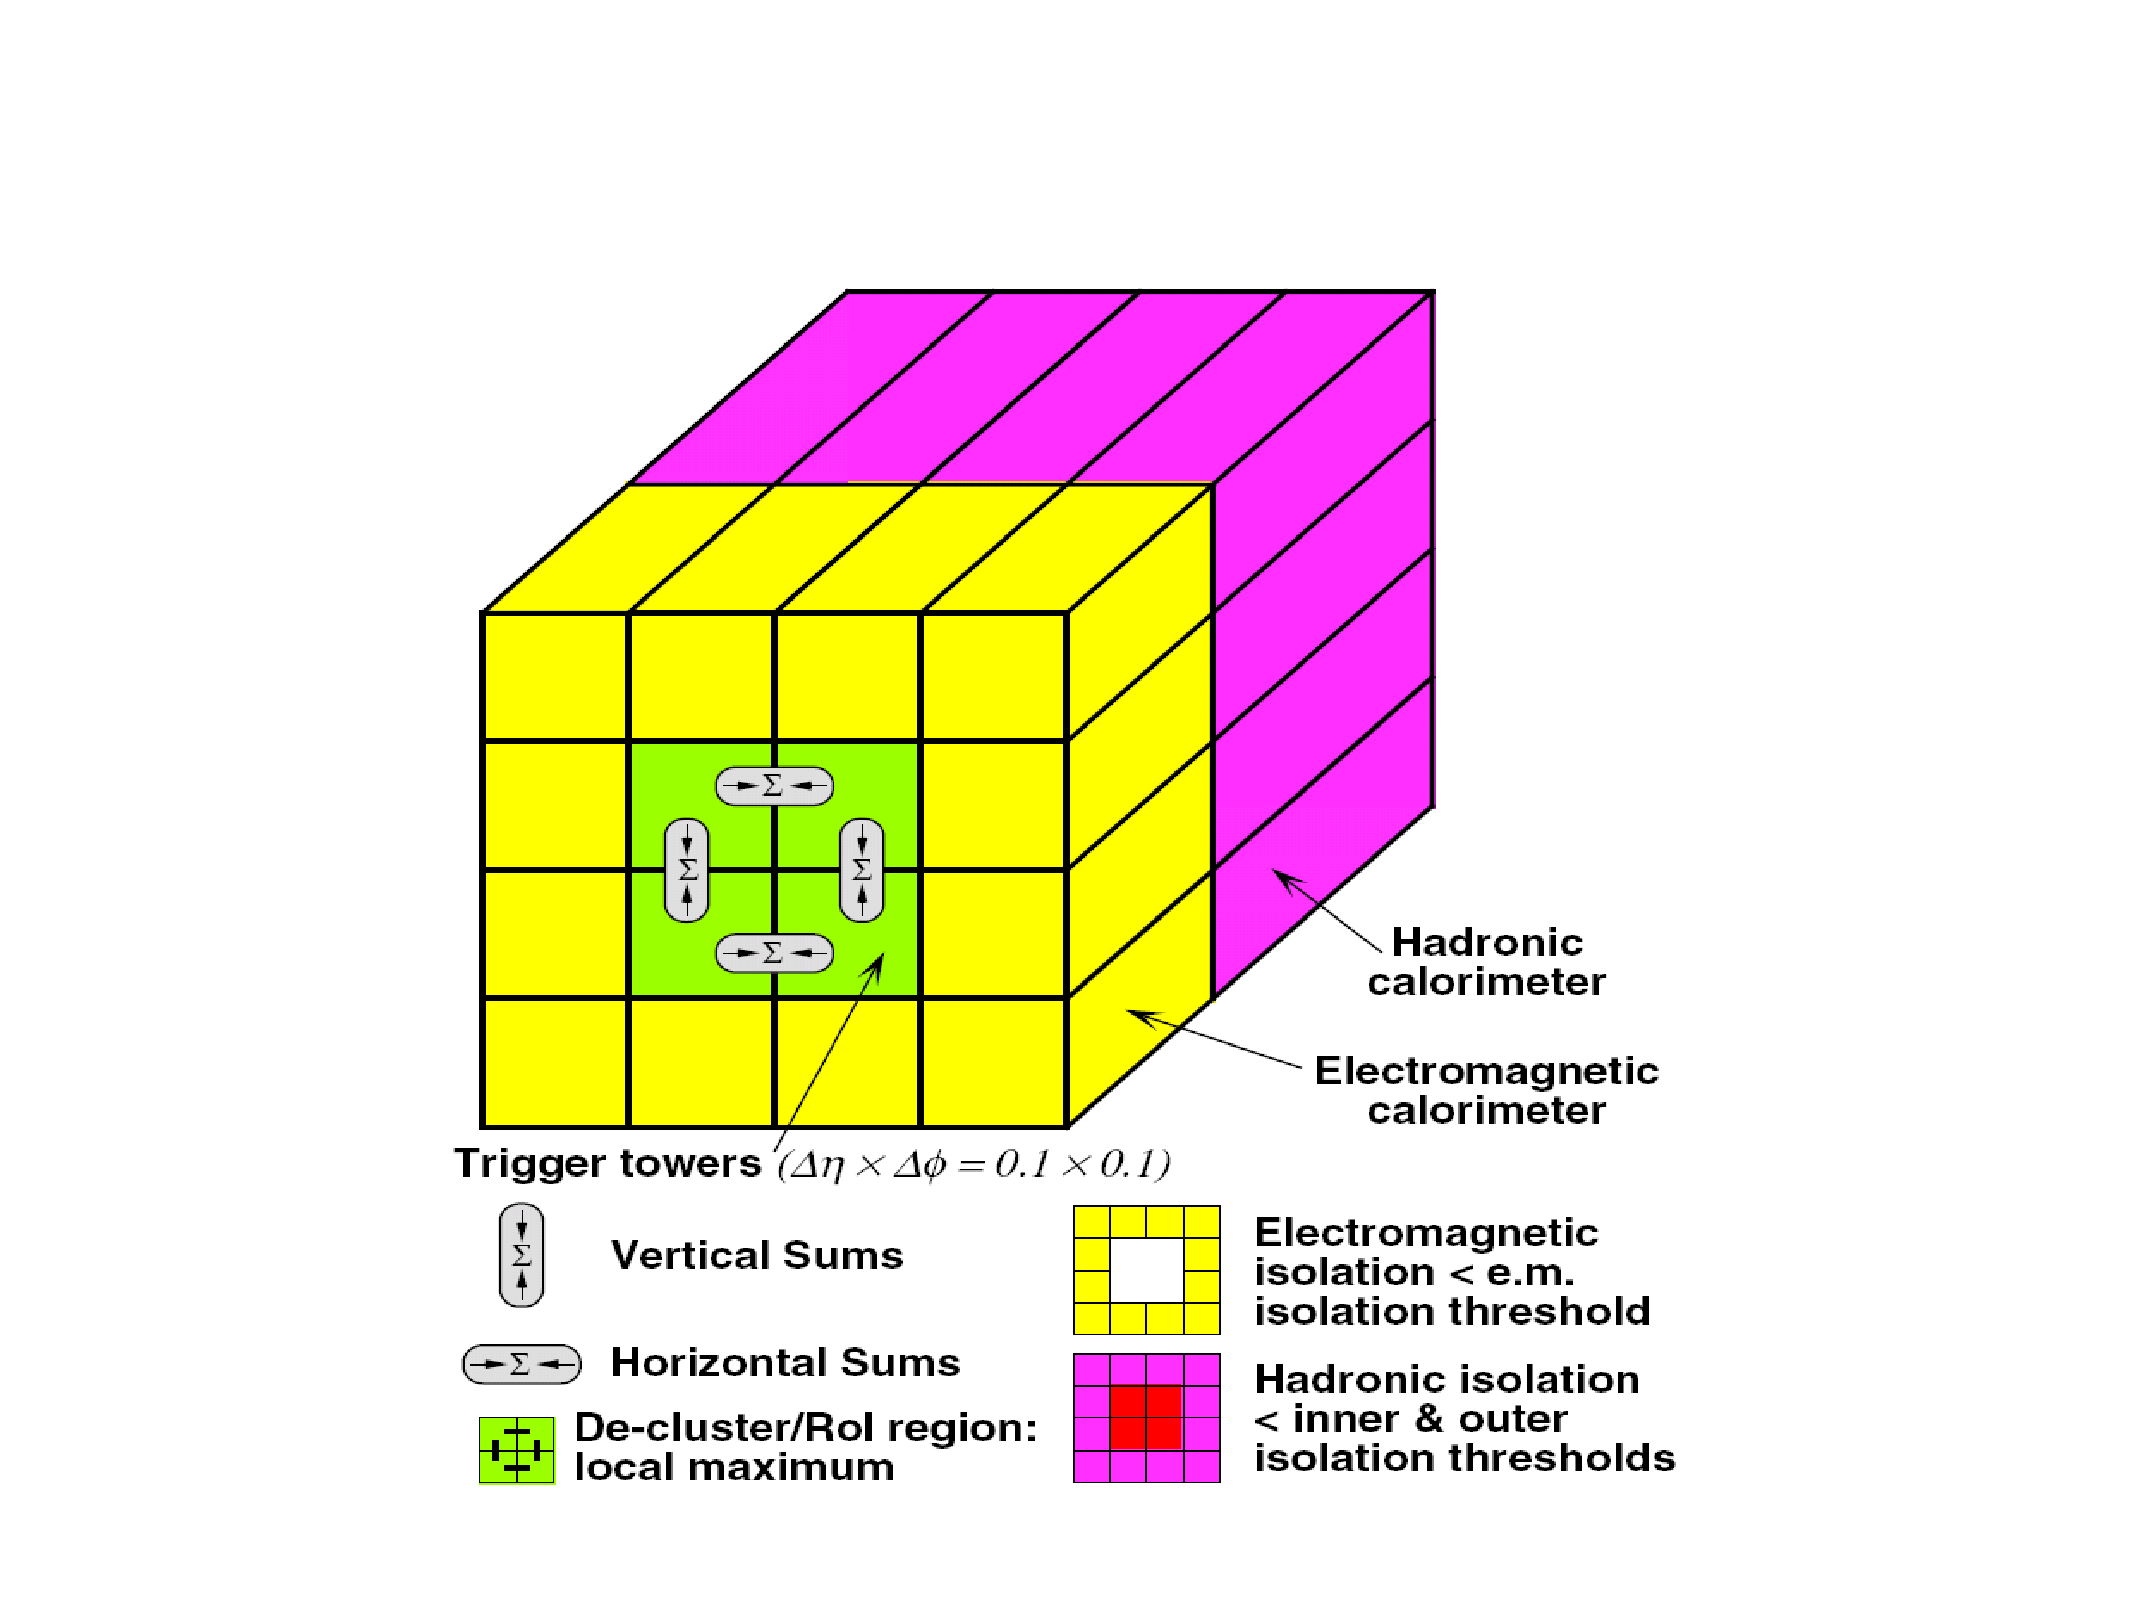
\includegraphics[width=0.80\textwidth]{figures/trigger/cartoonL1}
  \caption{Variables.}
  \label{fig:prospects-trigger-cartoonL1}
\end{figure}

\begin{figure}[tp]
  \centering
  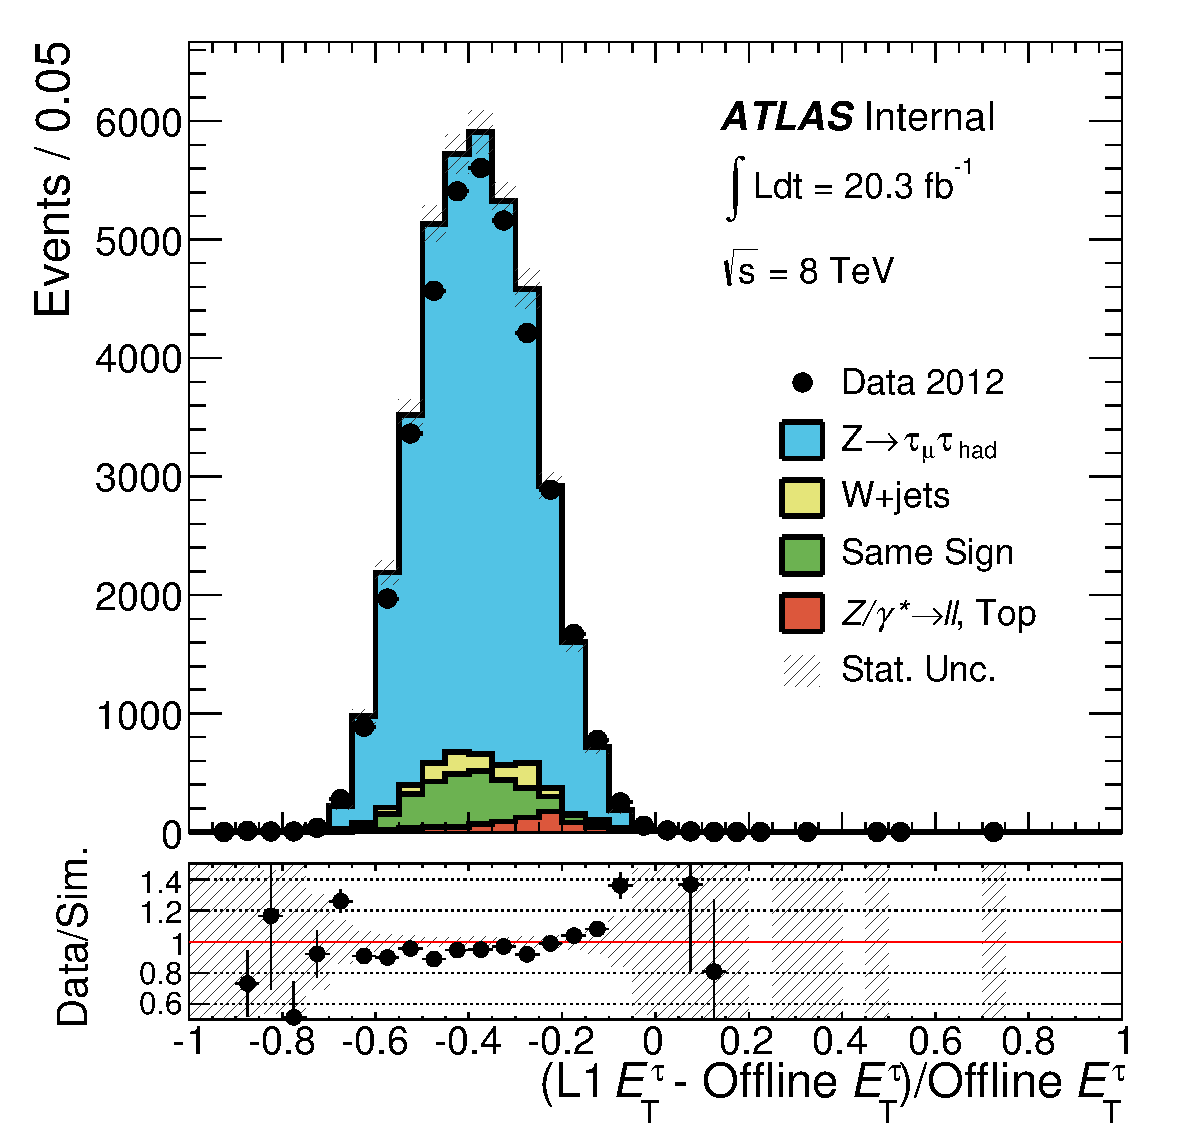
\includegraphics[width=0.48\textwidth]{figures/PERF-2013-06_tmp/tau_trig_2012_resL1_pt}
  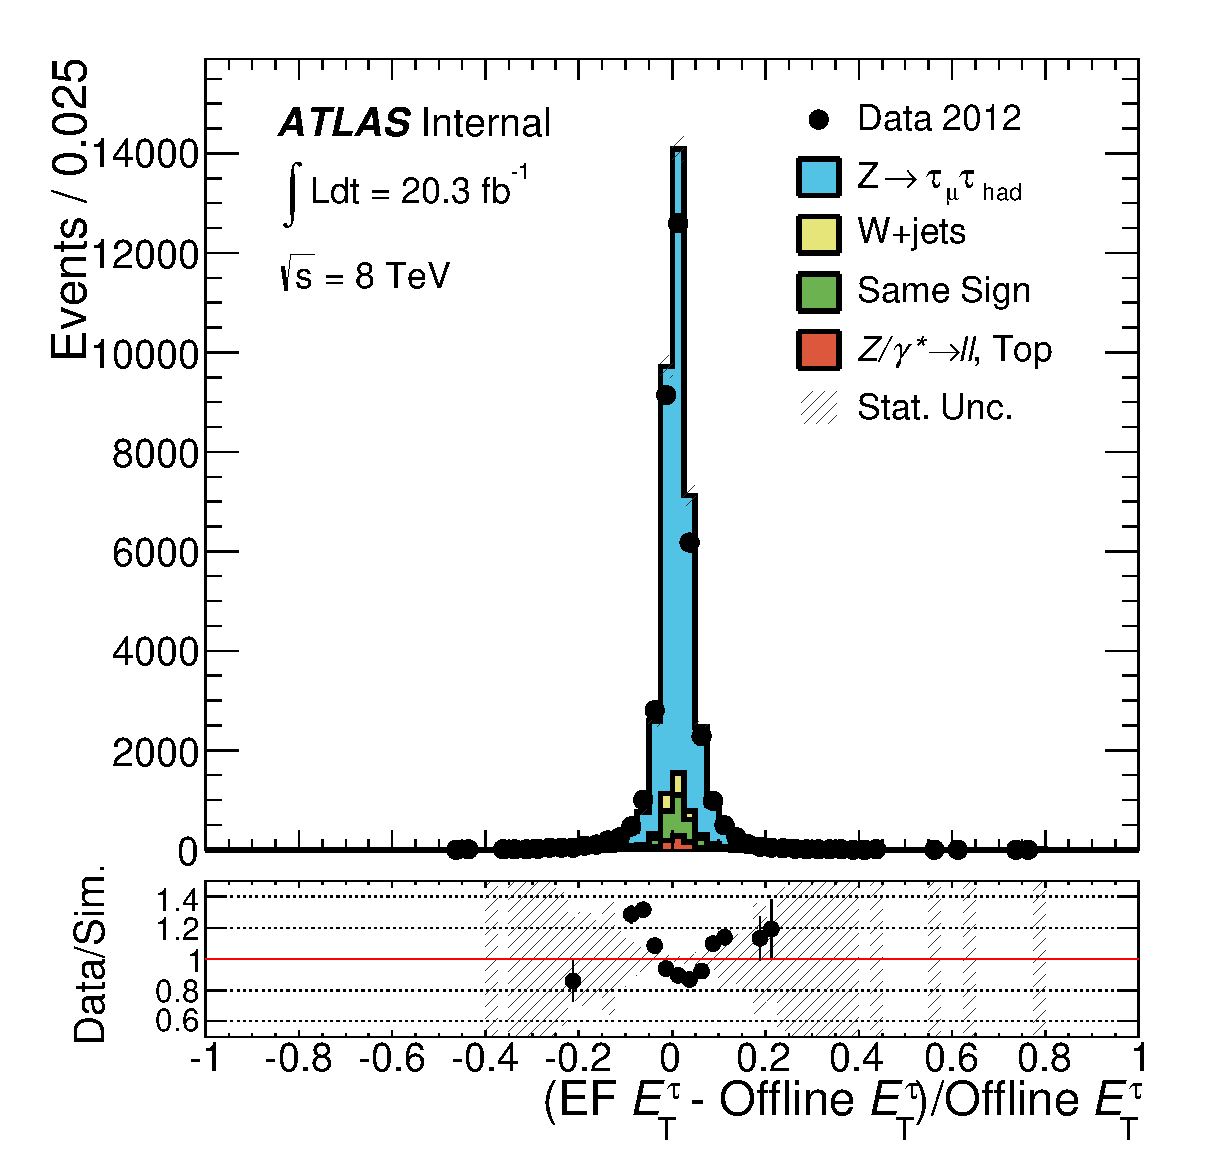
\includegraphics[width=0.48\textwidth]{figures/PERF-2013-06_tmp/tau_trig_2012_resEF_pt}
  \caption{Variables.}
  \label{fig:prospects-trigger-resolution}
\end{figure}

\begin{figure}[tp]
  \centering
  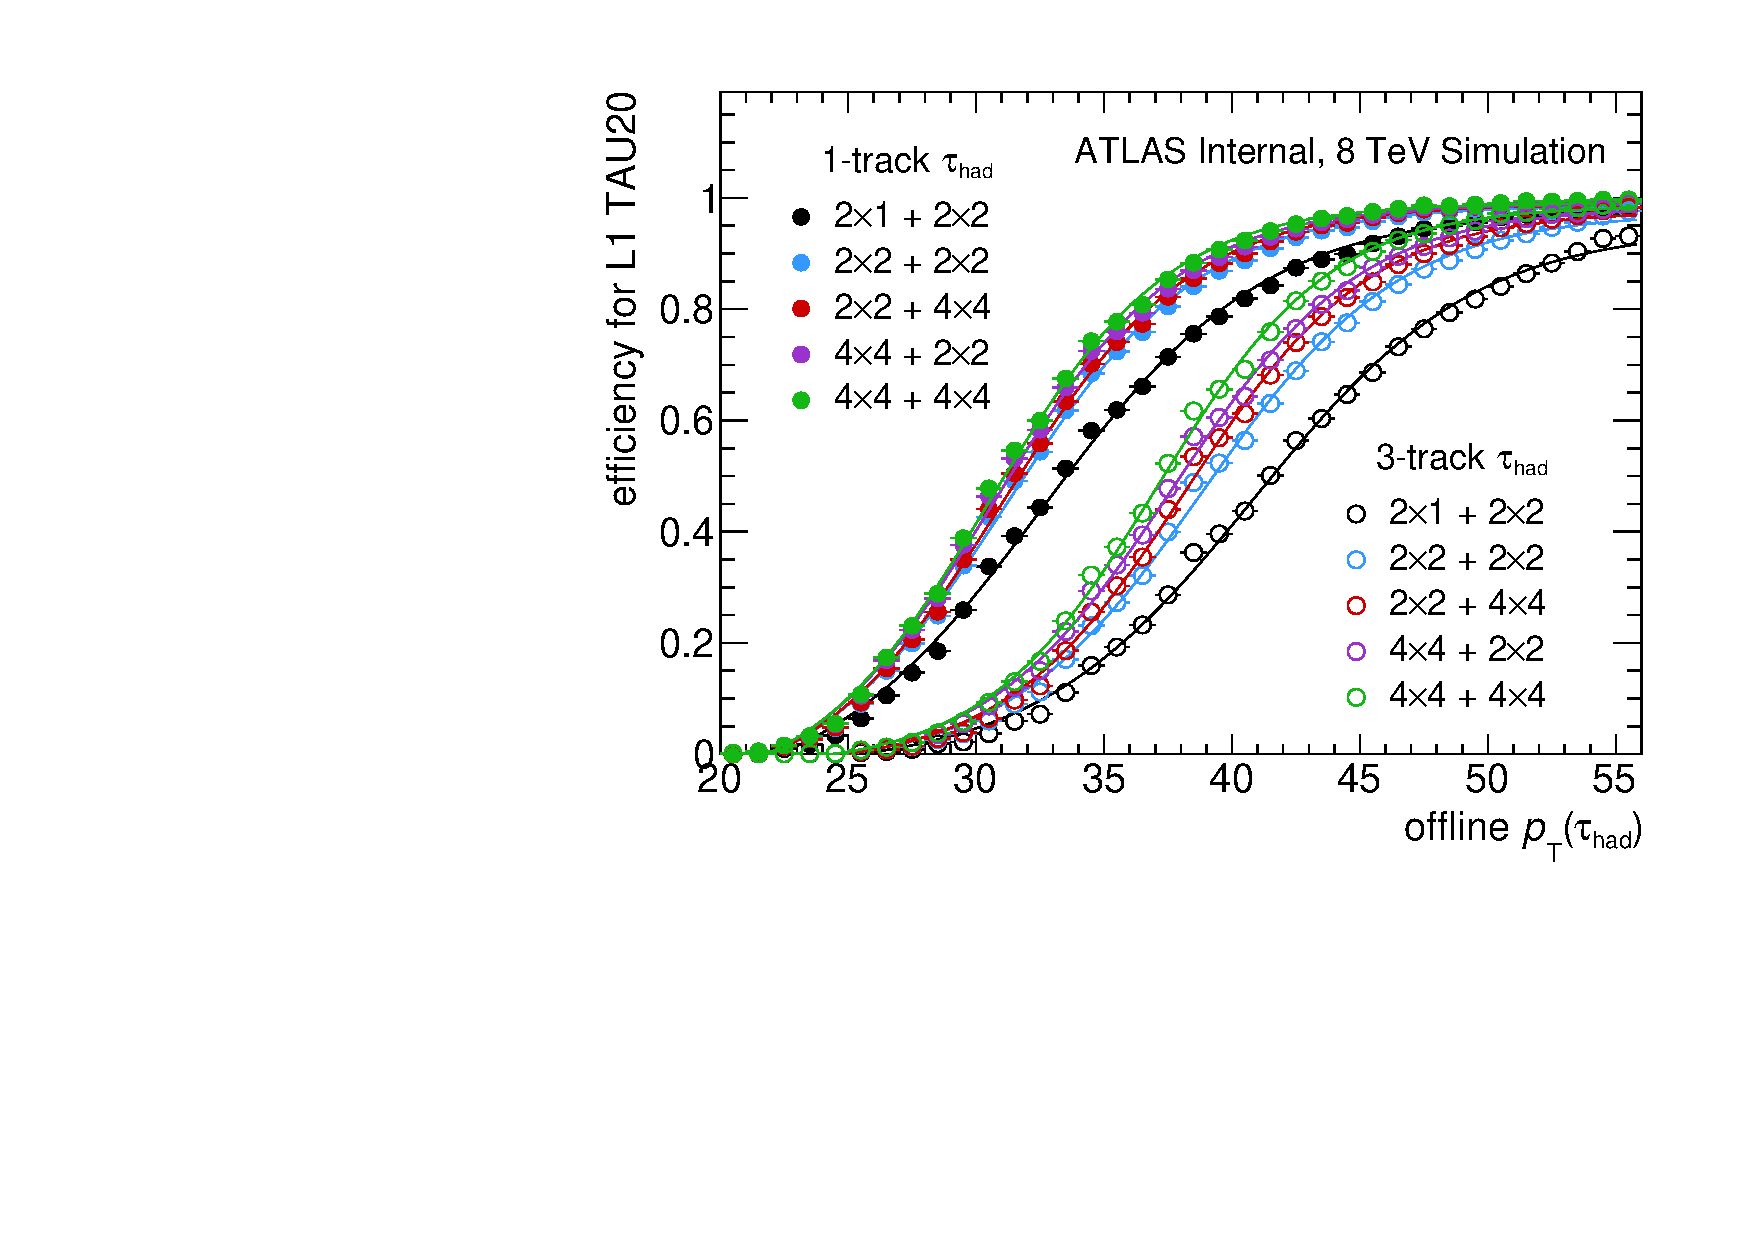
\includegraphics[width=0.48\textwidth]{figures/trigger/turnon_L1TAU20_1p3p}
  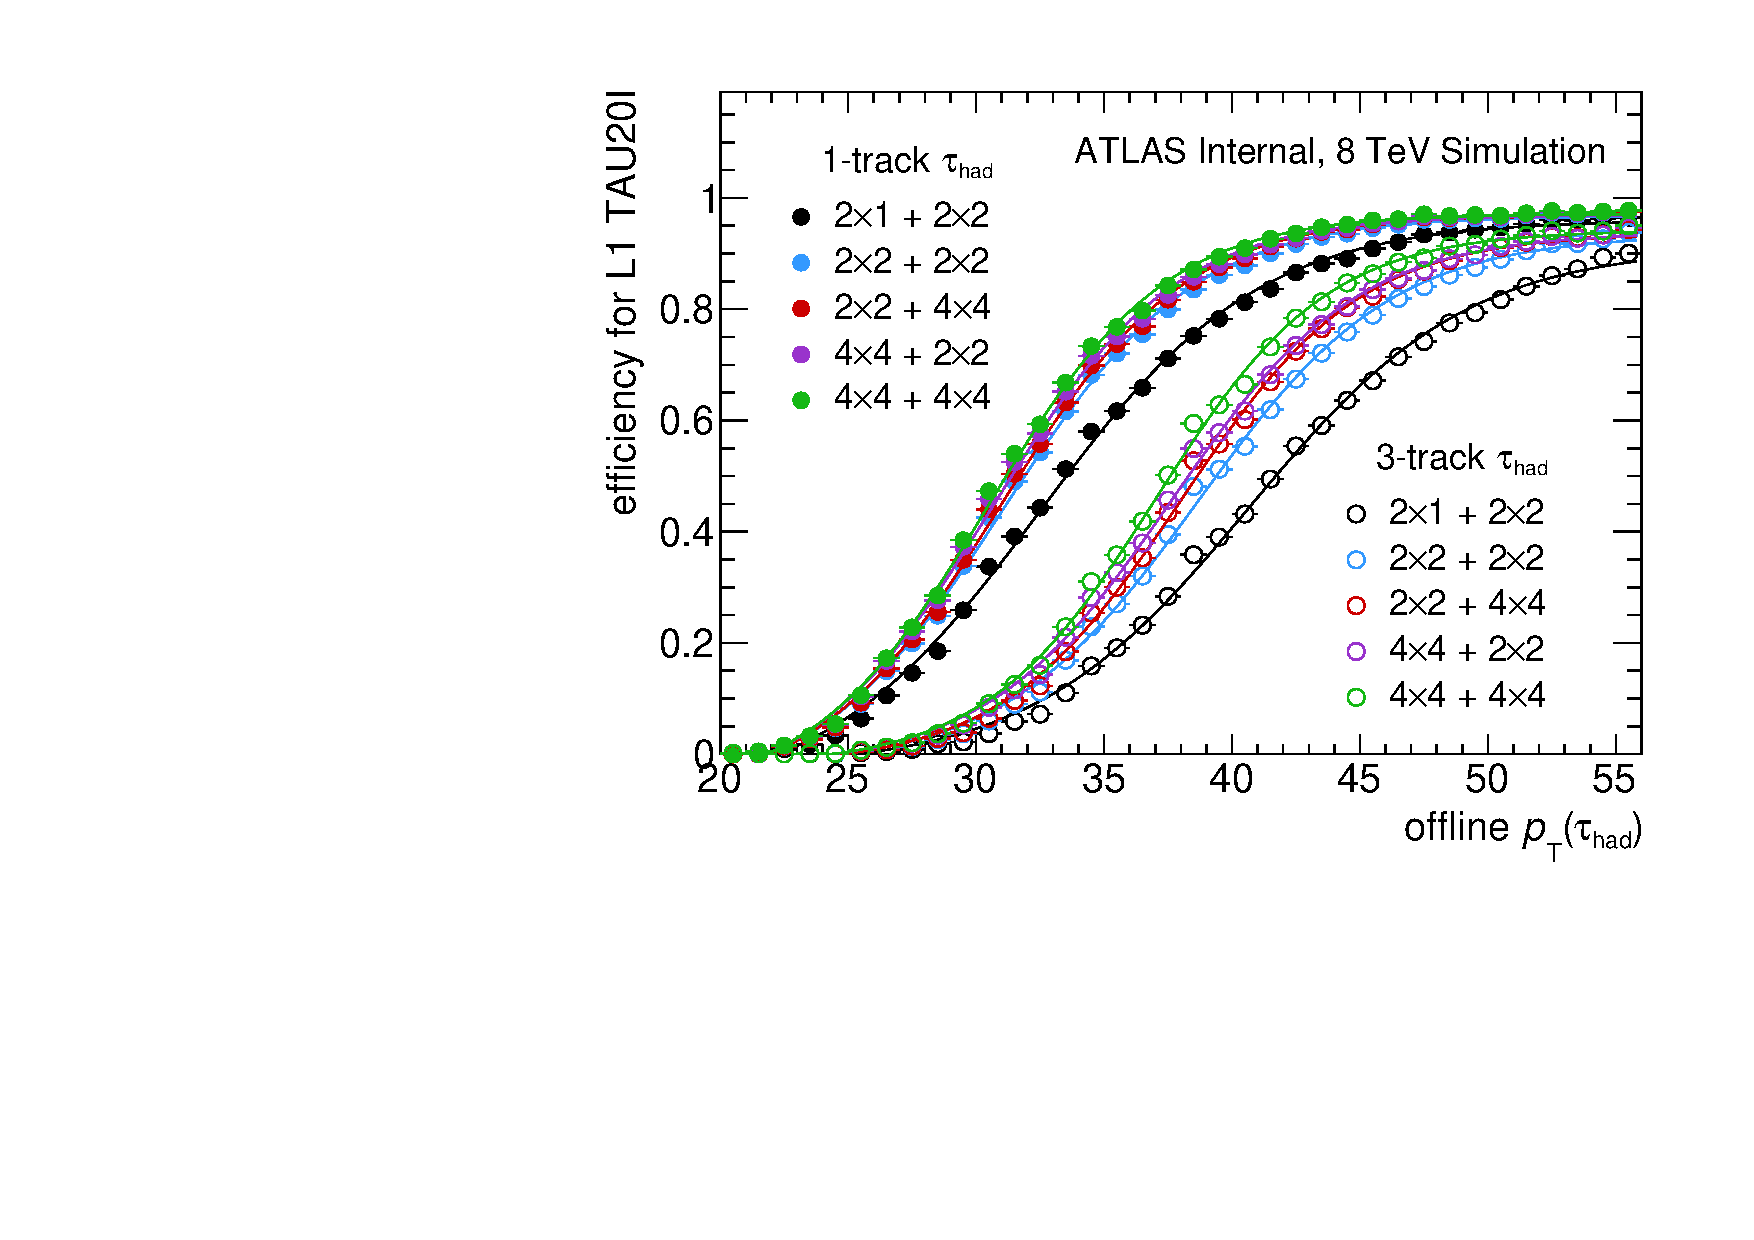
\includegraphics[width=0.48\textwidth]{figures/trigger/turnon_L1TAU20I_1p3p}
  \caption{Variables.}
  \label{fig:prospects-trigger-towersize}
\end{figure}

\begin{figure}[tp]
  \centering
  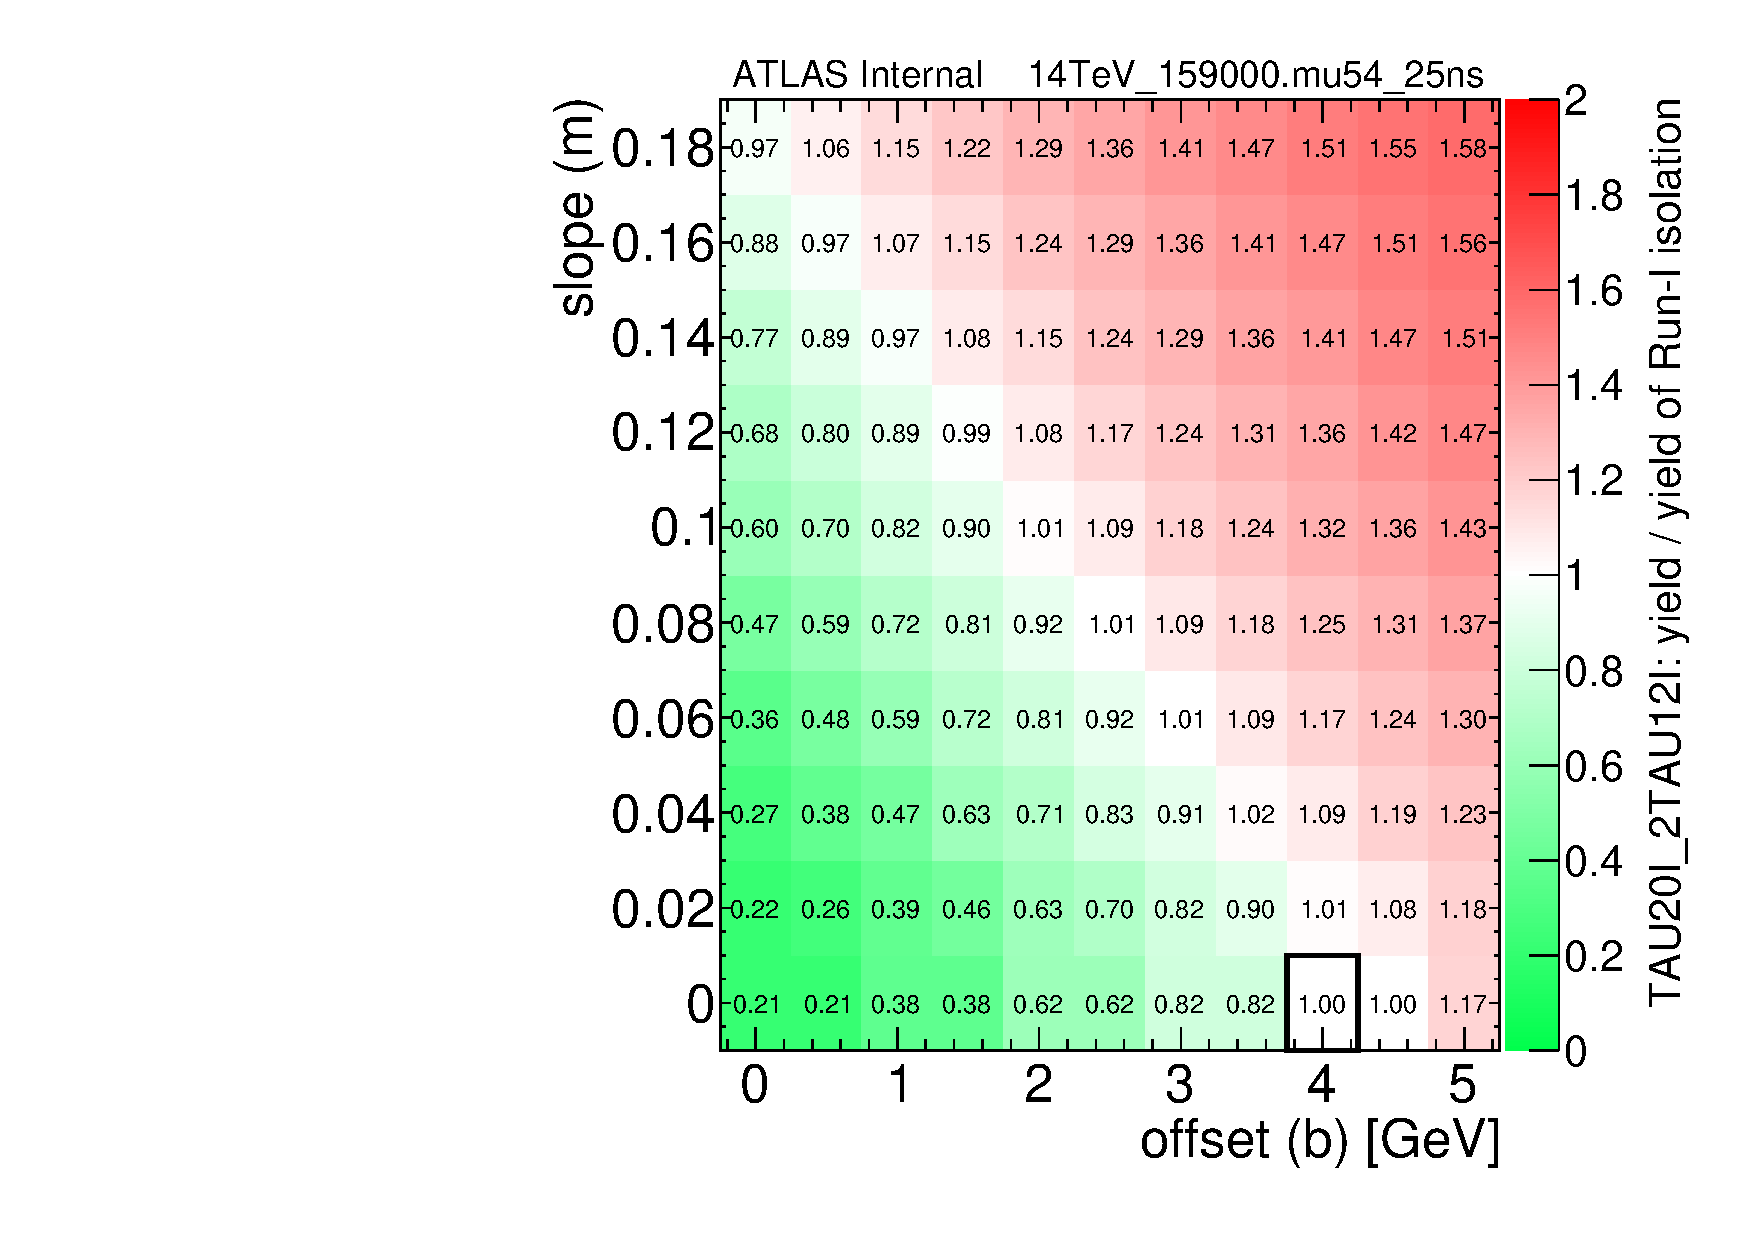
\includegraphics[width=0.48\textwidth]{figures/trigger/iso_background_noTAU60}
  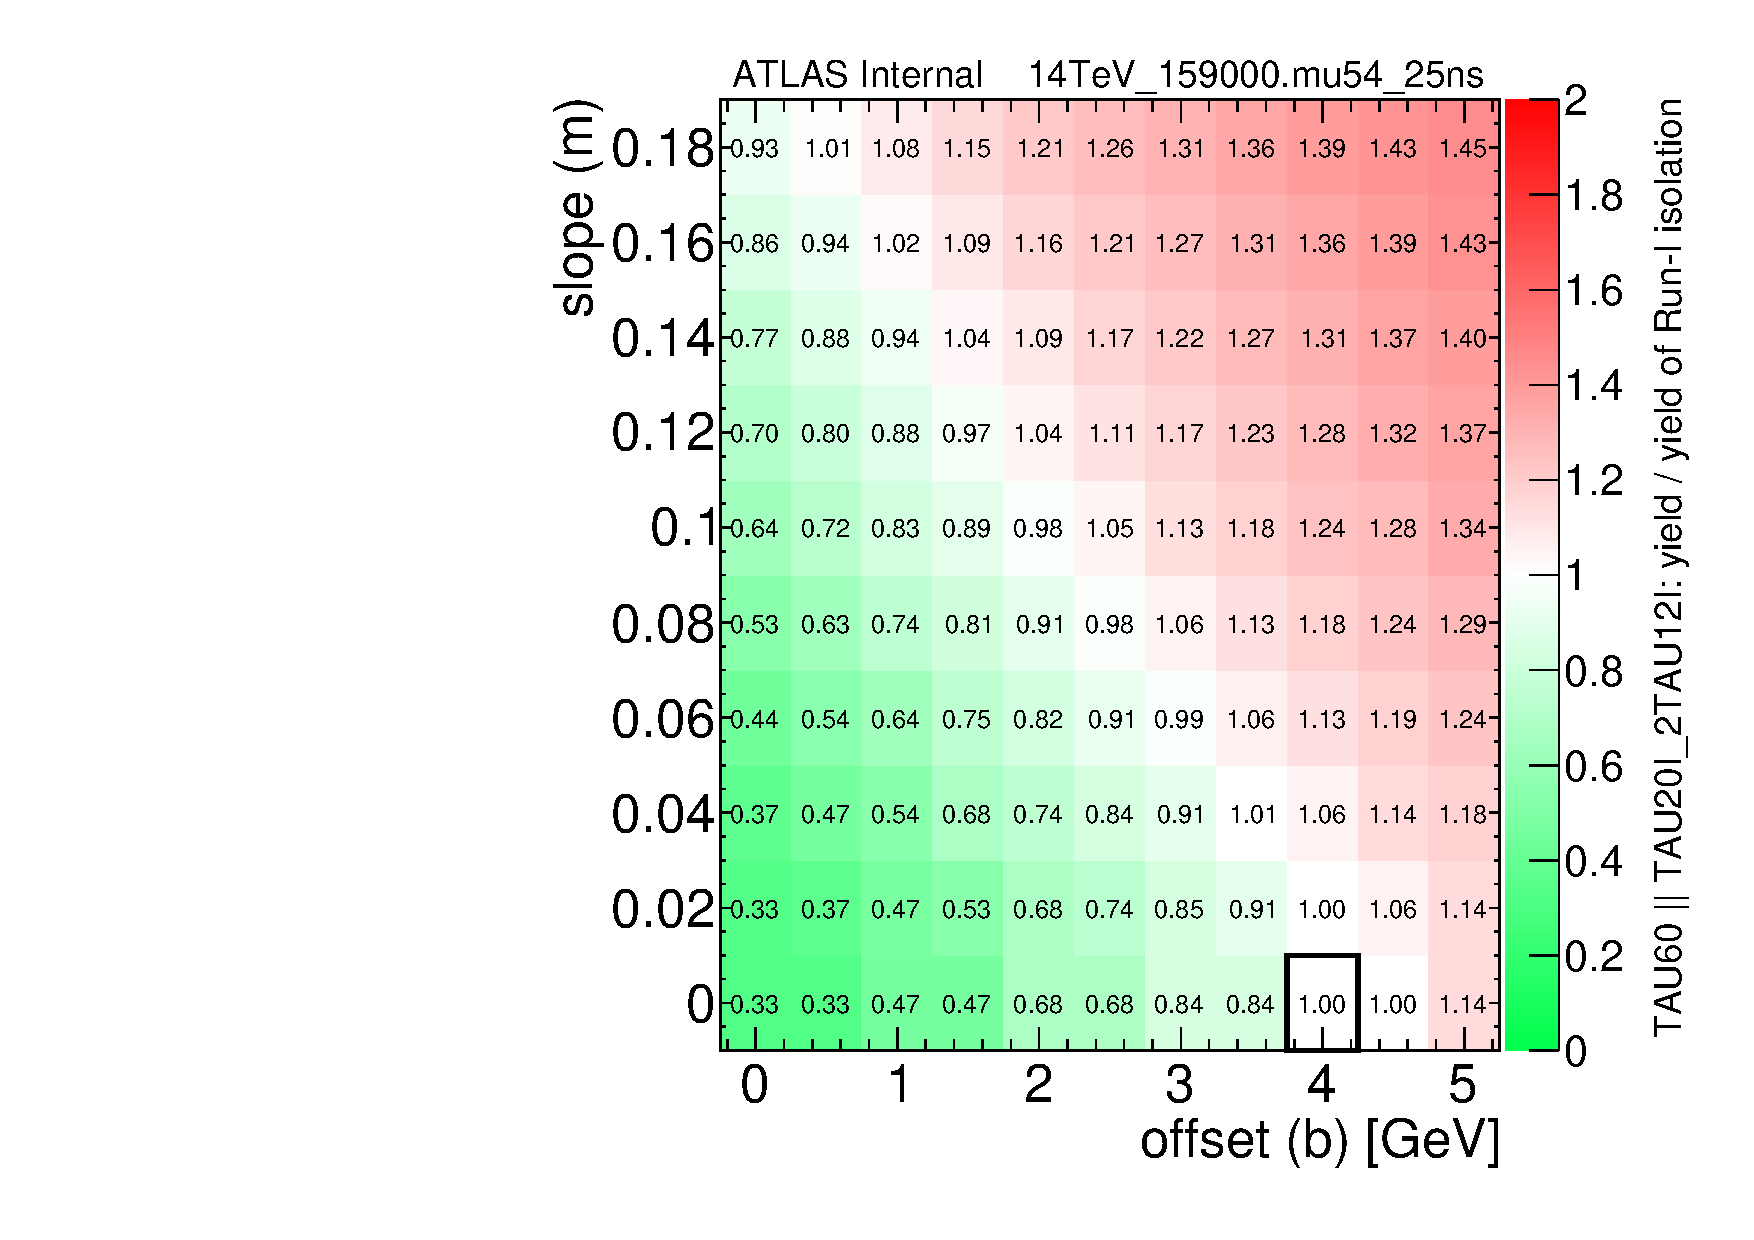
\includegraphics[width=0.48\textwidth]{figures/trigger/iso_background_yesTAU60}
  \caption{Variables.}
  \label{fig:prospects-trigger-isolation-rate}
\end{figure}

\begin{figure}[tp]
  \centering
  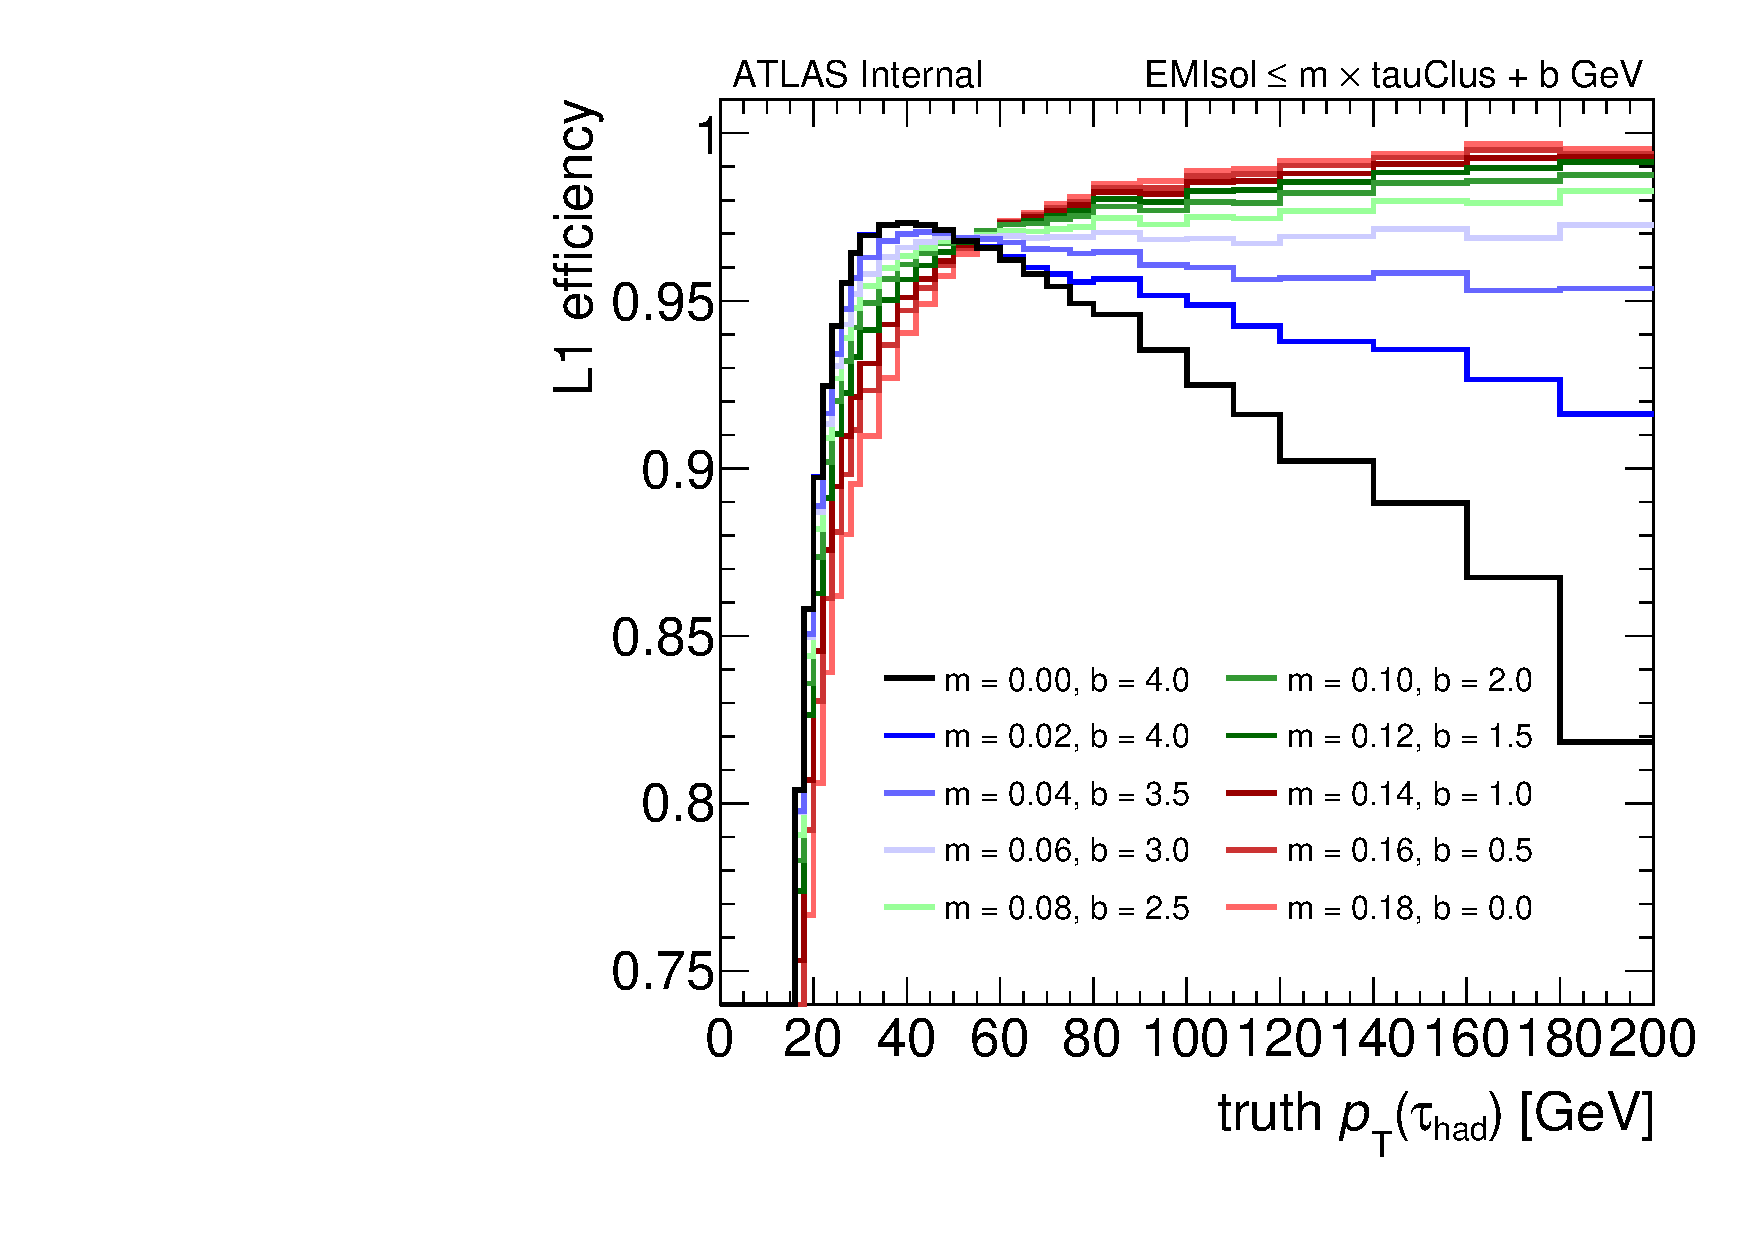
\includegraphics[width=0.48\textwidth]{figures/trigger/iso_turnonL1_noTAU60}
  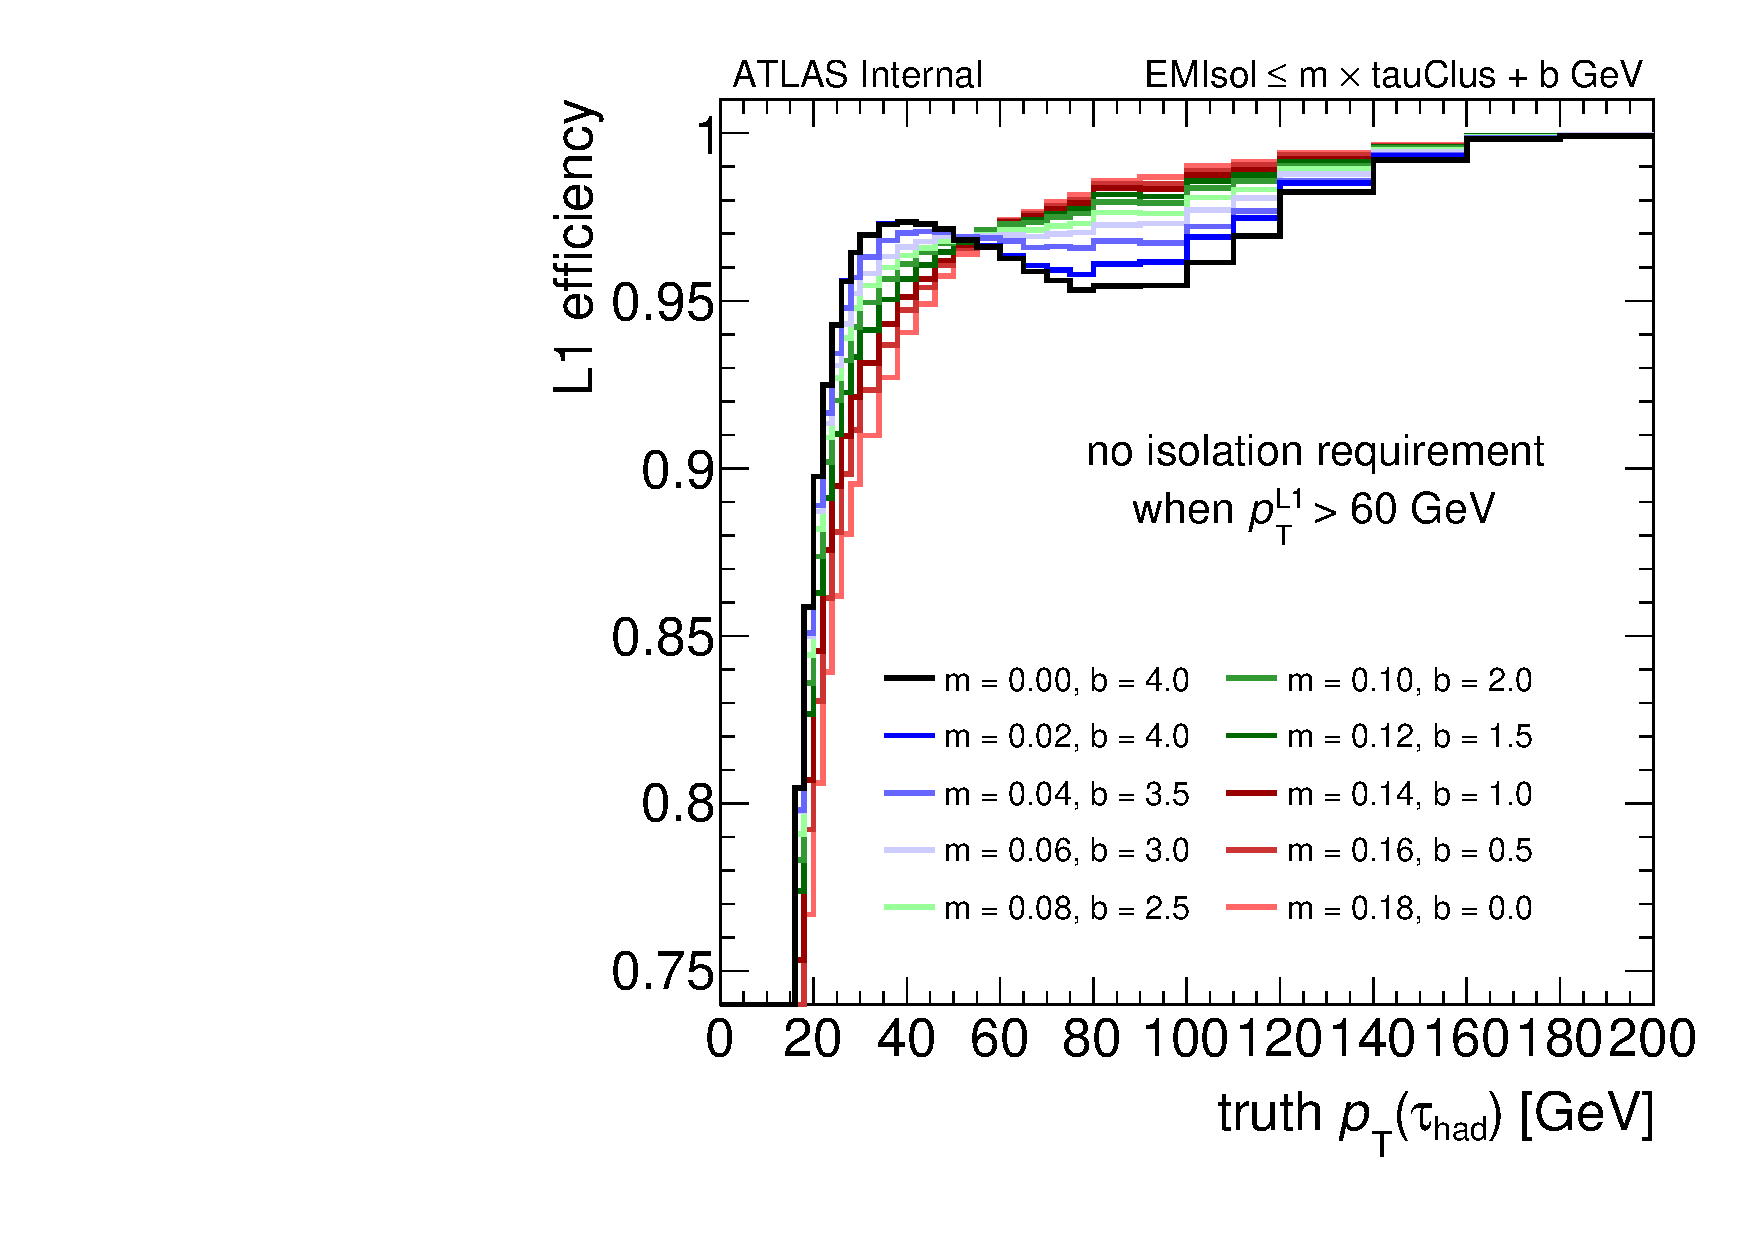
\includegraphics[width=0.48\textwidth]{figures/trigger/iso_turnonL1_yesTAU60}
  \caption{Variables.}
  \label{fig:prospects-trigger-isolation-turnon}
\end{figure}

\begin{figure}[tp]
  \centering
  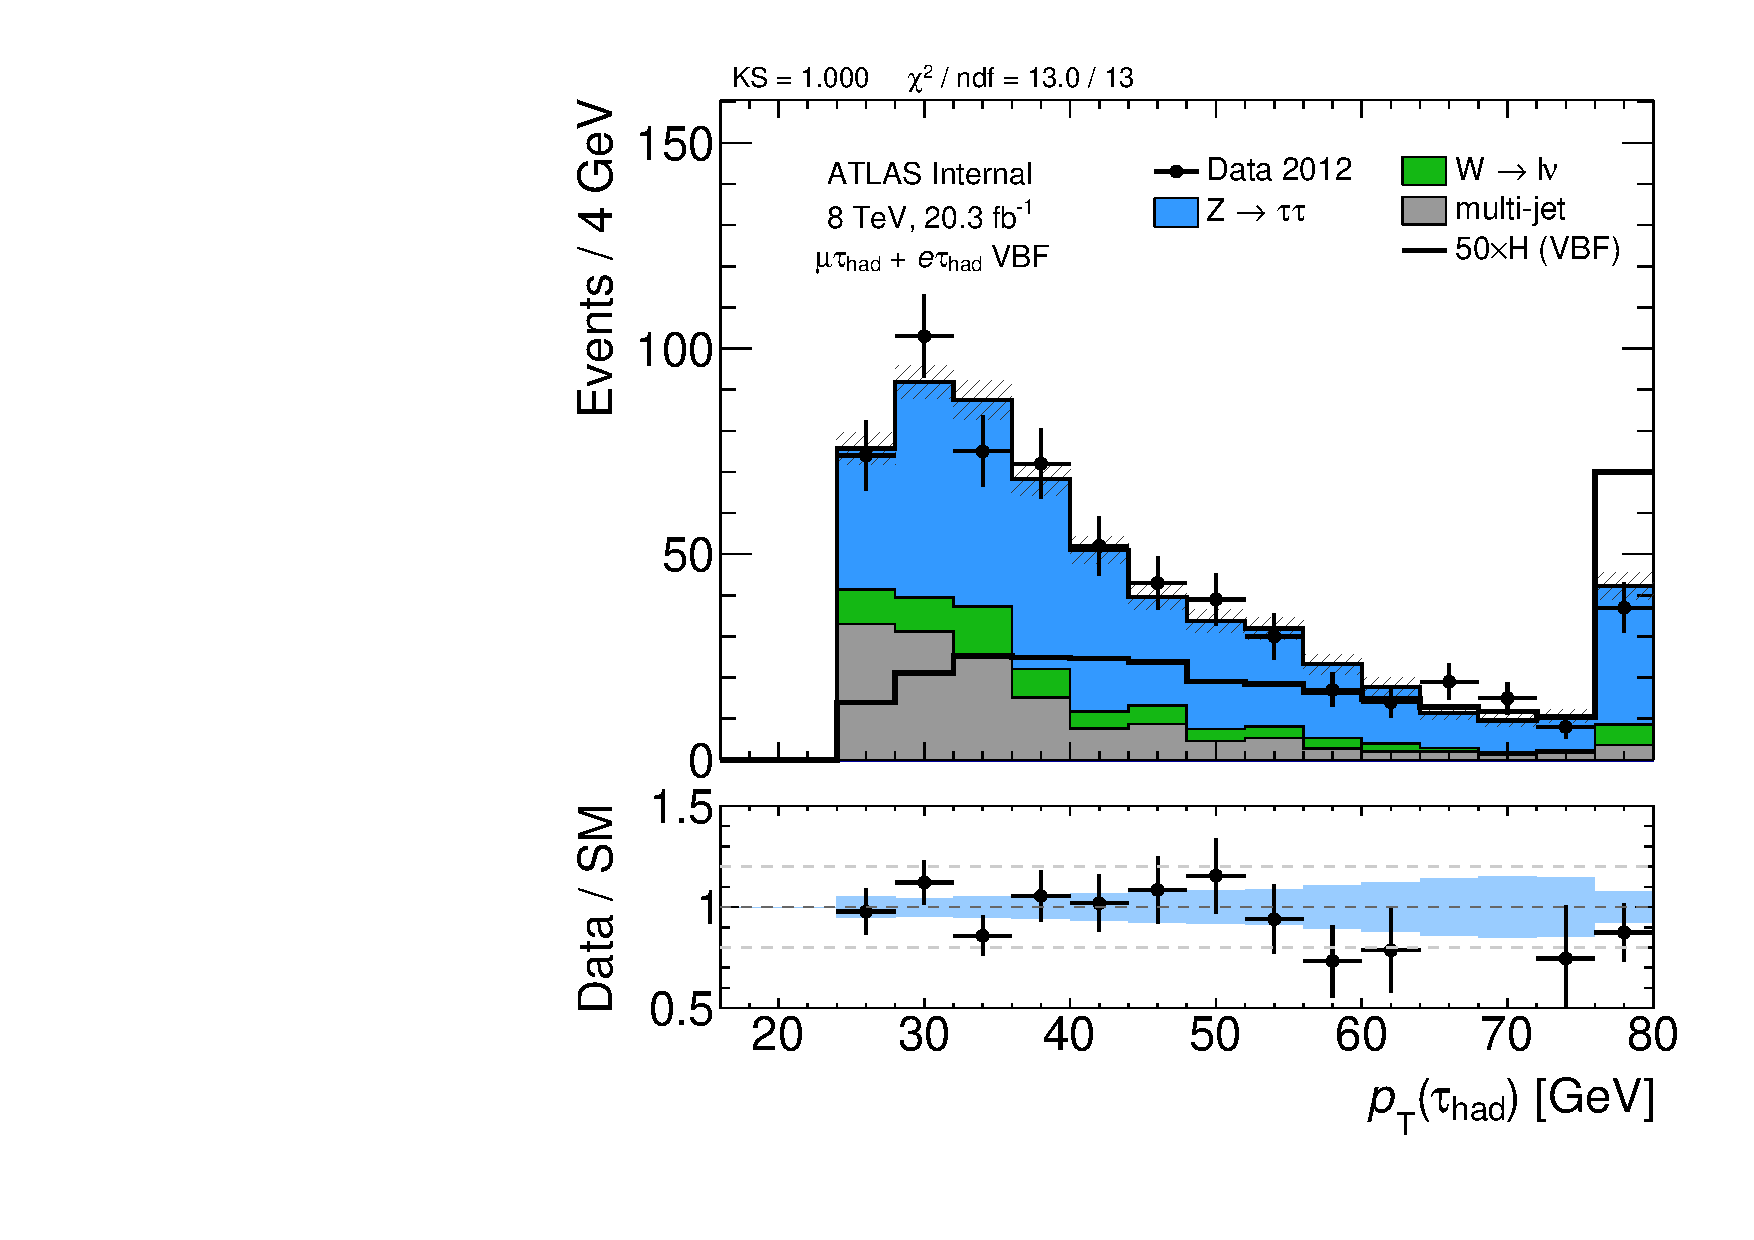
\includegraphics[width=0.32\textwidth]{figures/vbf-LTT/tau-pt}
  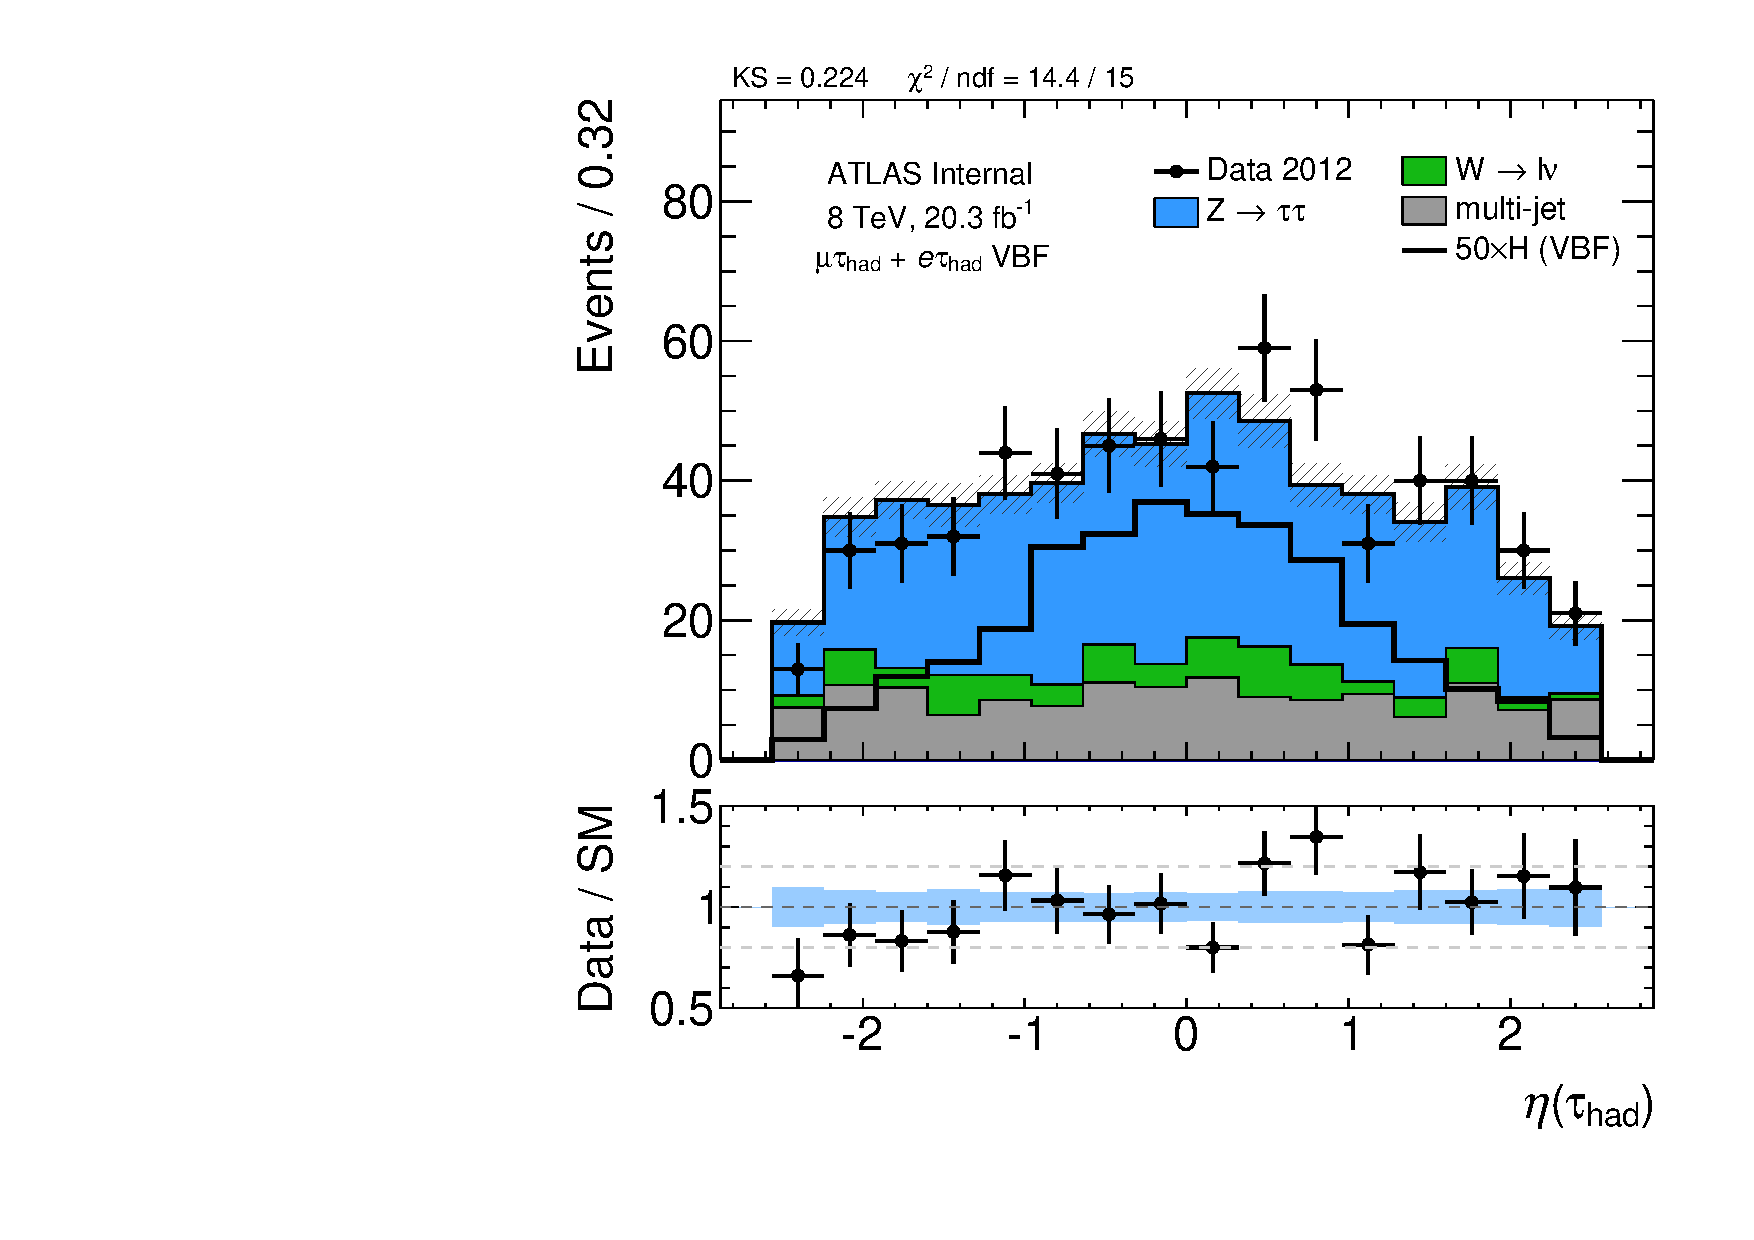
\includegraphics[width=0.32\textwidth]{figures/vbf-LTT/tau-eta}
  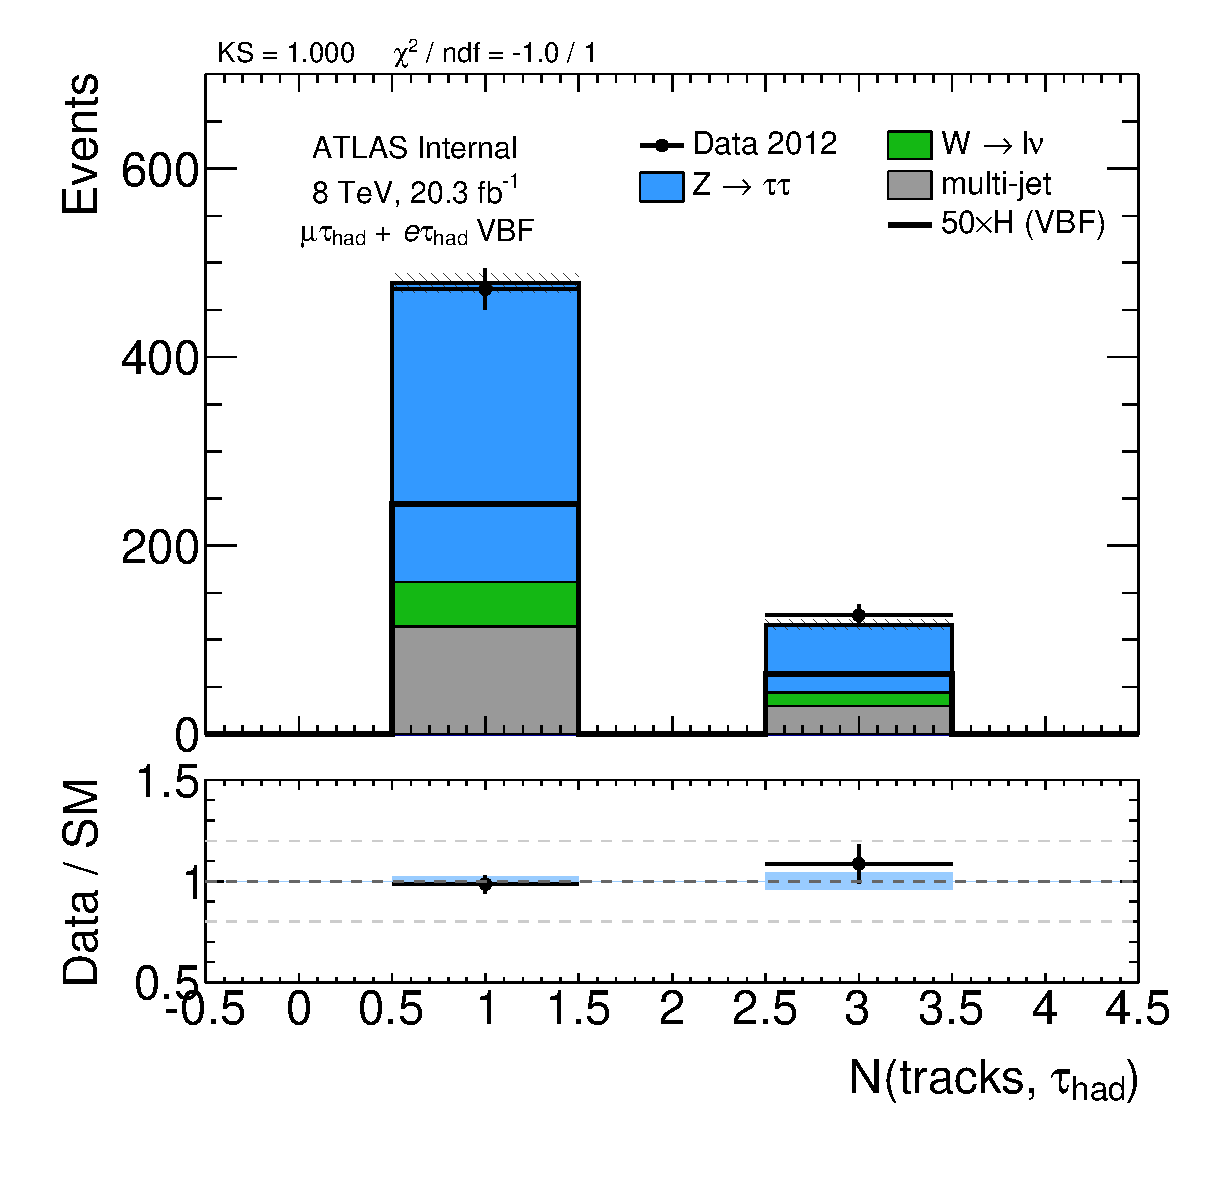
\includegraphics[width=0.32\textwidth]{figures/vbf-LTT/tau-numTrack}
  % --------------
  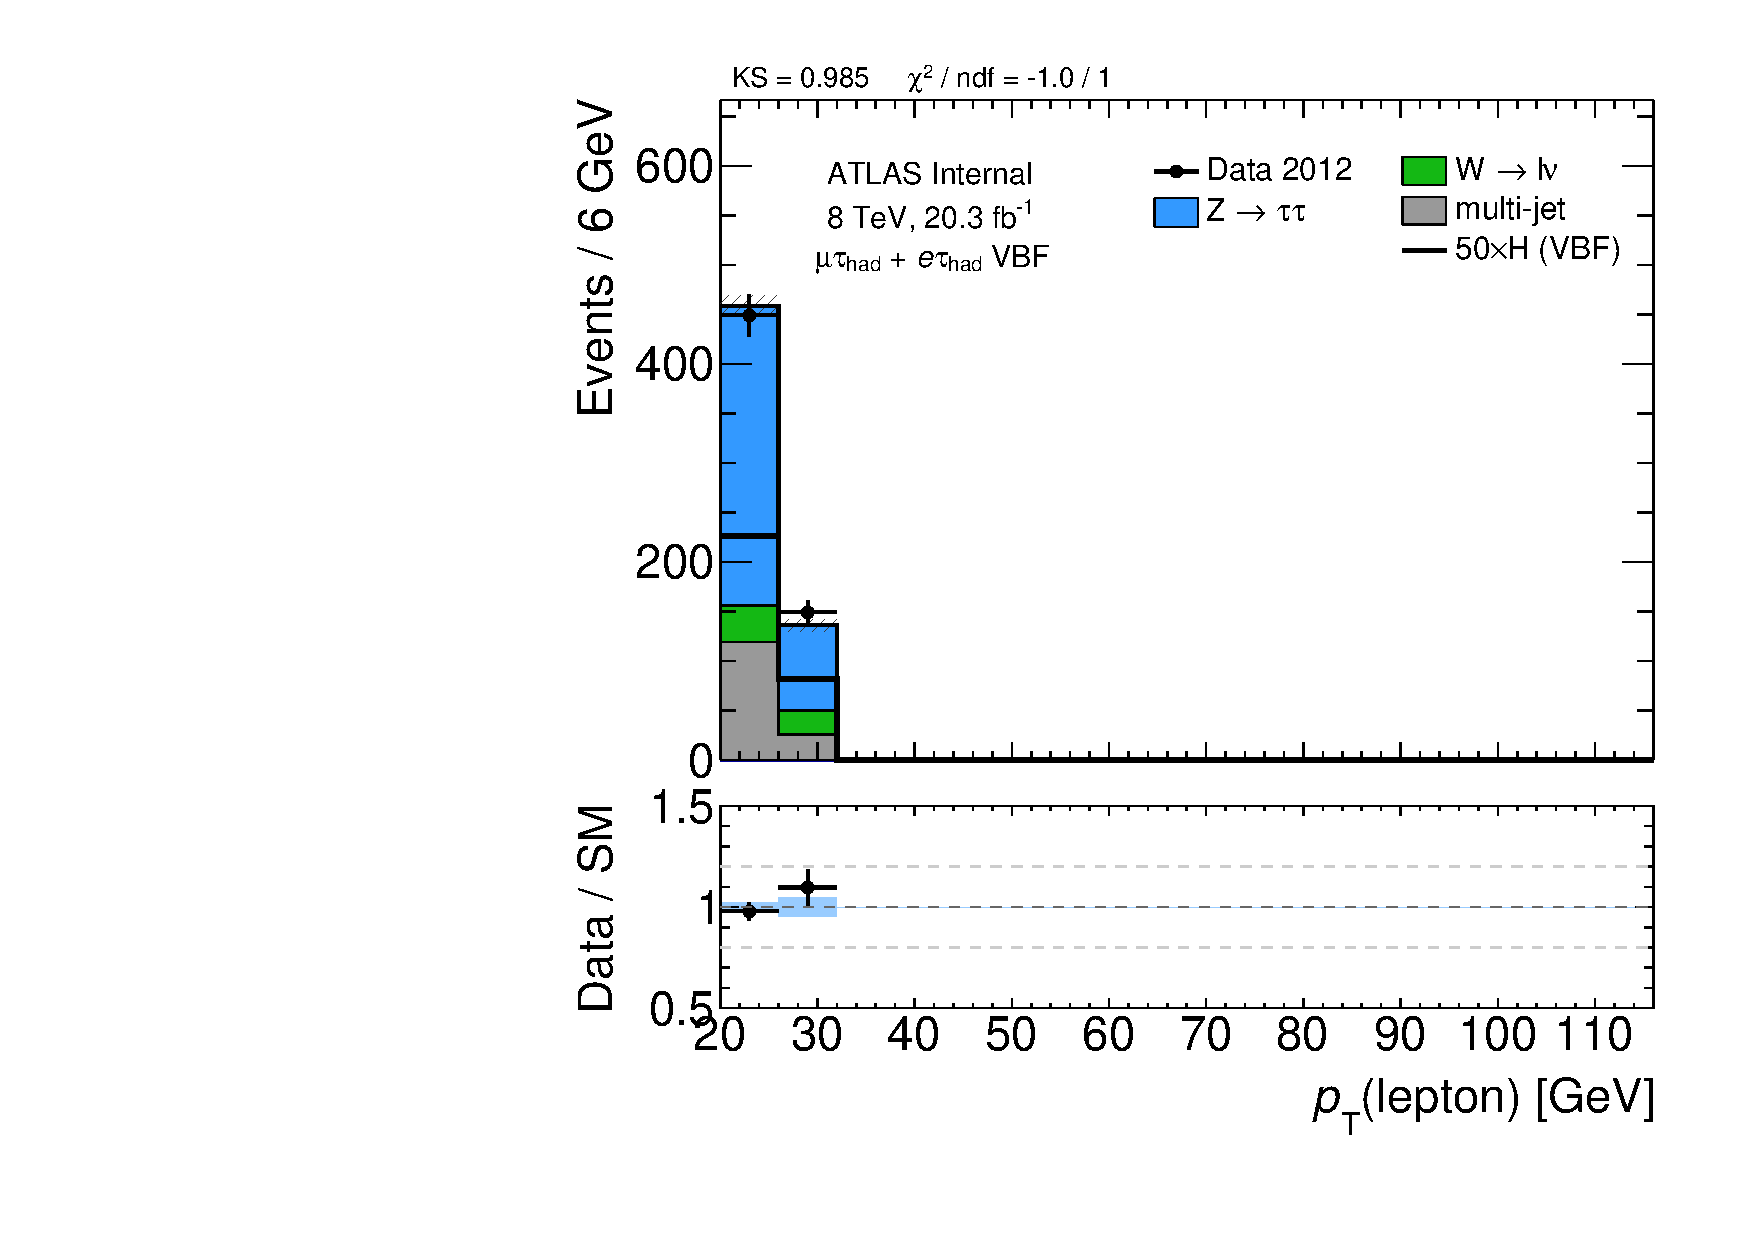
\includegraphics[width=0.32\textwidth]{figures/vbf-LTT/lep-pt-hi}
  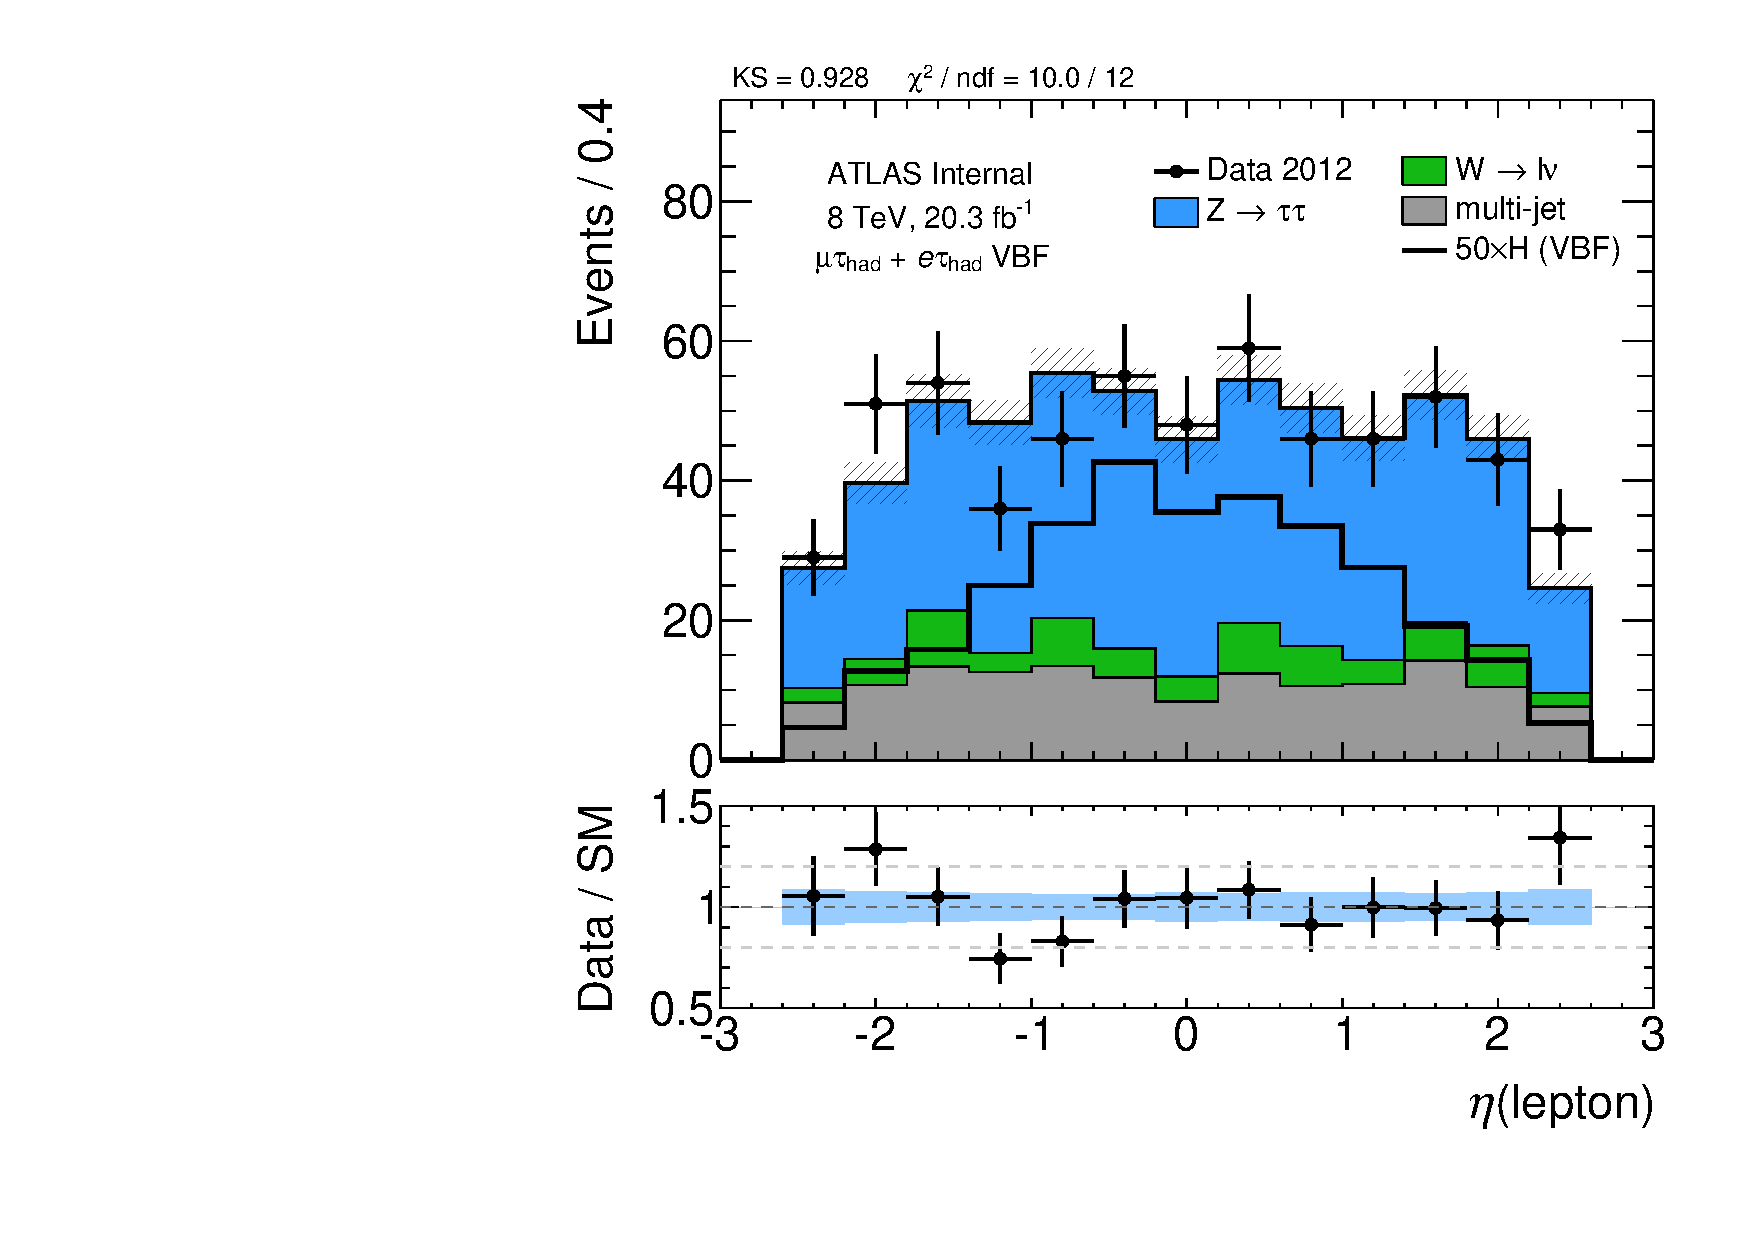
\includegraphics[width=0.32\textwidth]{figures/vbf-LTT/lep-eta}
  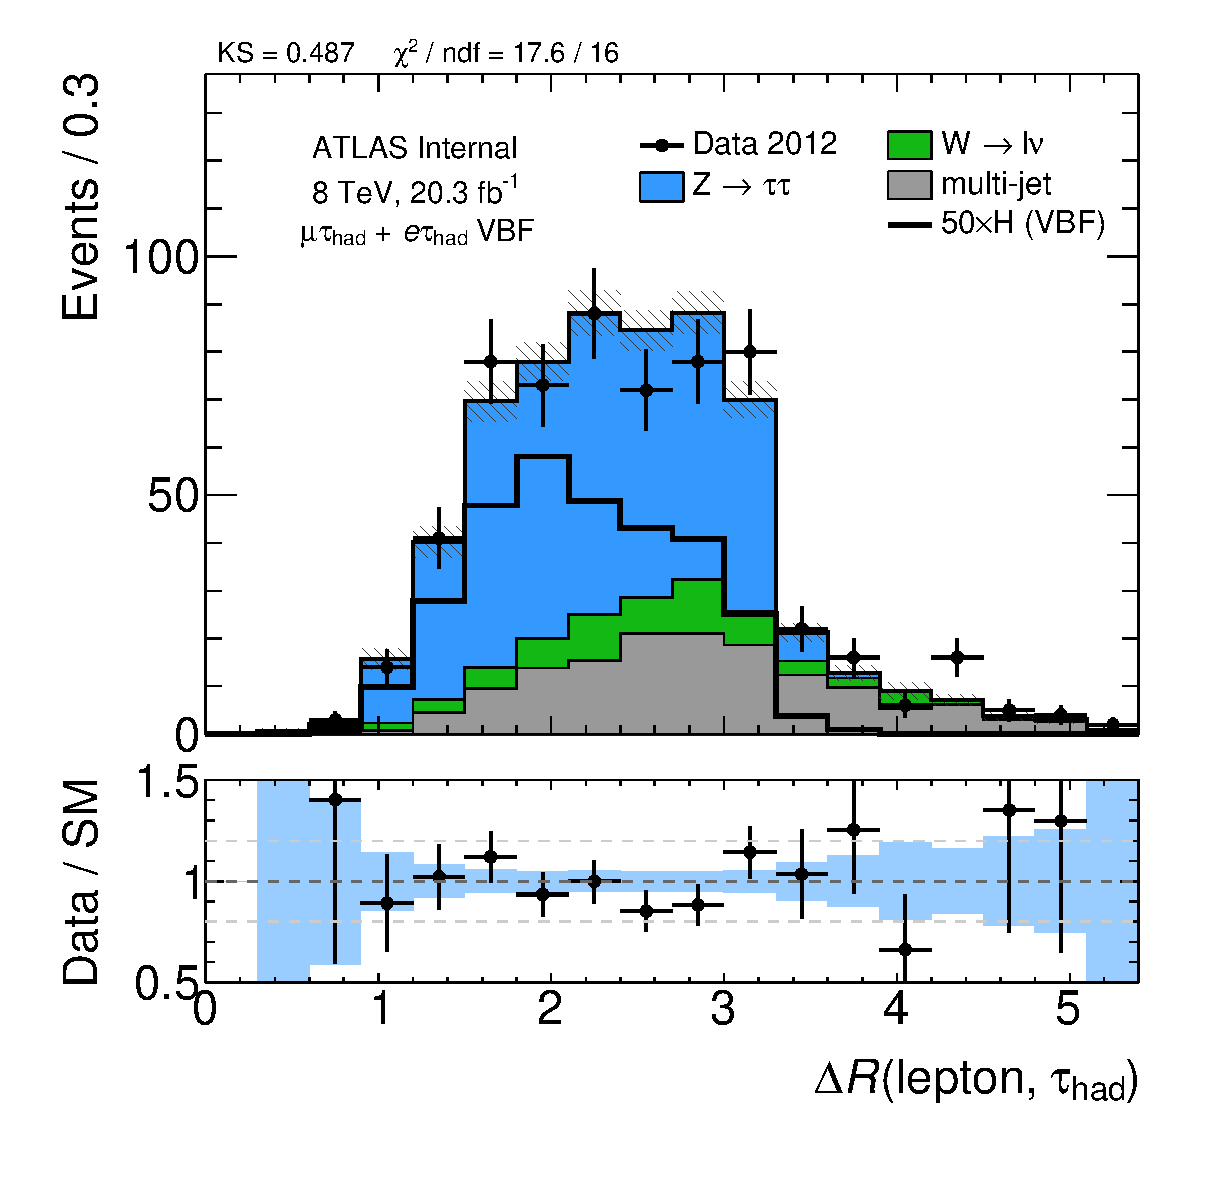
\includegraphics[width=0.32\textwidth]{figures/vbf-LTT/taulep-dR}
  % --------------
  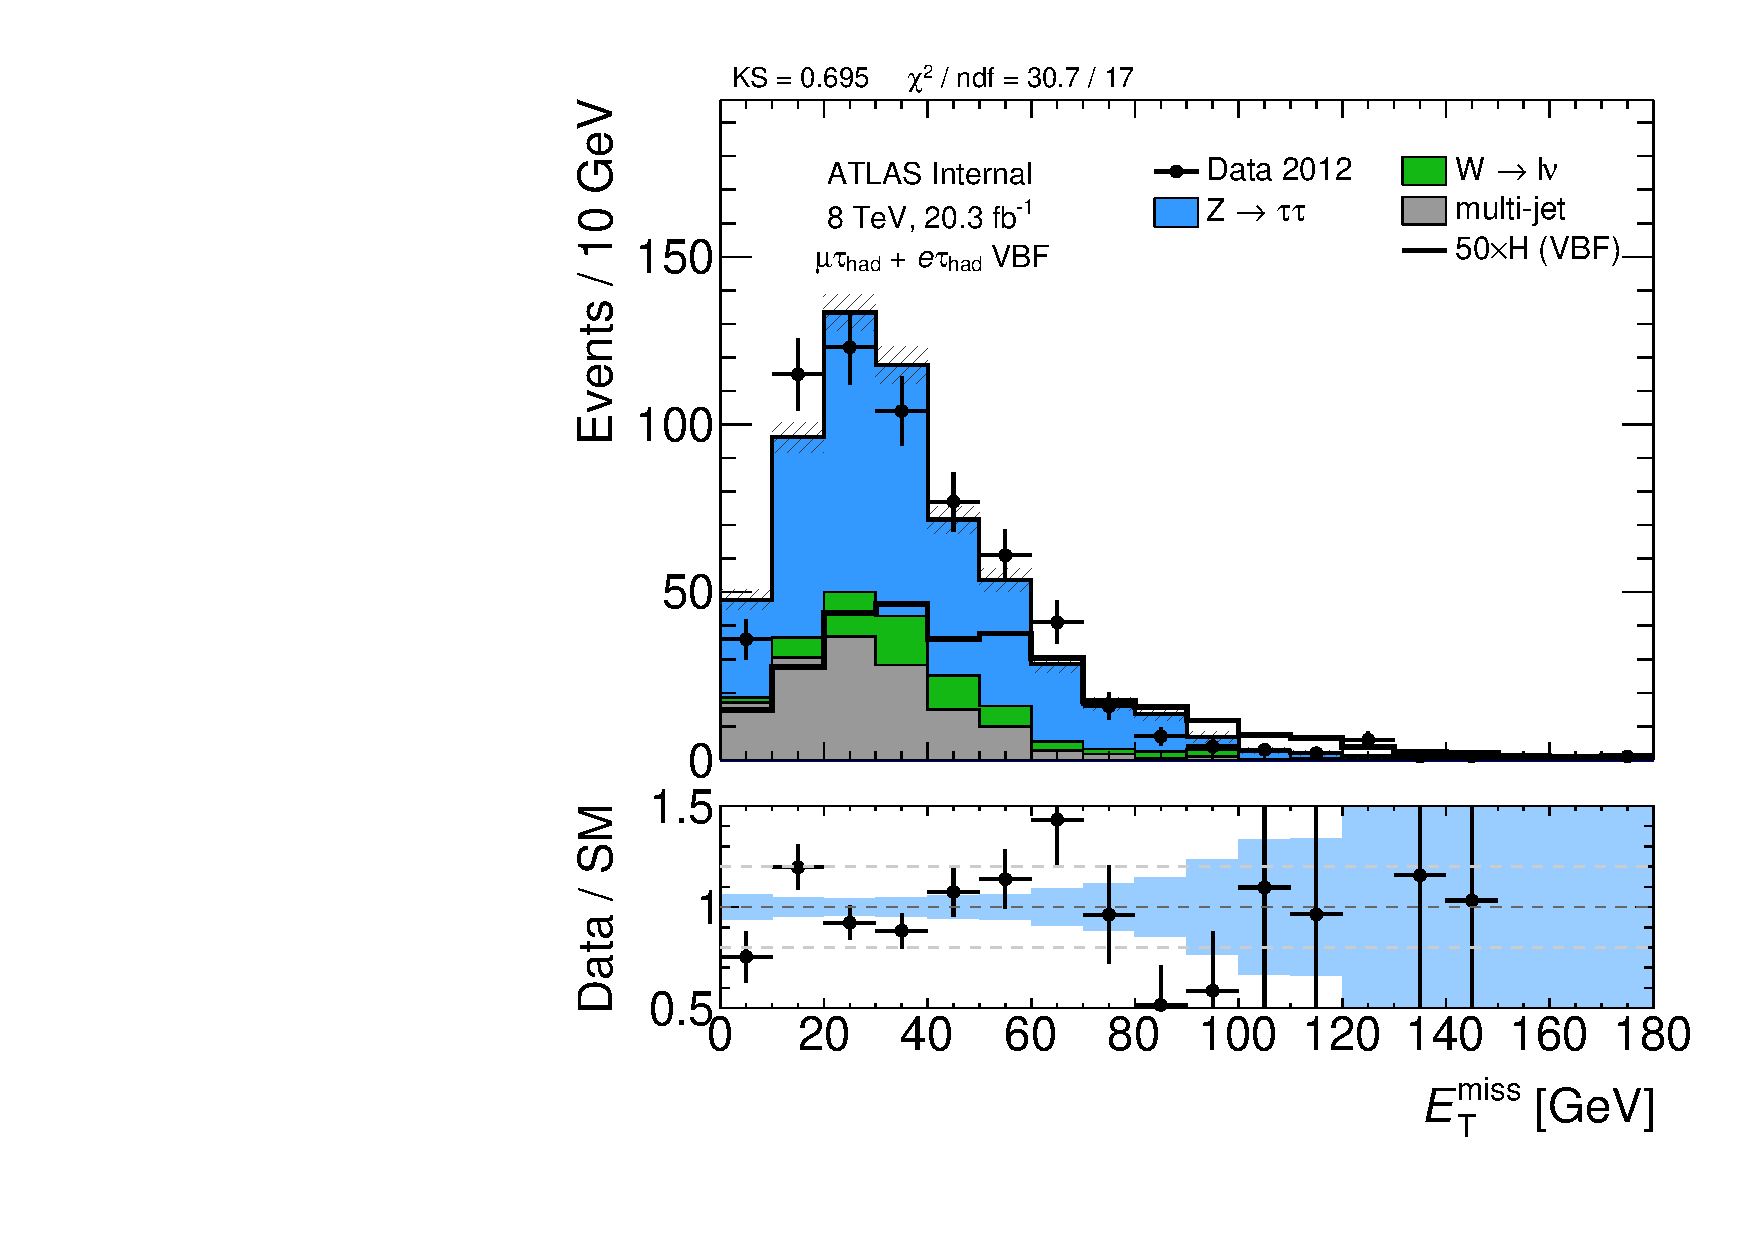
\includegraphics[width=0.32\textwidth]{figures/vbf-LTT/met-pt-hi}
  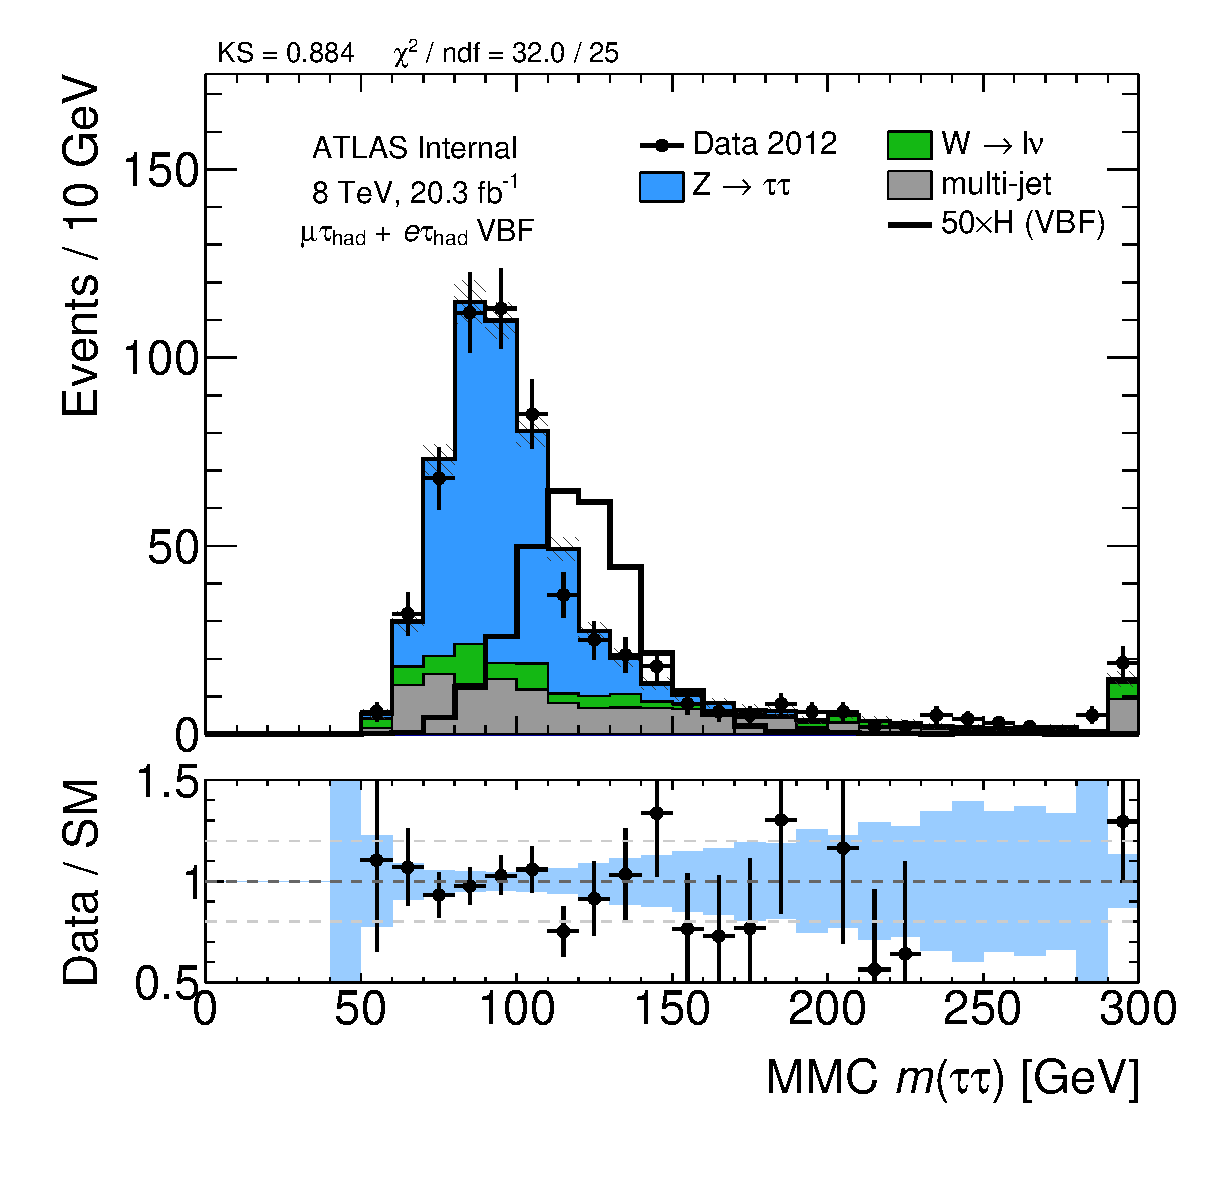
\includegraphics[width=0.32\textwidth]{figures/vbf-LTT/mMMC}
  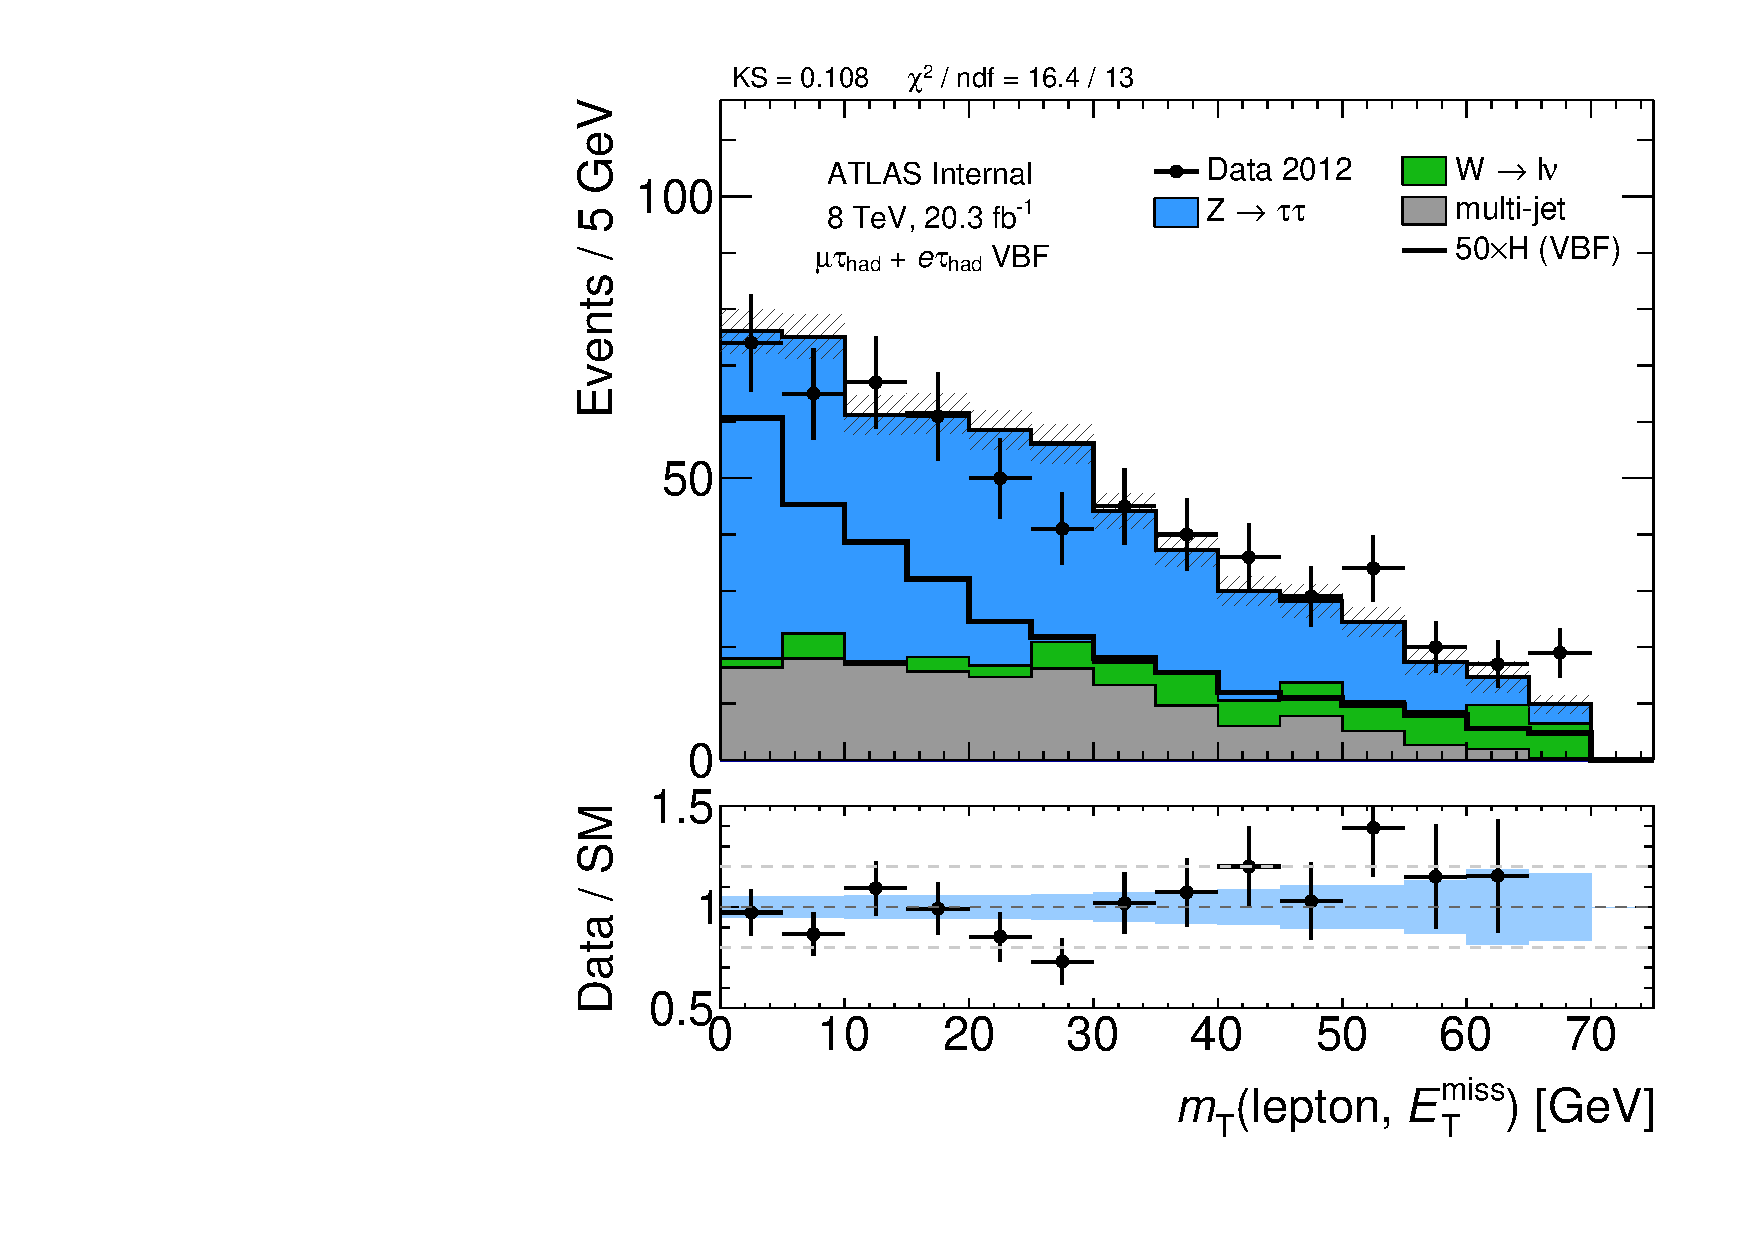
\includegraphics[width=0.32\textwidth]{figures/vbf-LTT/mT}
  % --------------
  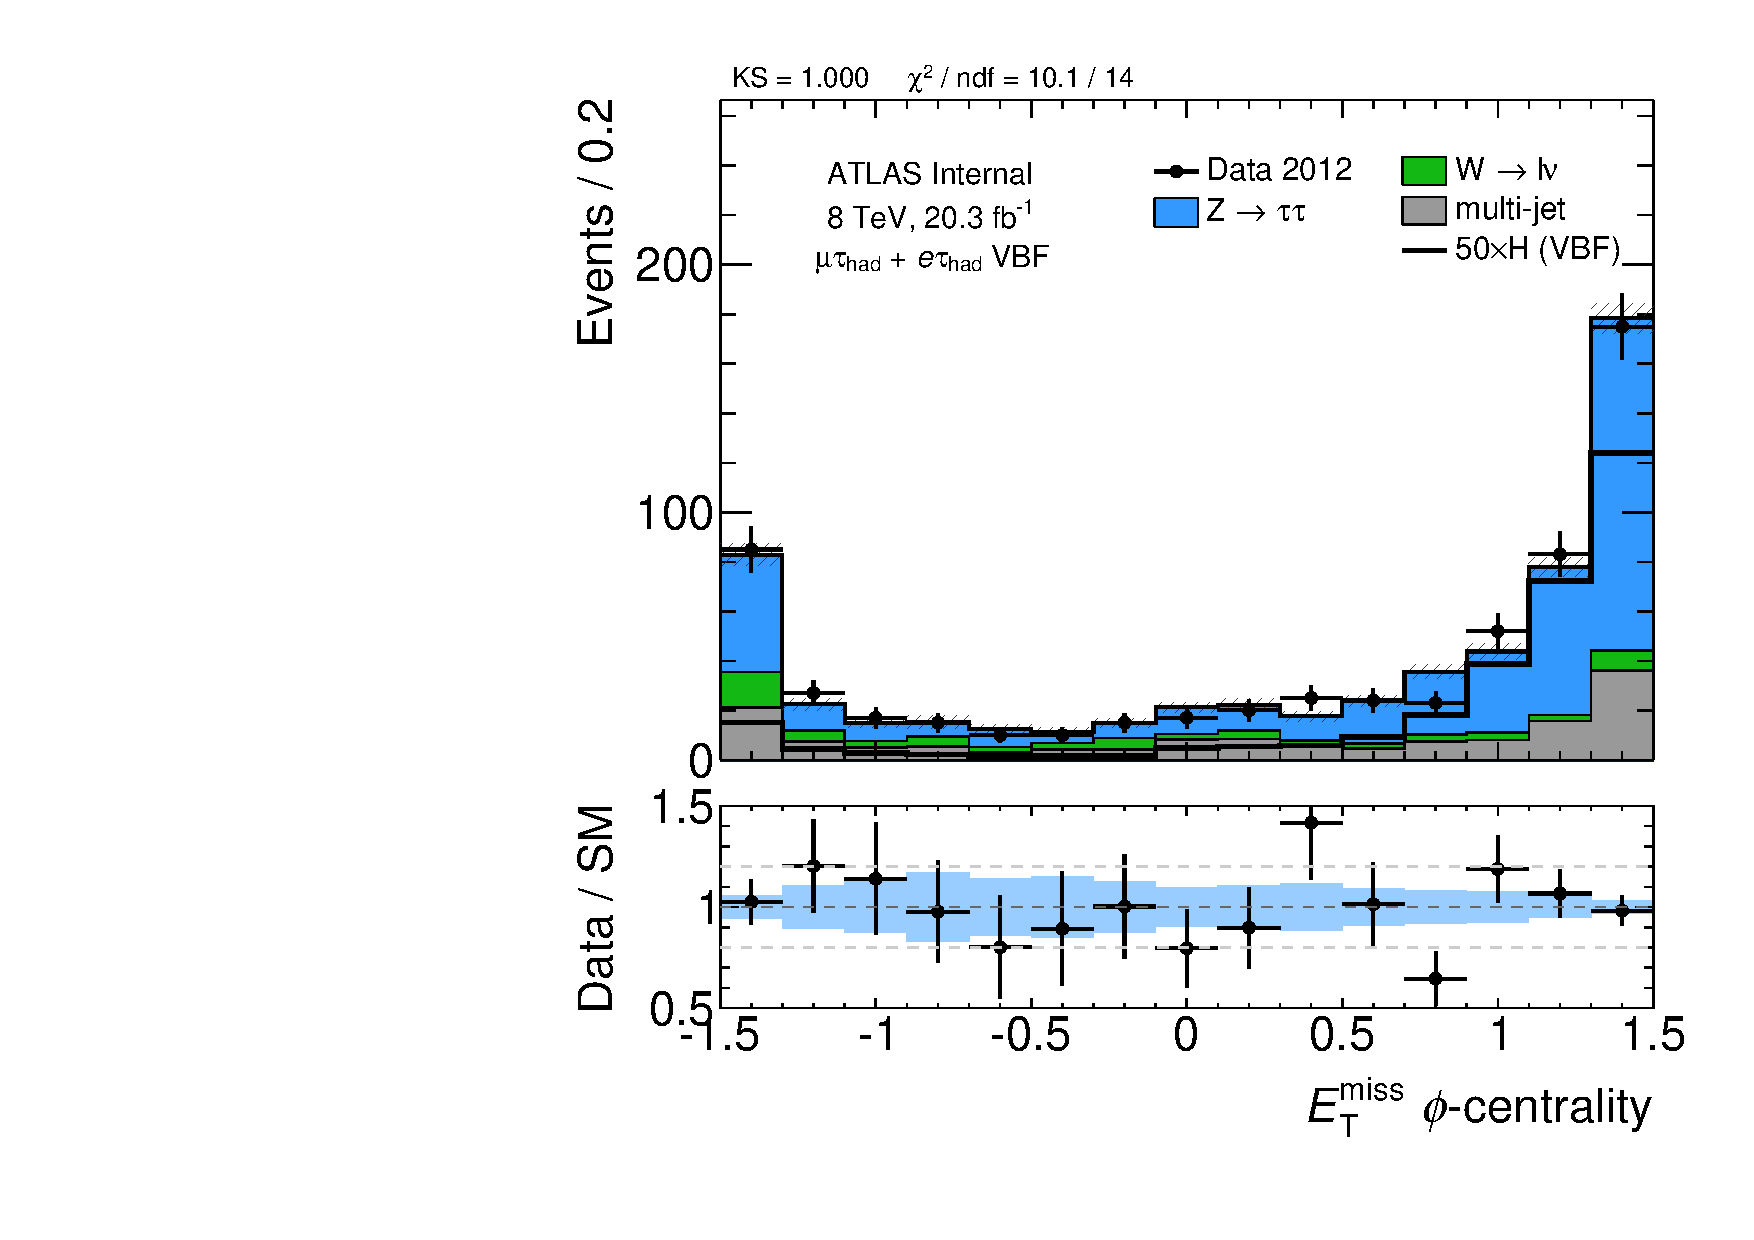
\includegraphics[width=0.32\textwidth]{figures/vbf-LTT/met-phi-centrality}
  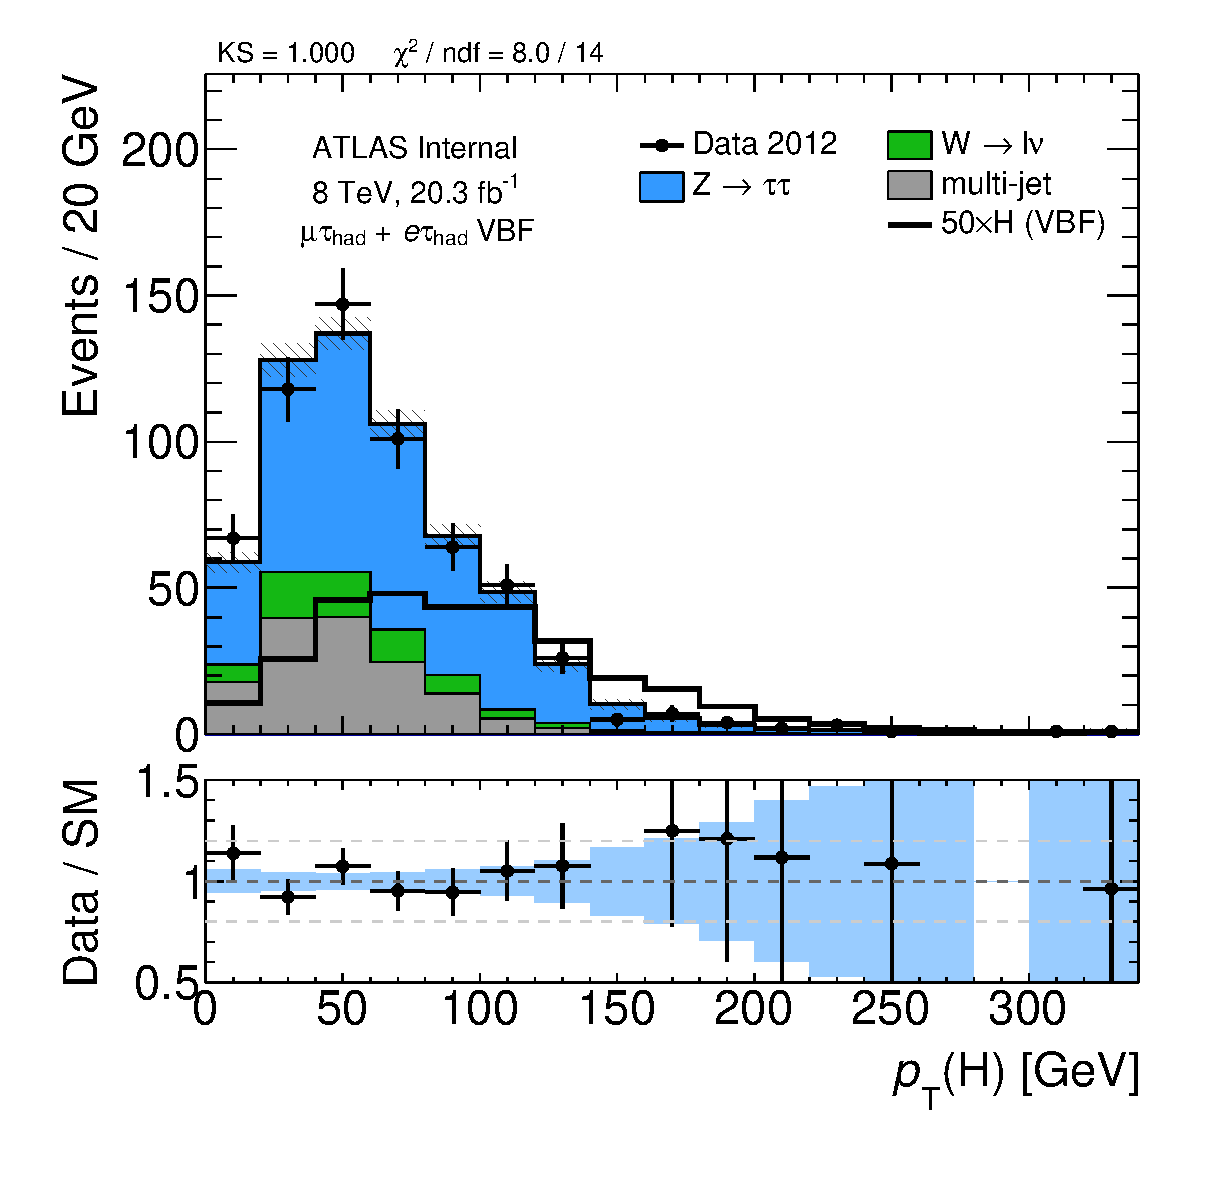
\includegraphics[width=0.32\textwidth]{figures/vbf-LTT/H-pt-hi}
  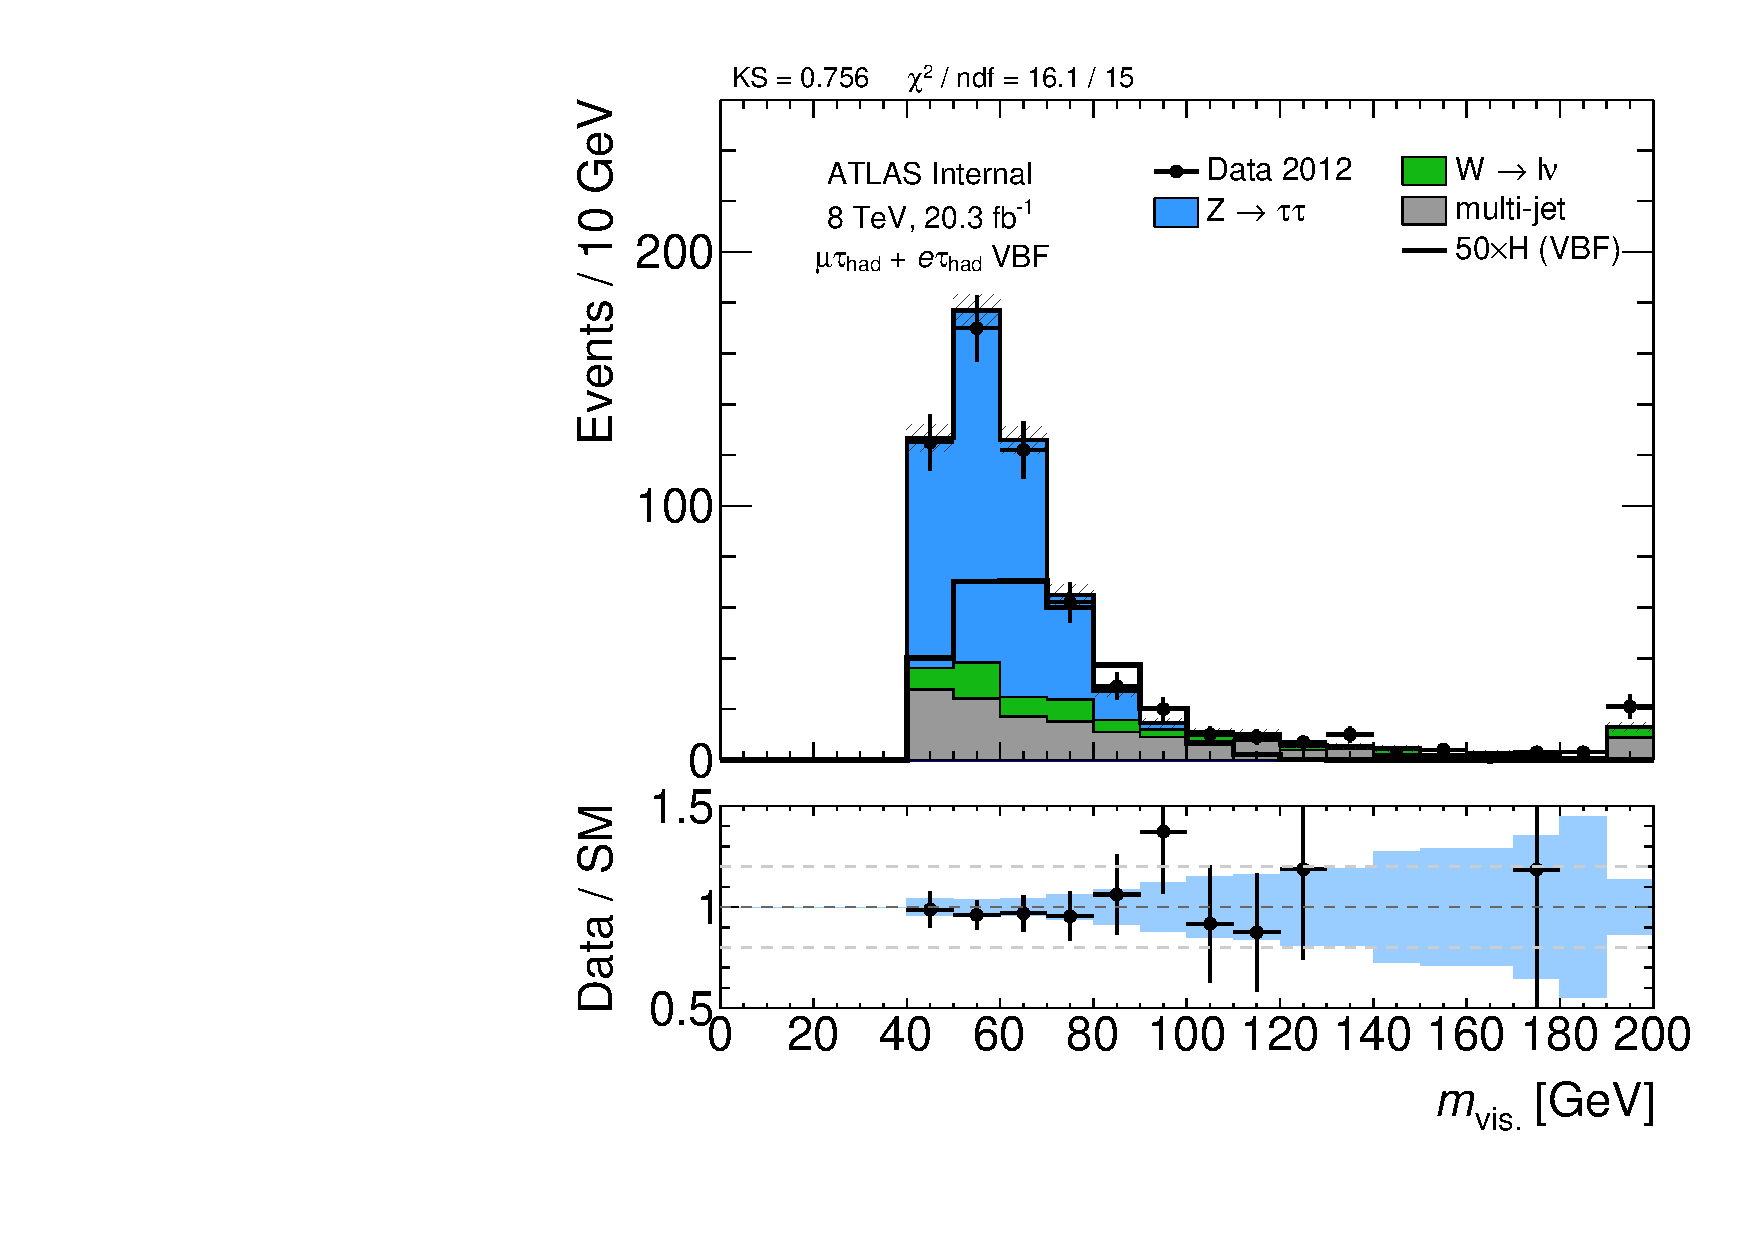
\includegraphics[width=0.32\textwidth]{figures/vbf-LTT/mvis}
  \caption{Variables.}
  \label{fig:prospects-ltt-taus}
\end{figure}

\begin{figure}[tp]
  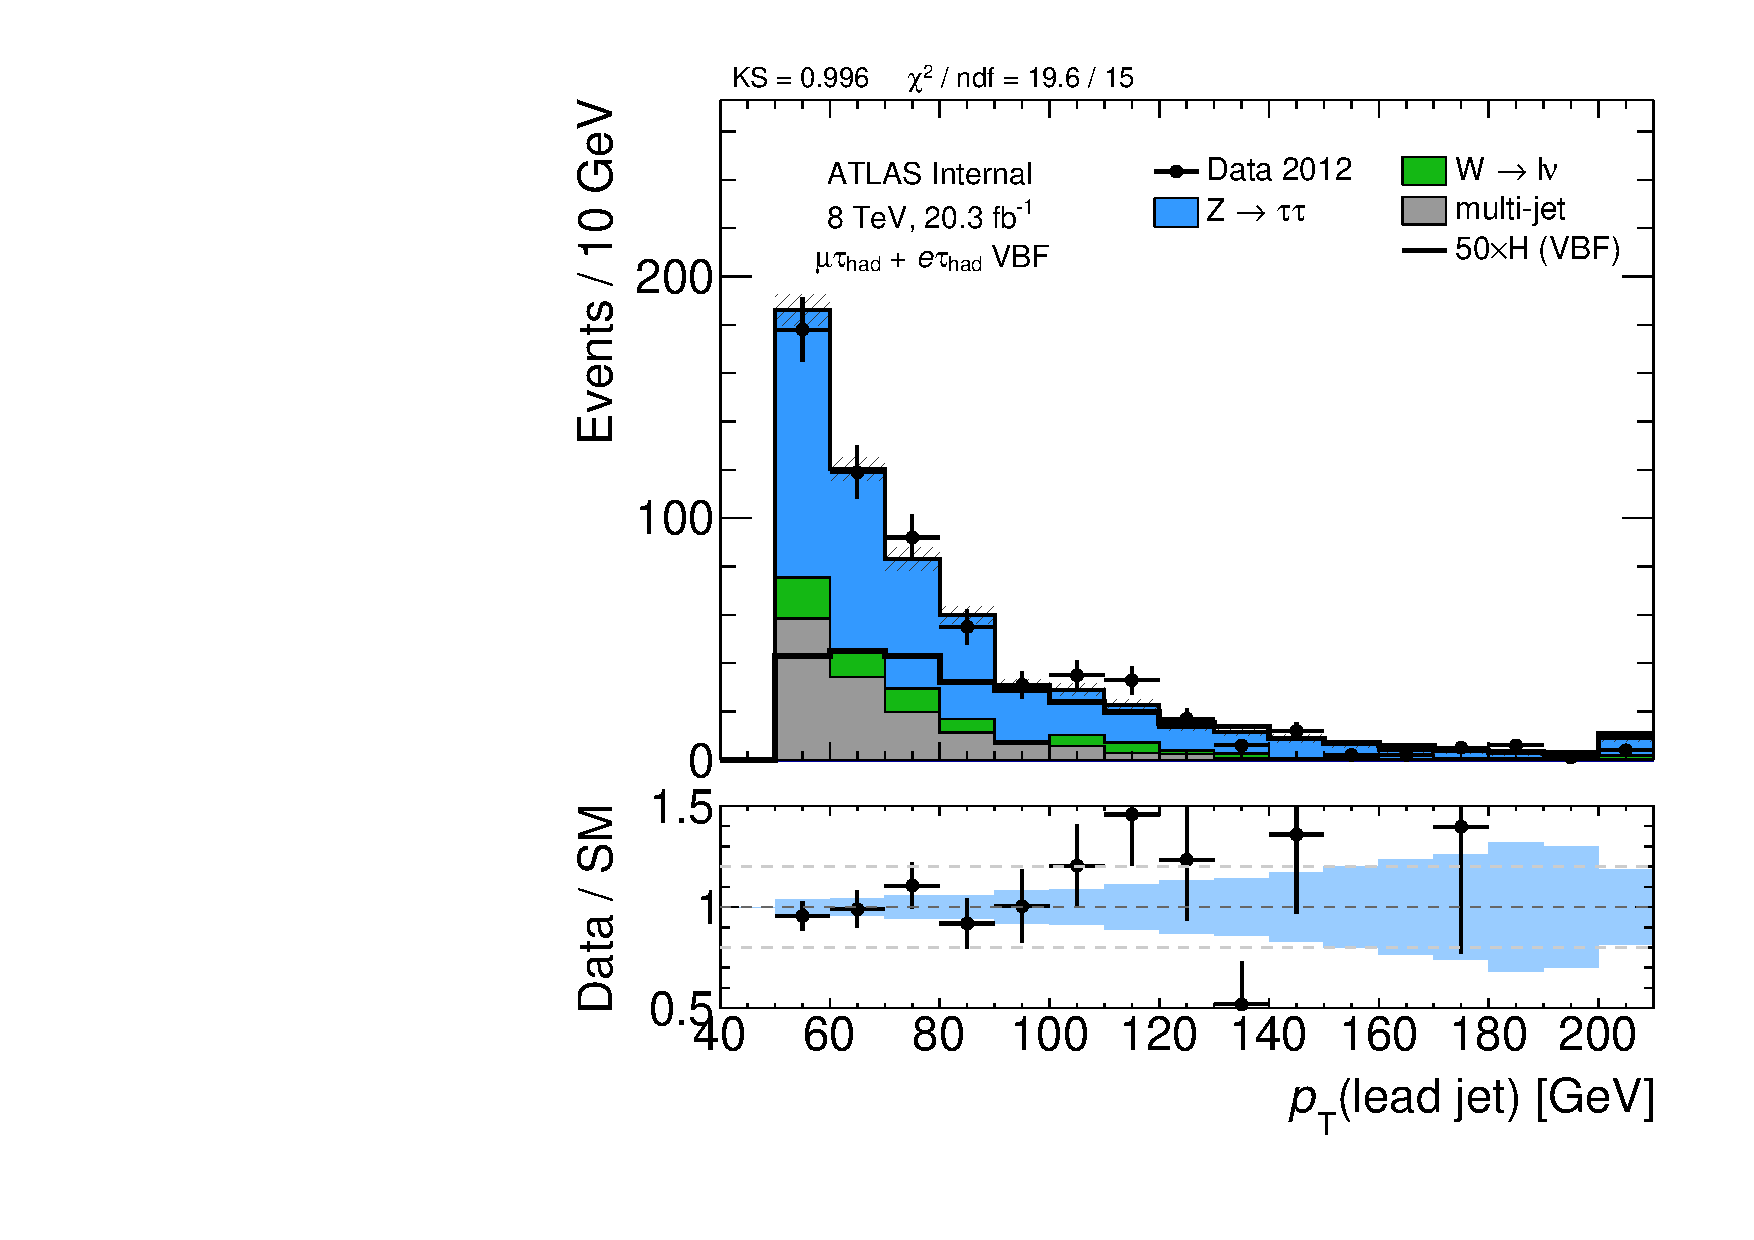
\includegraphics[width=0.32\textwidth]{figures/vbf-LTT/jet-1-pt}
  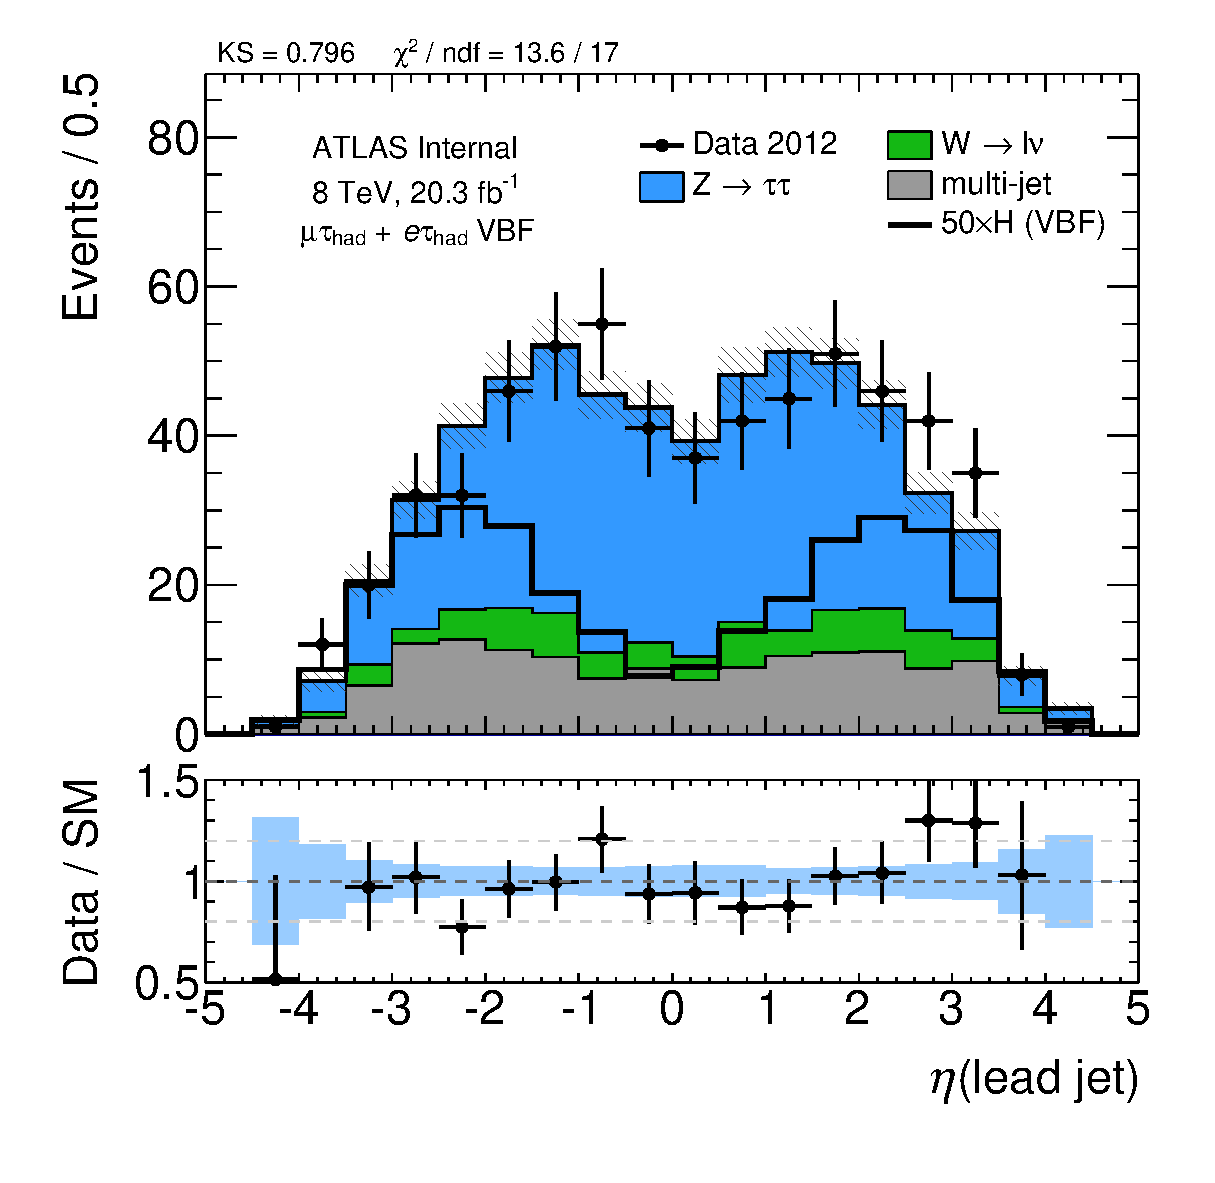
\includegraphics[width=0.32\textwidth]{figures/vbf-LTT/jet-1-eta}
  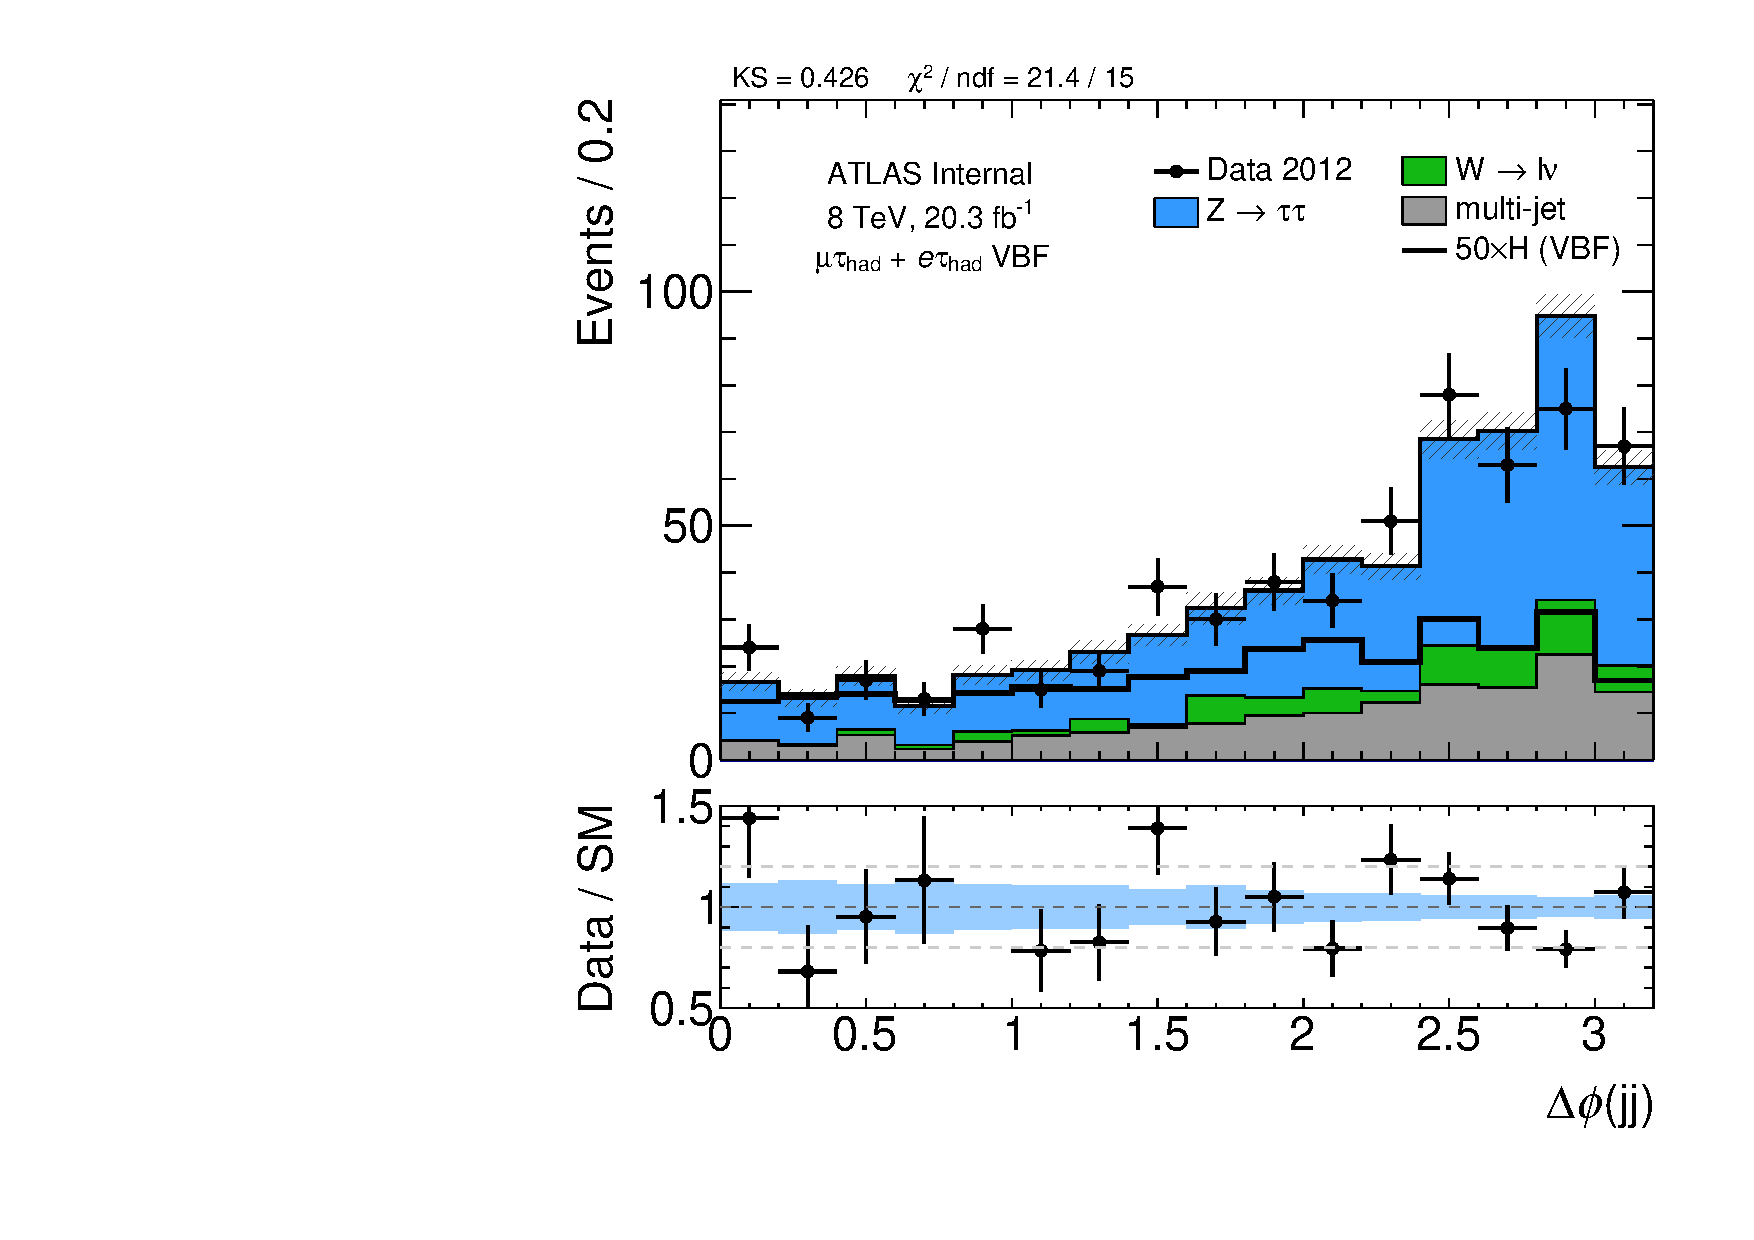
\includegraphics[width=0.32\textwidth]{figures/vbf-LTT/jets-dphi}
  % --------------
  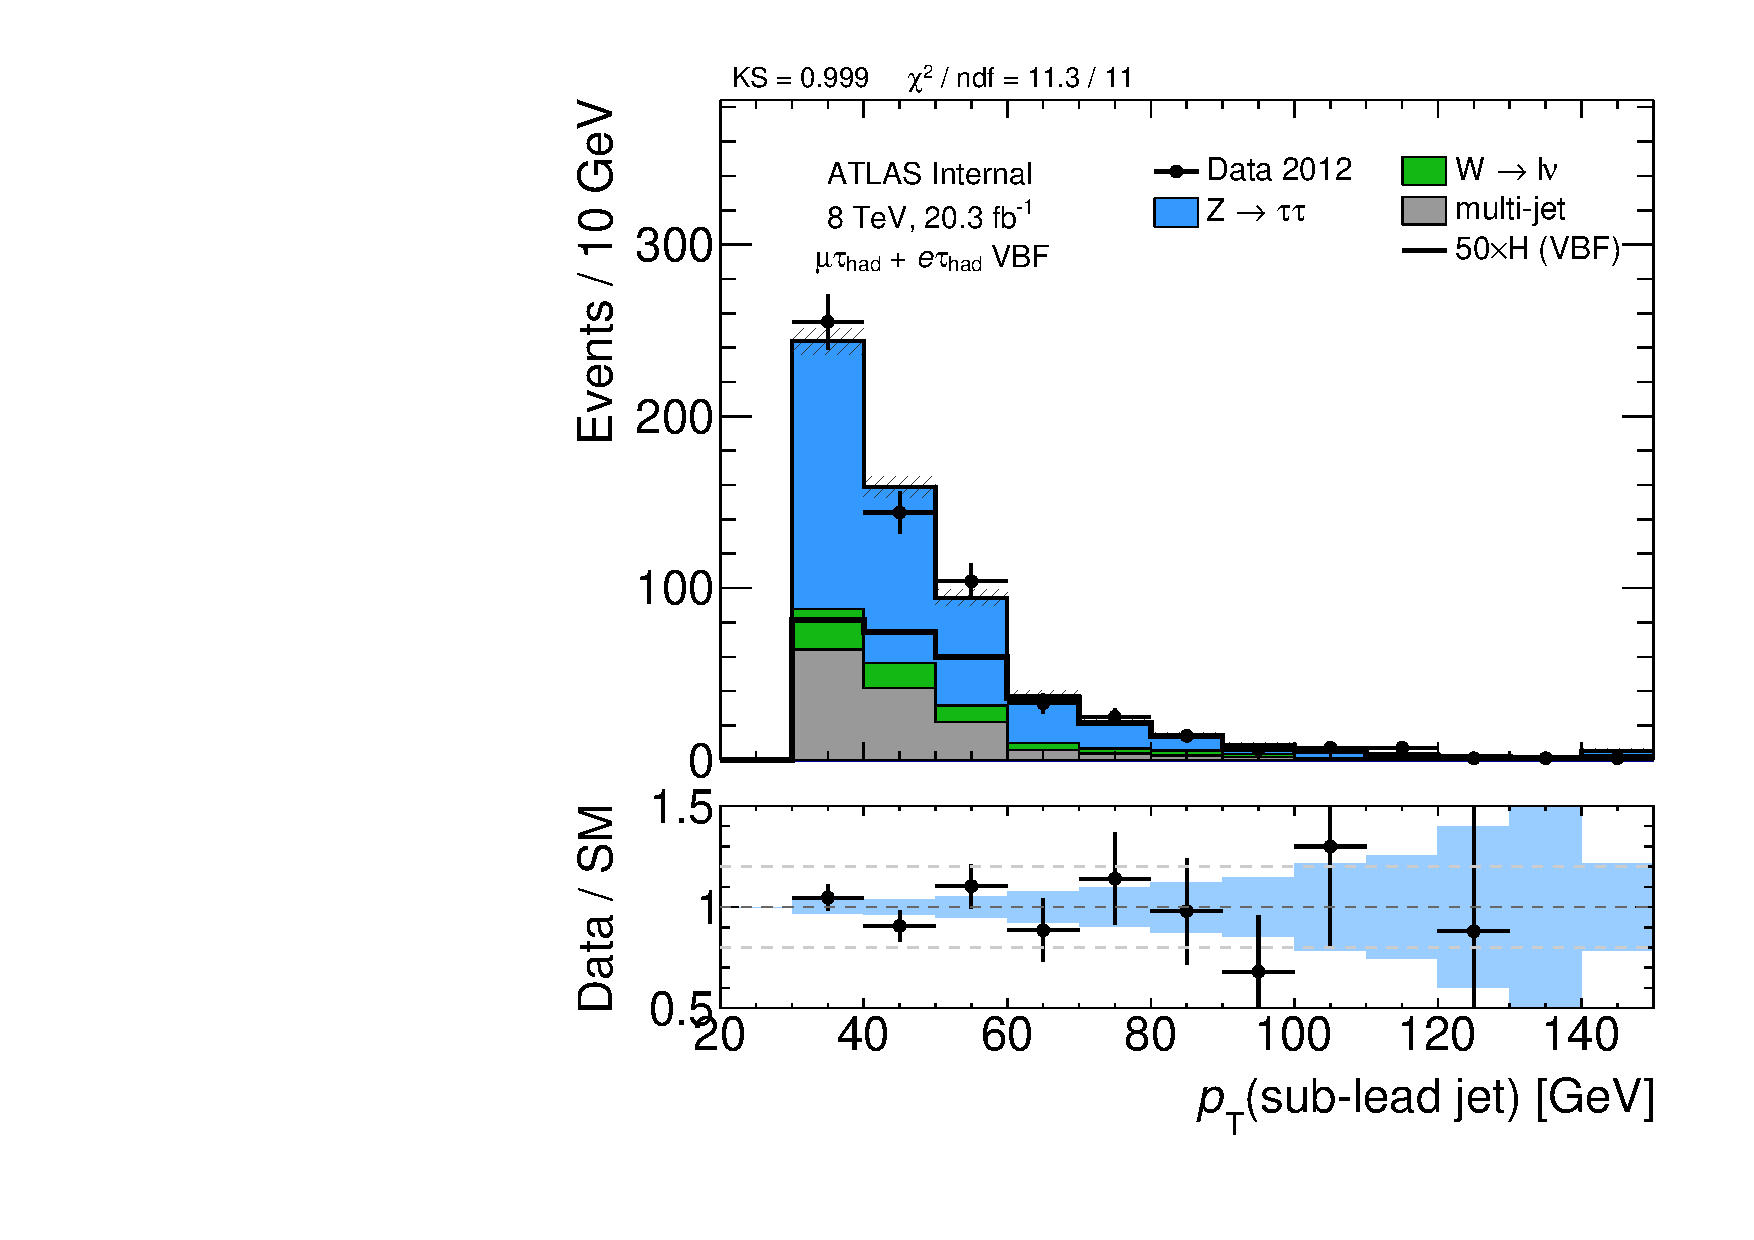
\includegraphics[width=0.32\textwidth]{figures/vbf-LTT/jet-2-pt}
  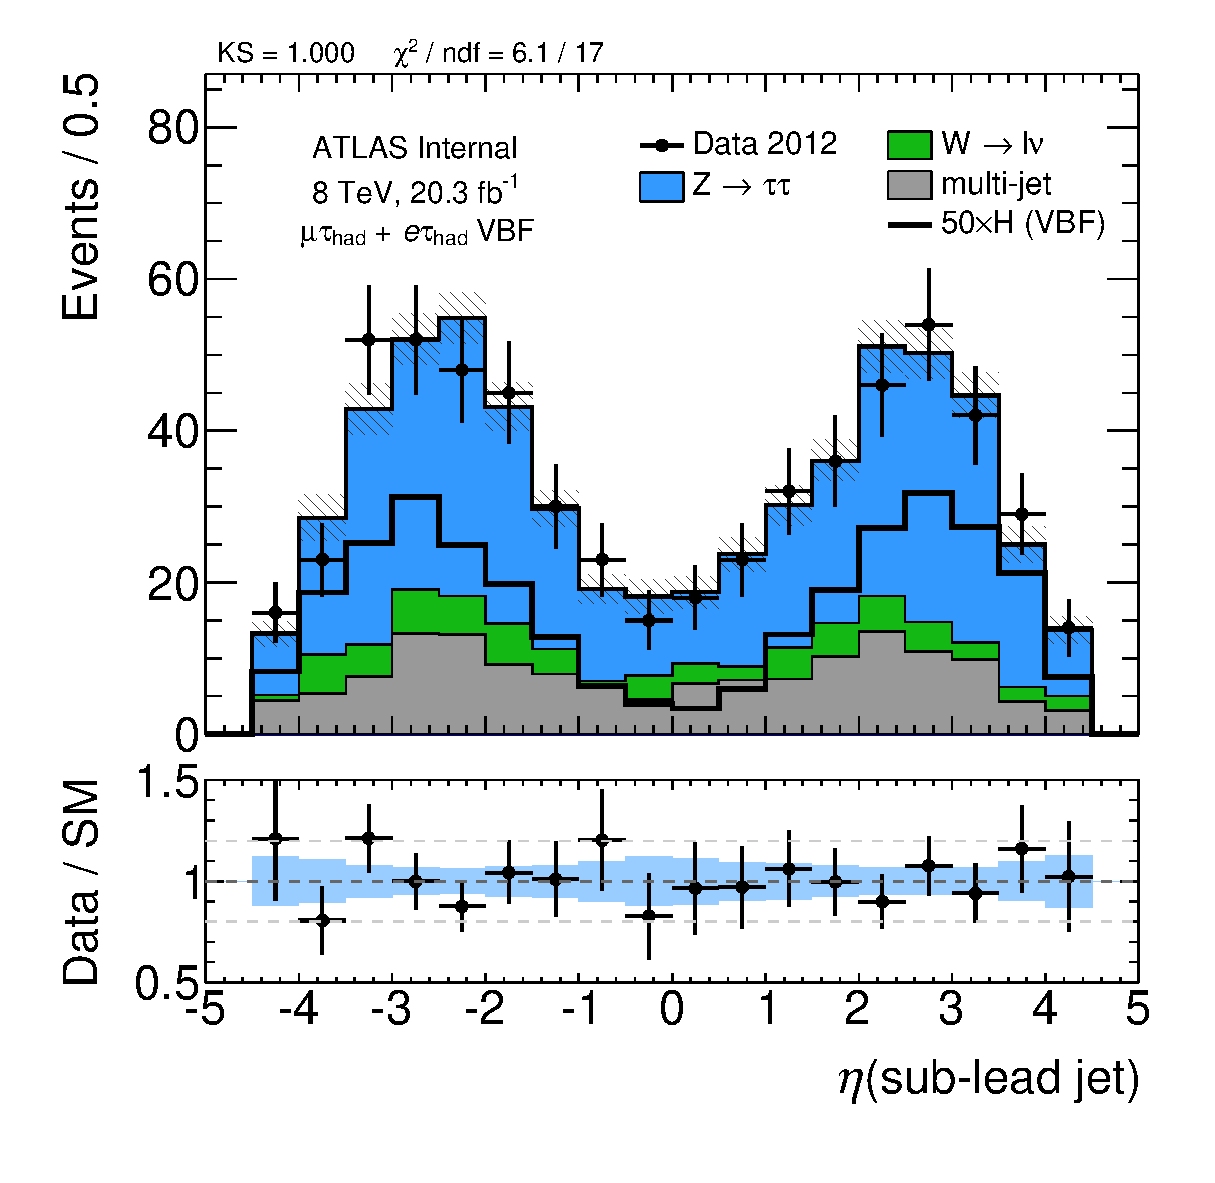
\includegraphics[width=0.32\textwidth]{figures/vbf-LTT/jet-2-eta}
  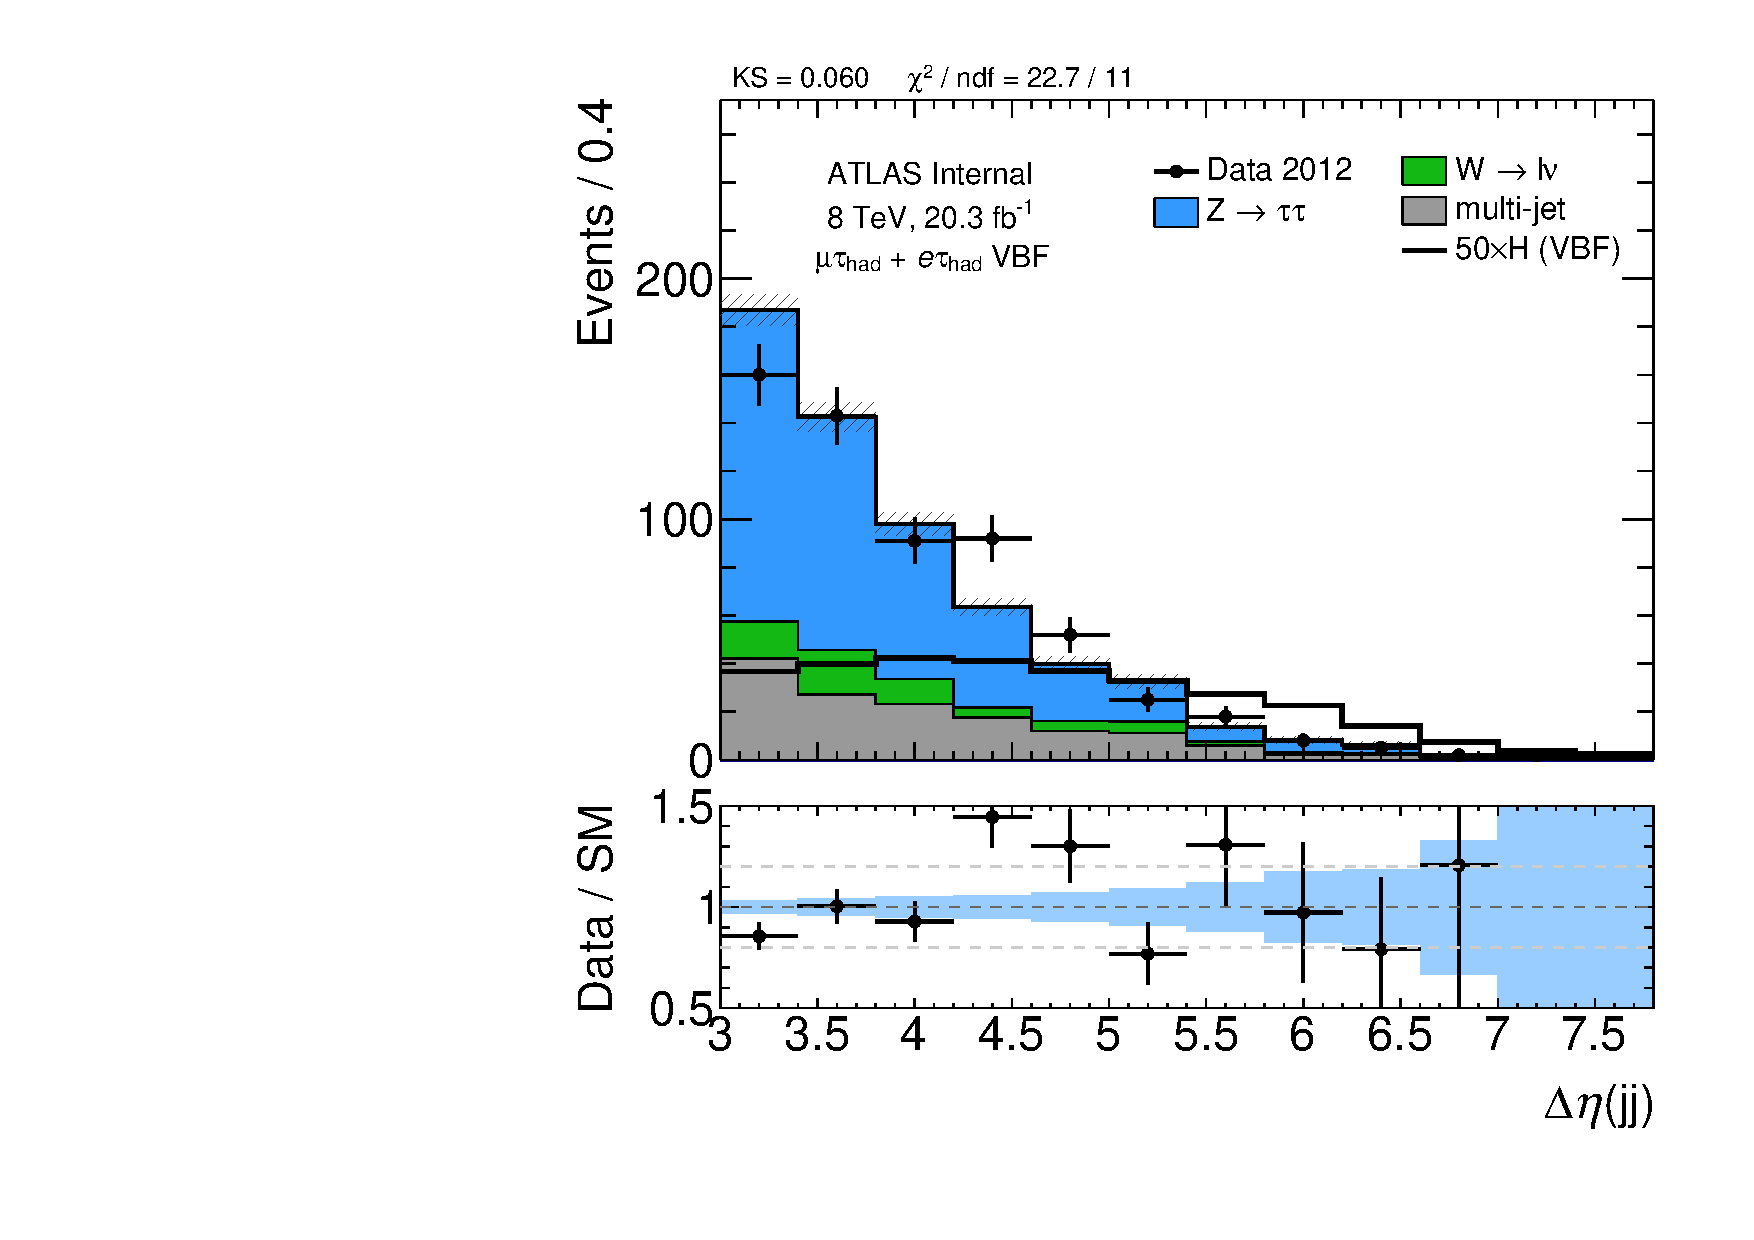
\includegraphics[width=0.32\textwidth]{figures/vbf-LTT/jets-deta}
  % --------------
  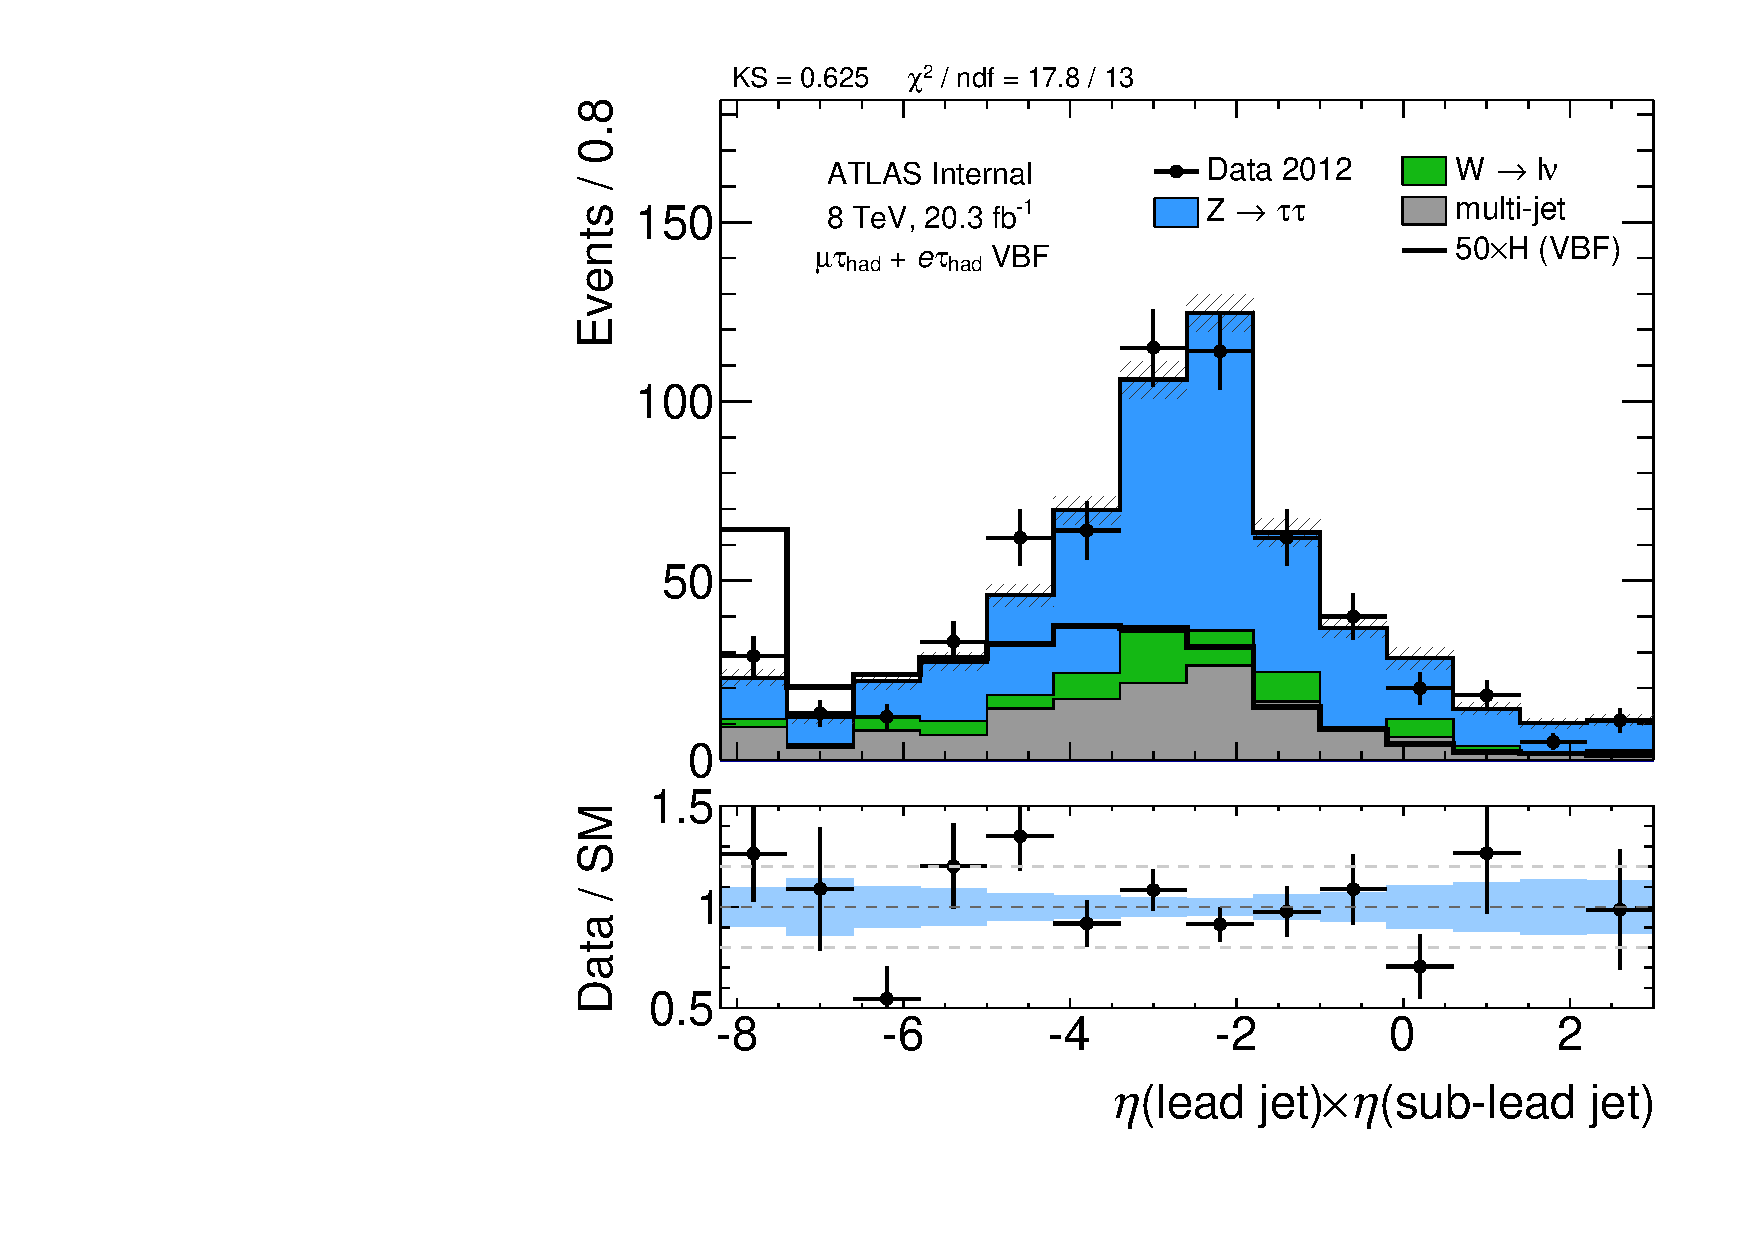
\includegraphics[width=0.32\textwidth]{figures/vbf-LTT/jets-etaprod}
  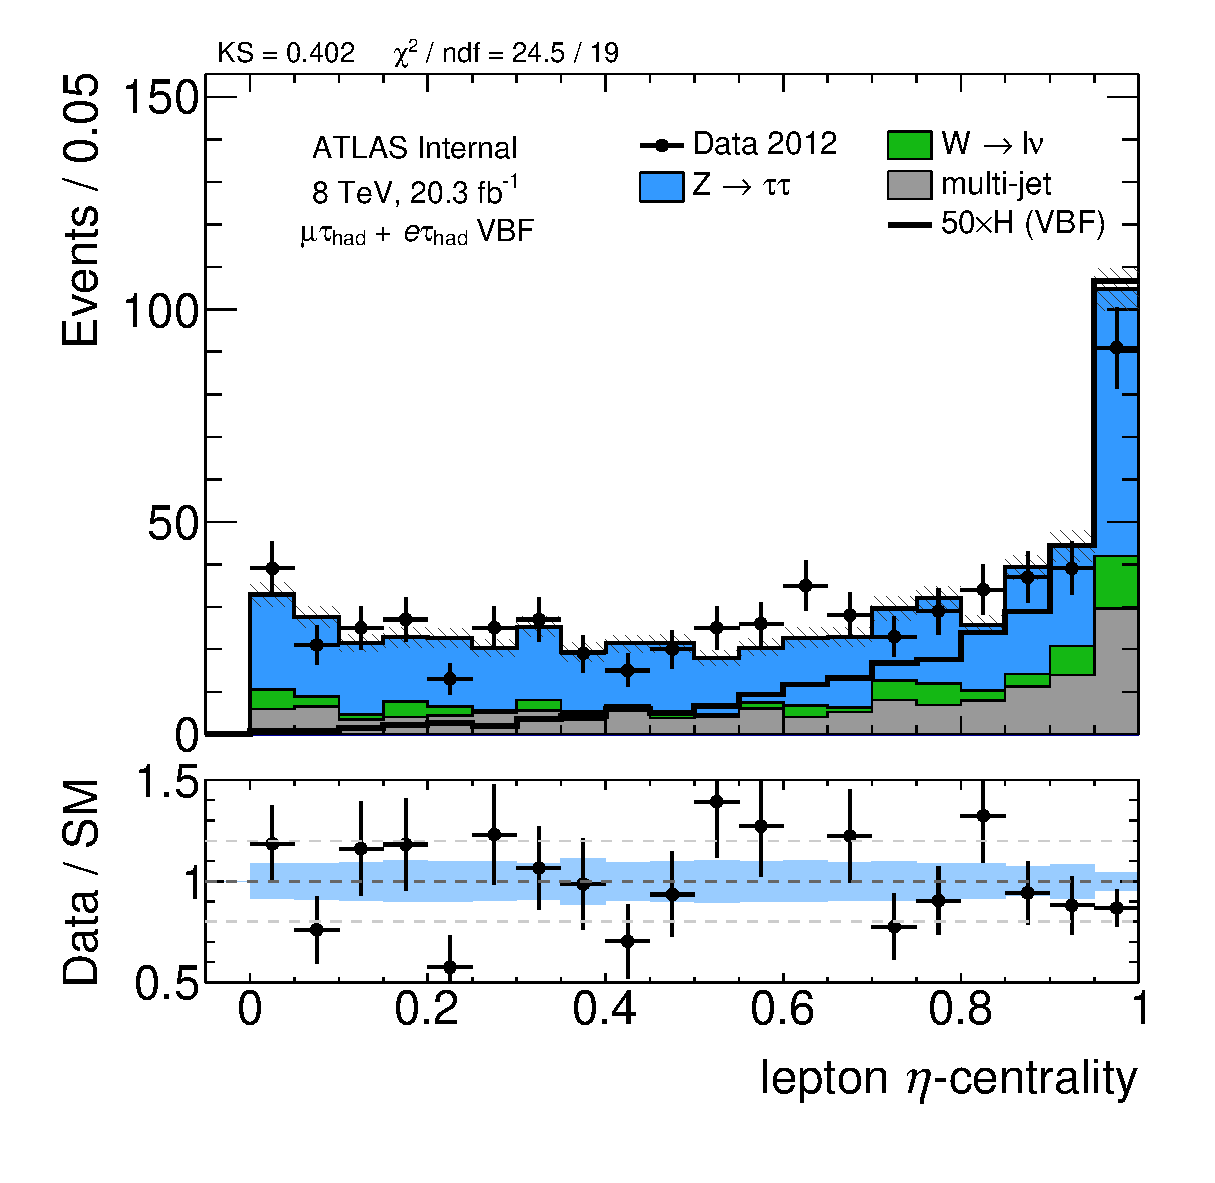
\includegraphics[width=0.32\textwidth]{figures/vbf-LTT/lep-eta-centrality}
  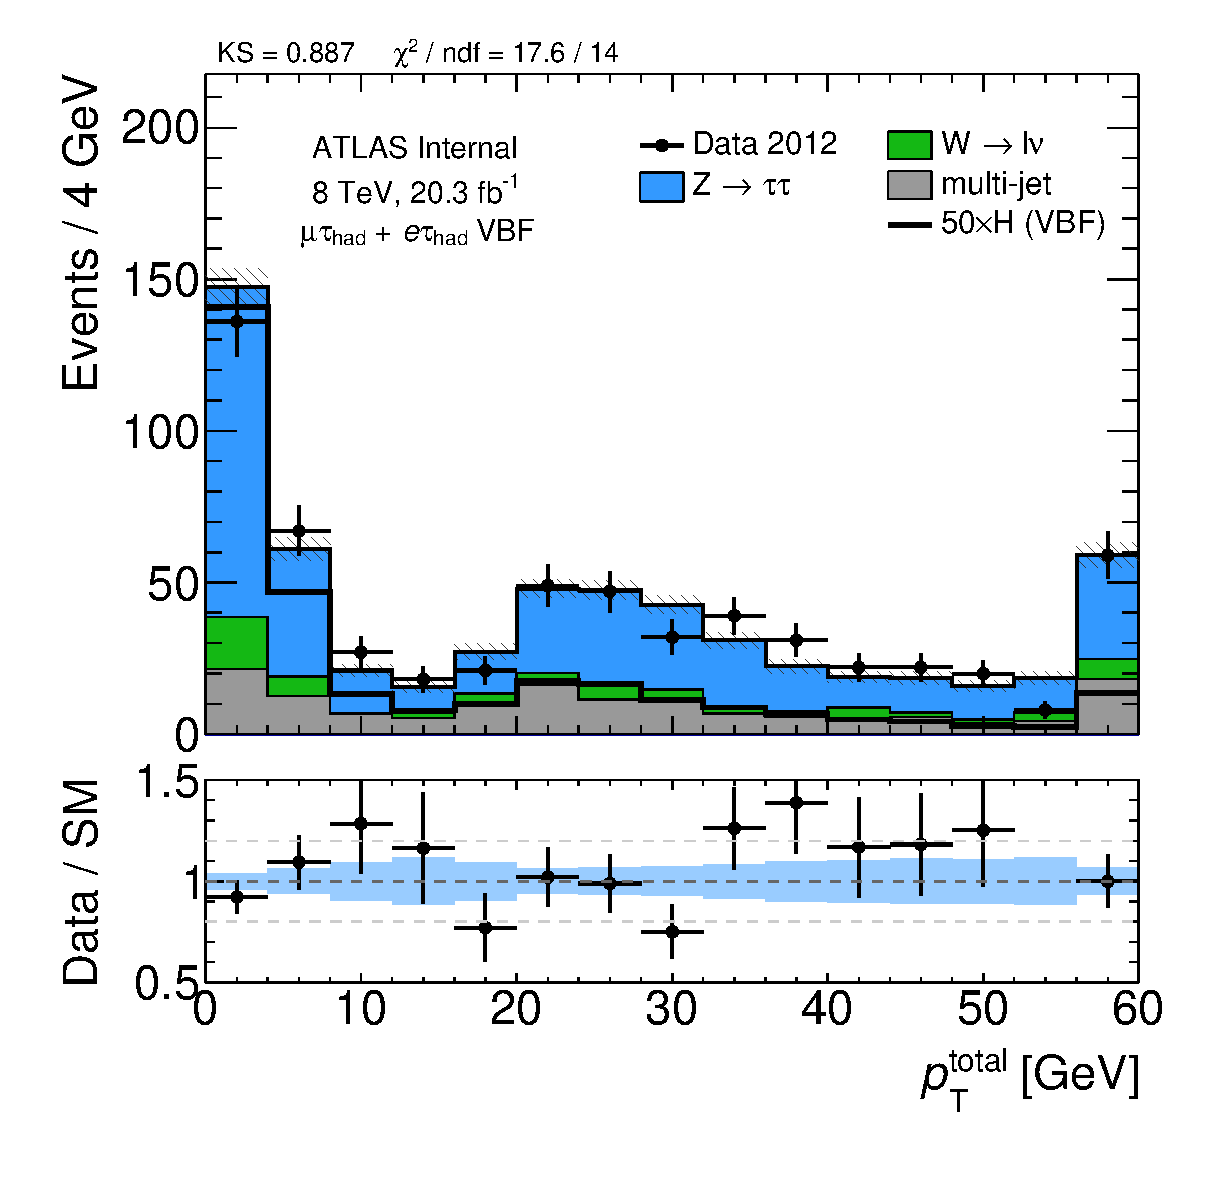
\includegraphics[width=0.32\textwidth]{figures/vbf-LTT/system-pt}
  % --------------
  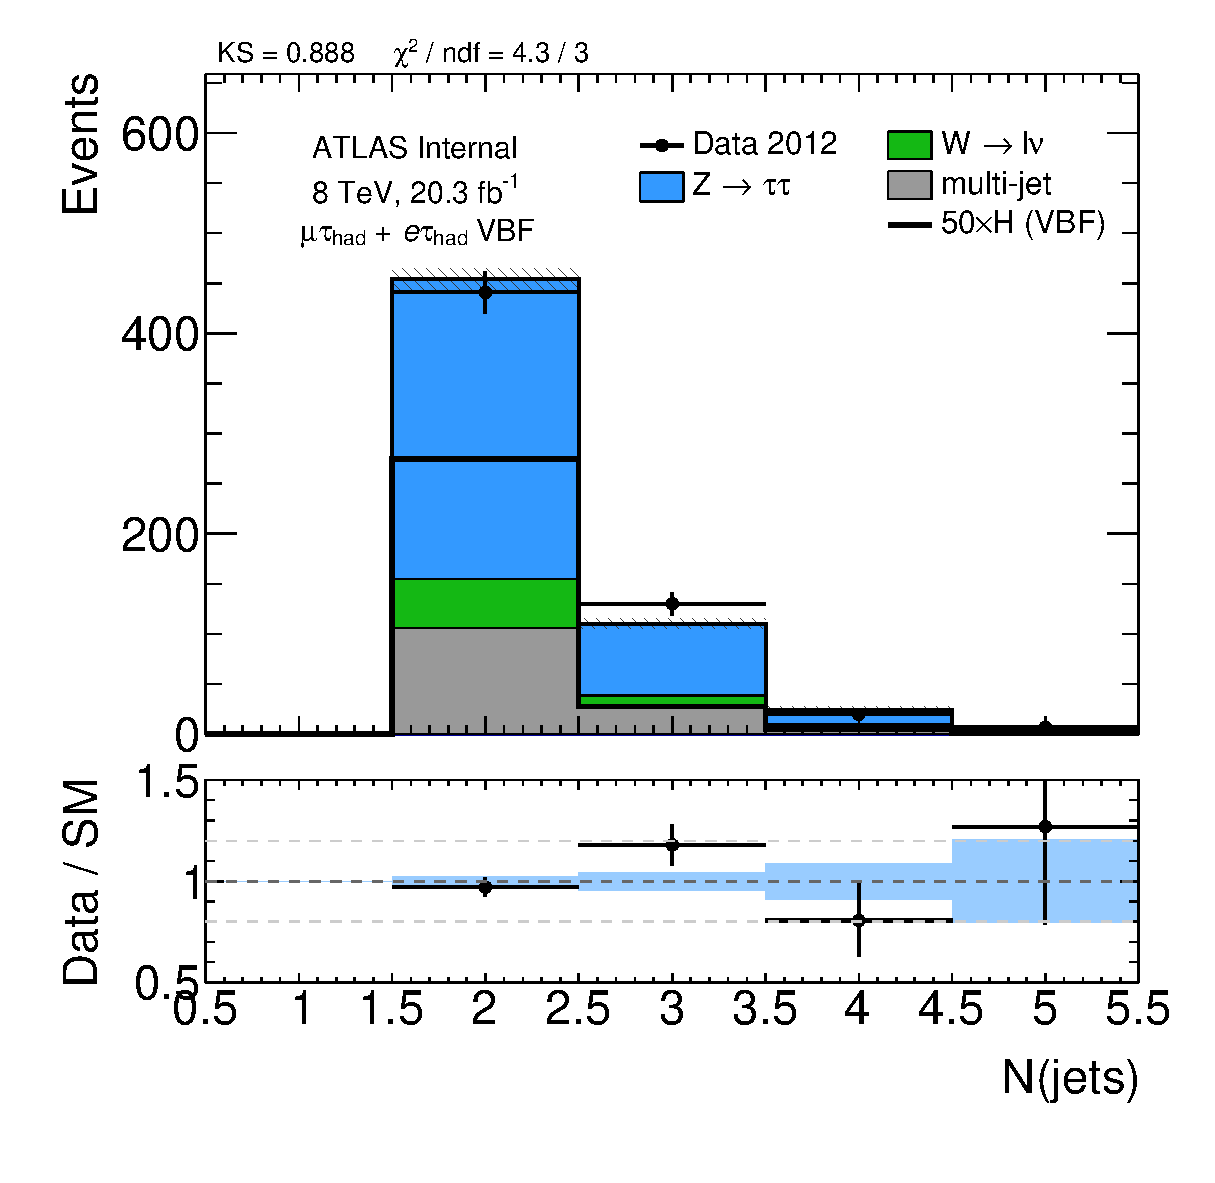
\includegraphics[width=0.32\textwidth]{figures/vbf-LTT/n-jets30}
  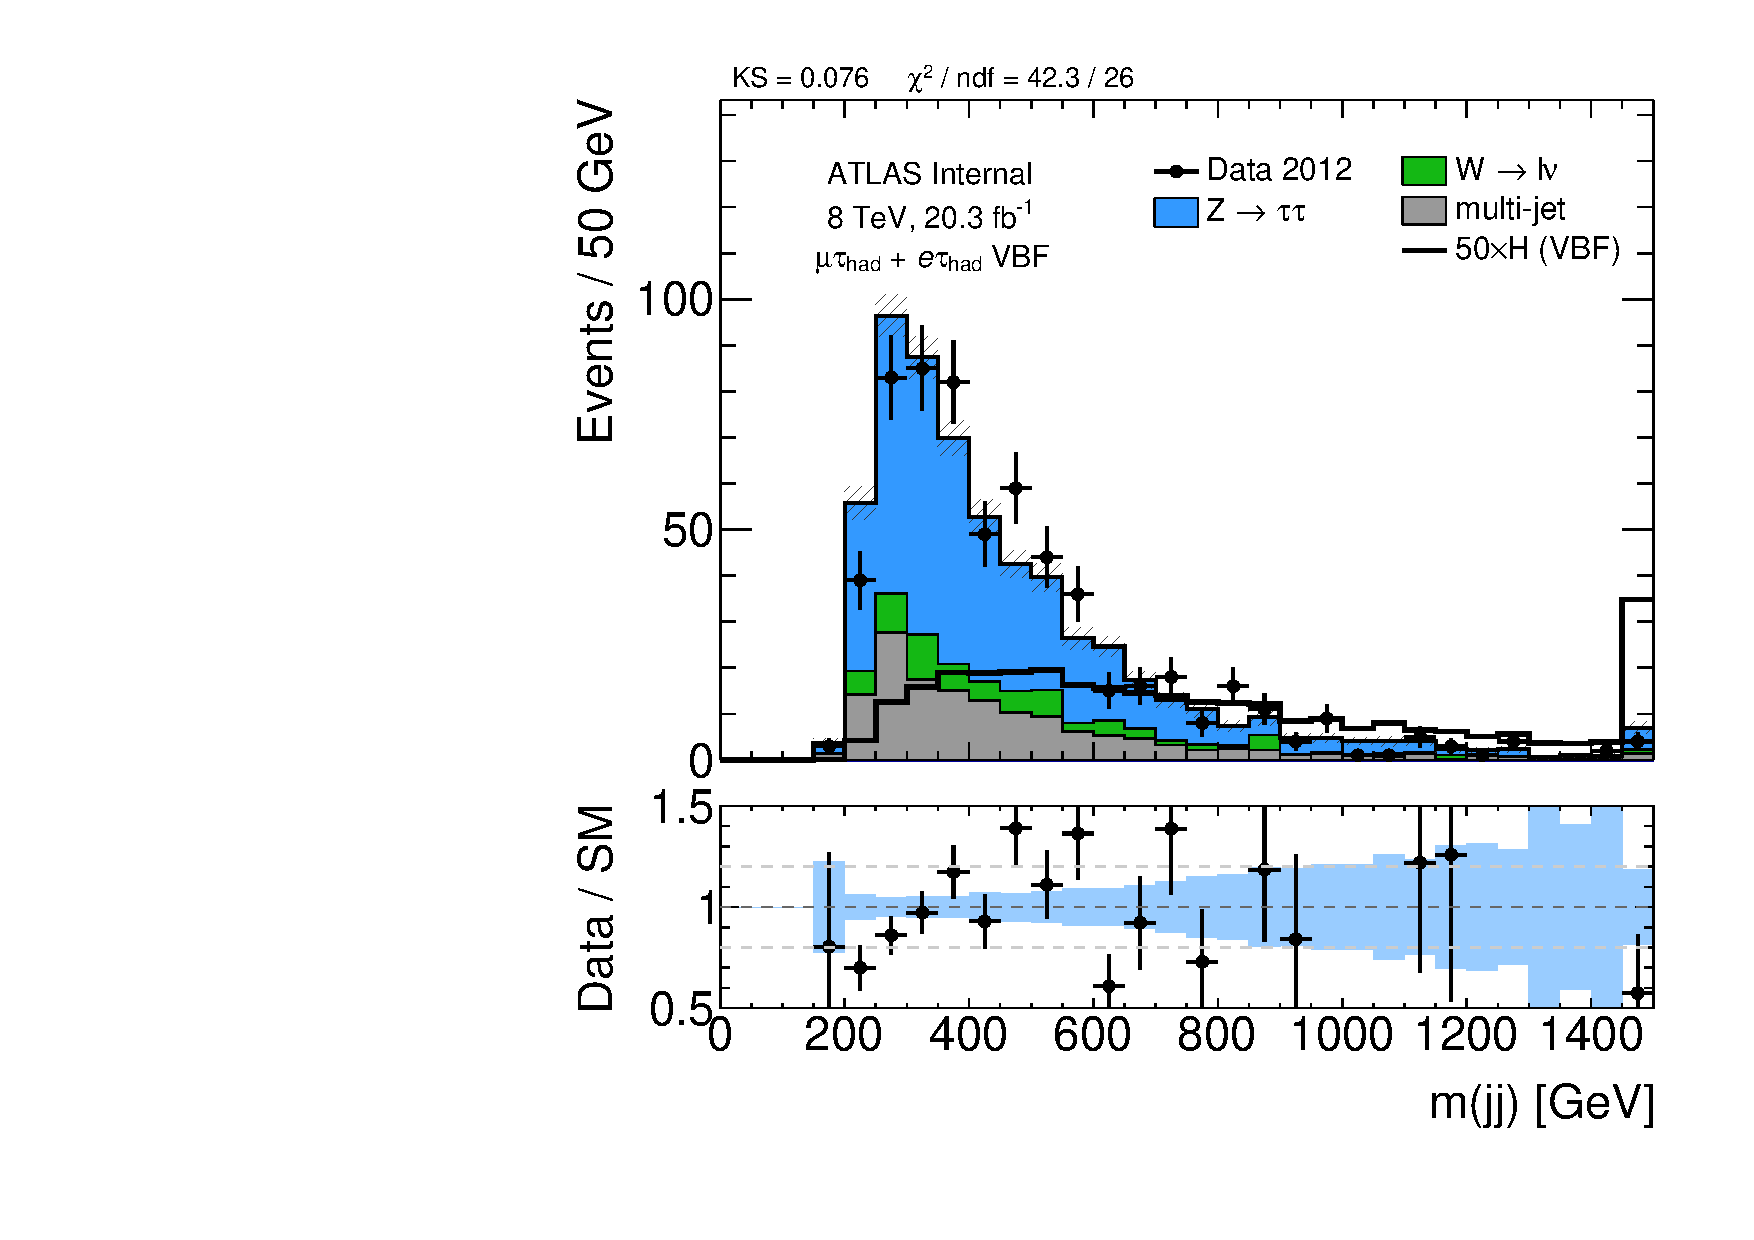
\includegraphics[width=0.32\textwidth]{figures/vbf-LTT/dijet-m-high}
  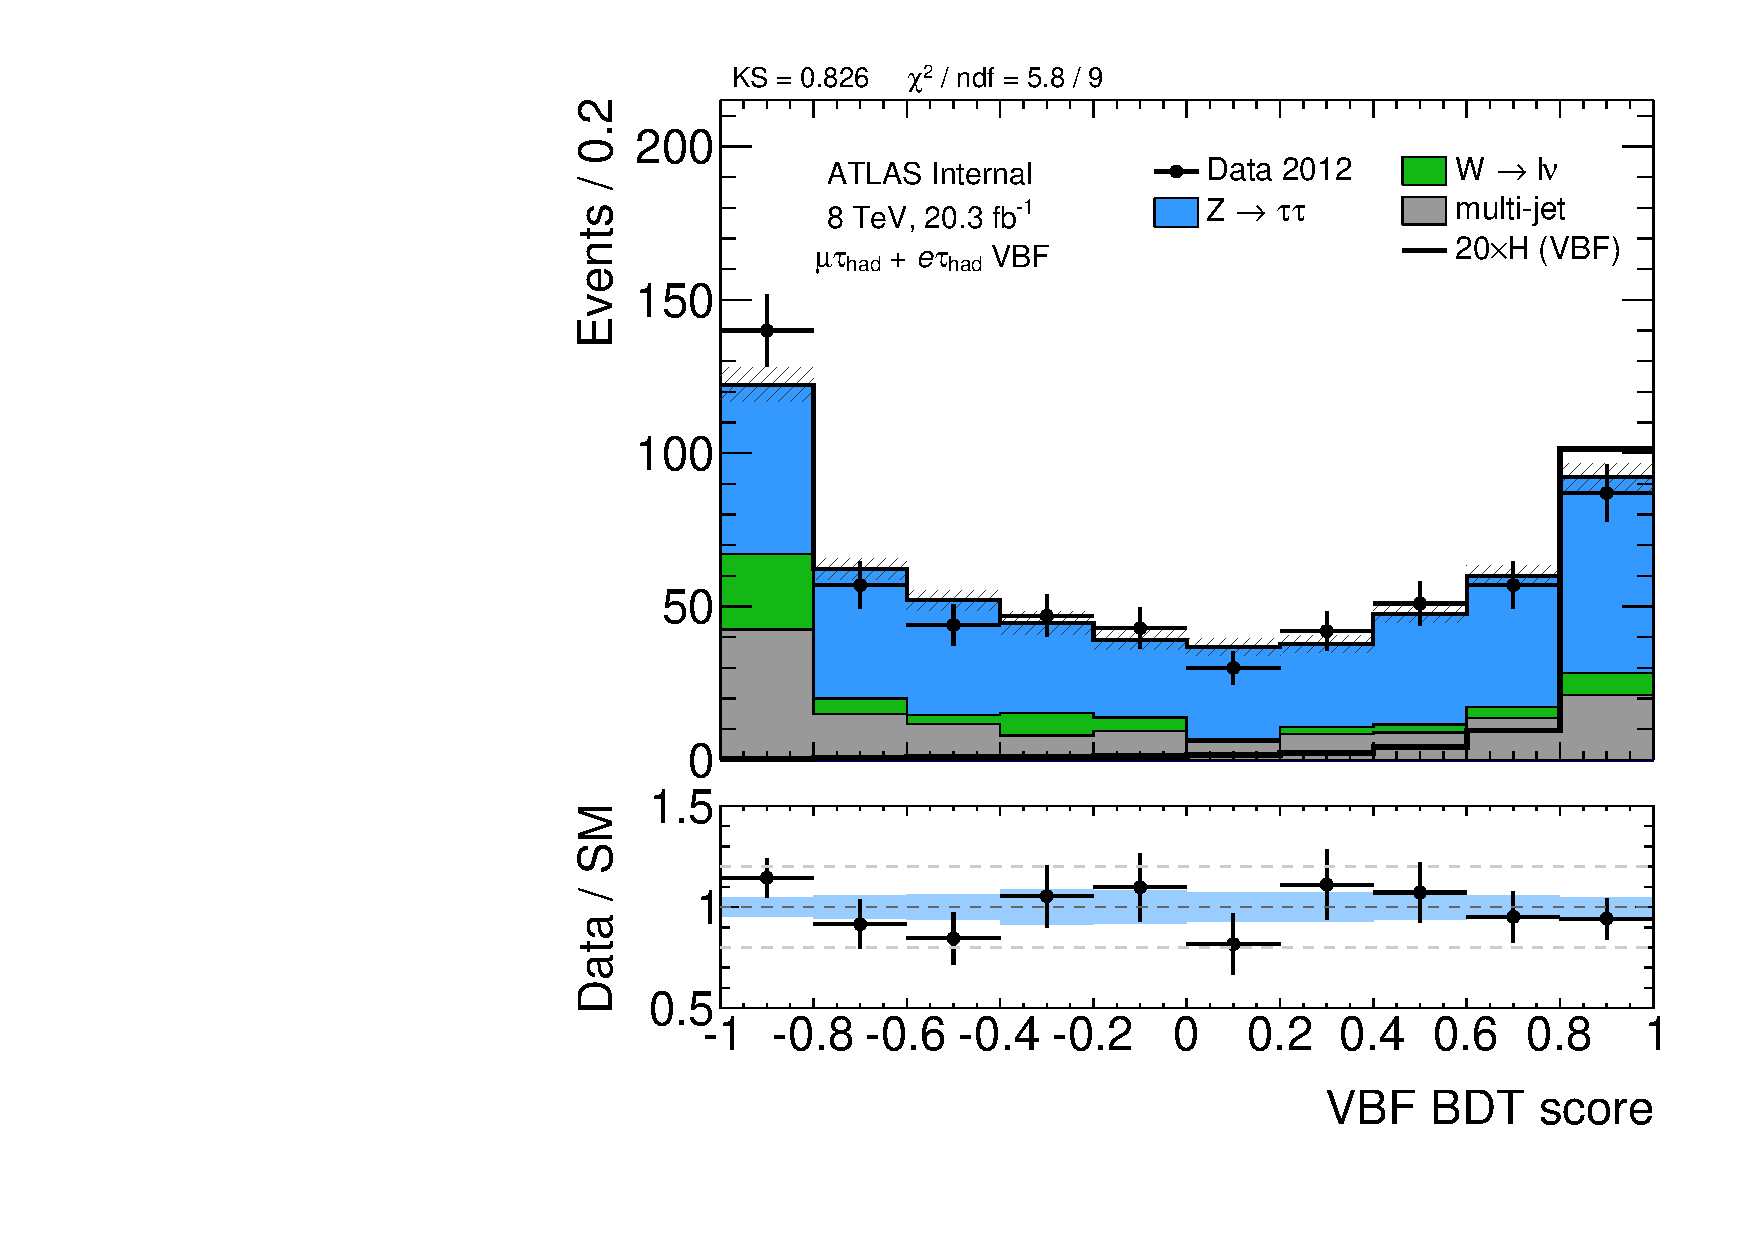
\includegraphics[width=0.32\textwidth]{figures/vbf-LTT/BDTEve-VBF}
  \caption{Variables.}
  \label{fig:prospects-ltt-jets}
\end{figure}

\section{HL-LHC}
\label{sec:prospects-hllhc}

\begin{figure}[tp]
  \centering
  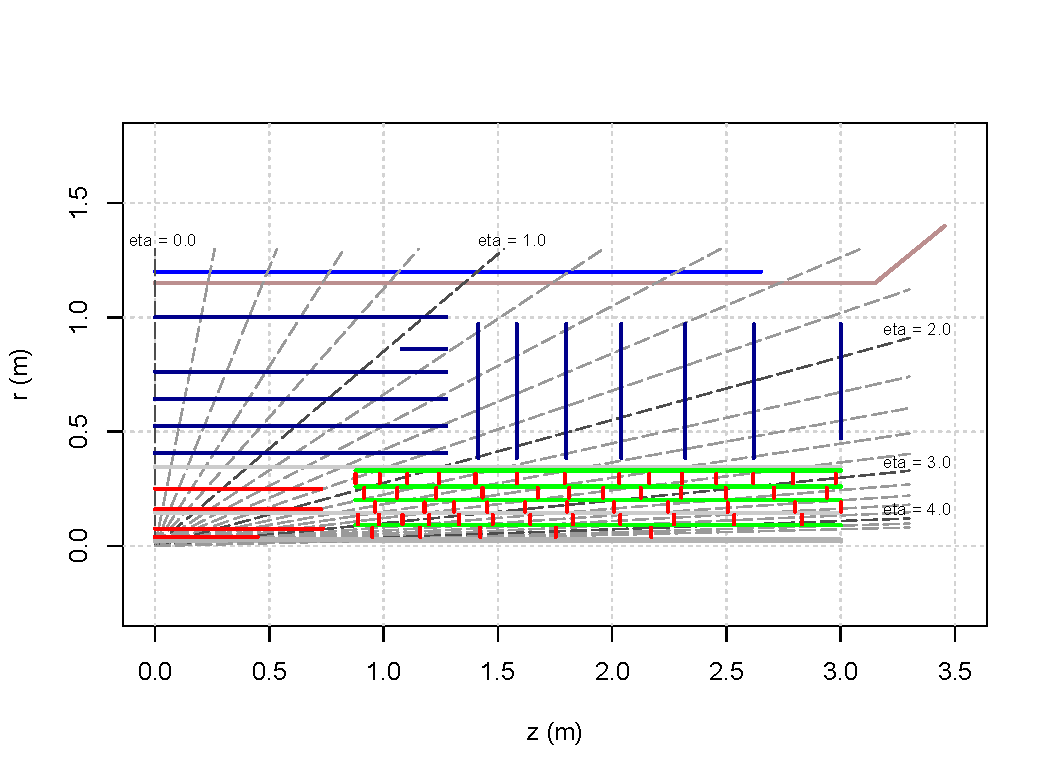
\includegraphics[width=0.90\textwidth]{figures/PLOT-UPGRADE-2014-001/fig_08}
  \caption{Variables.}
  \label{fig:prospects-hllhc-layout}
\end{figure}

\begin{figure}[tp]
  \centering
  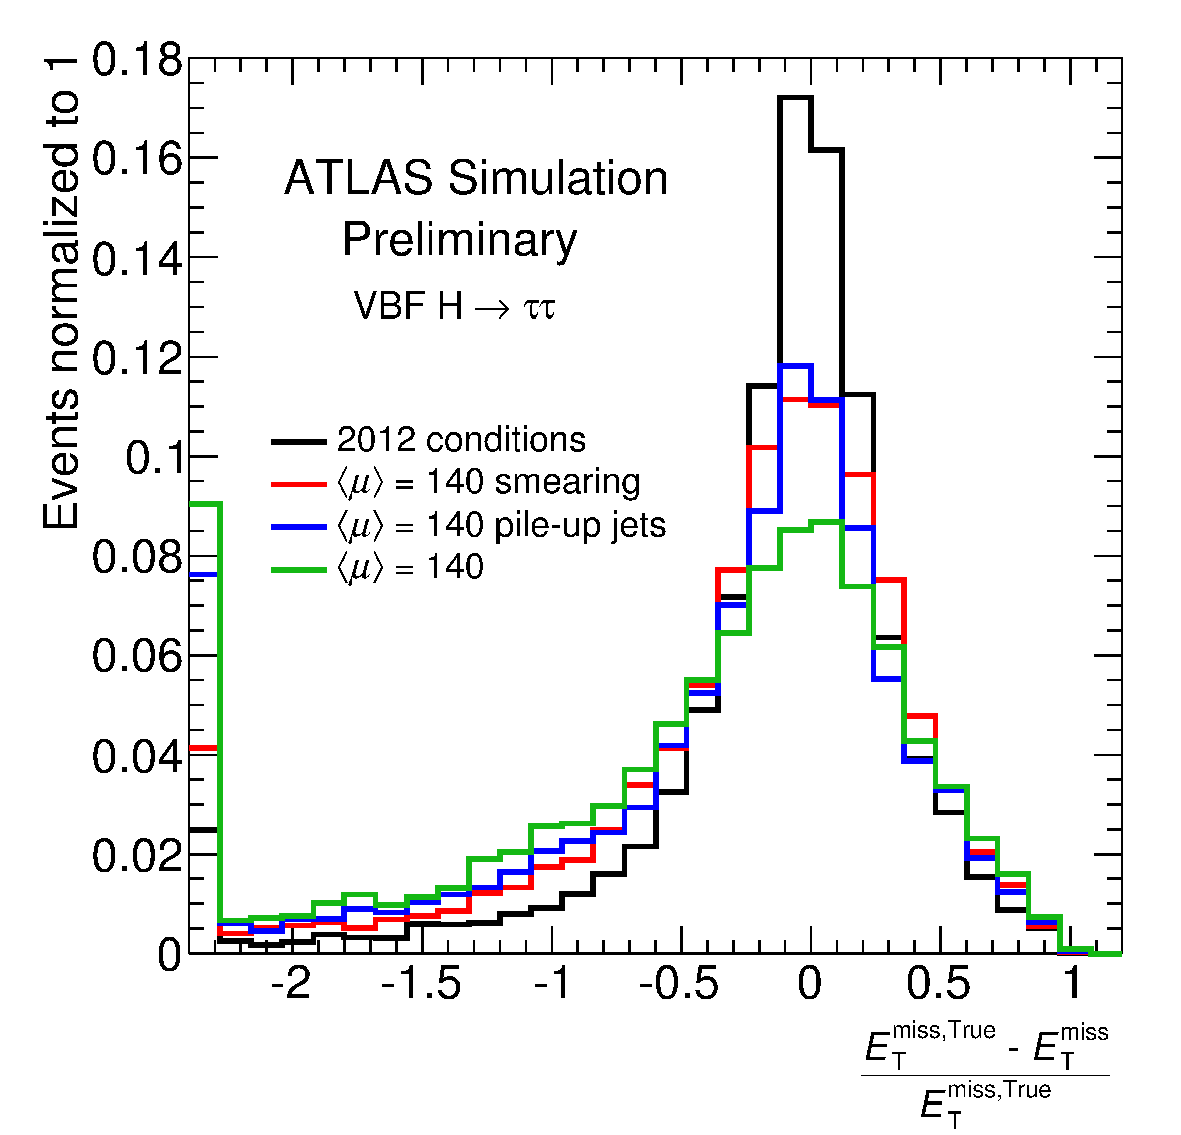
\includegraphics[width=0.48\textwidth]{figures/ATL-PHYS-PUB-2014-018/fig_01a}
  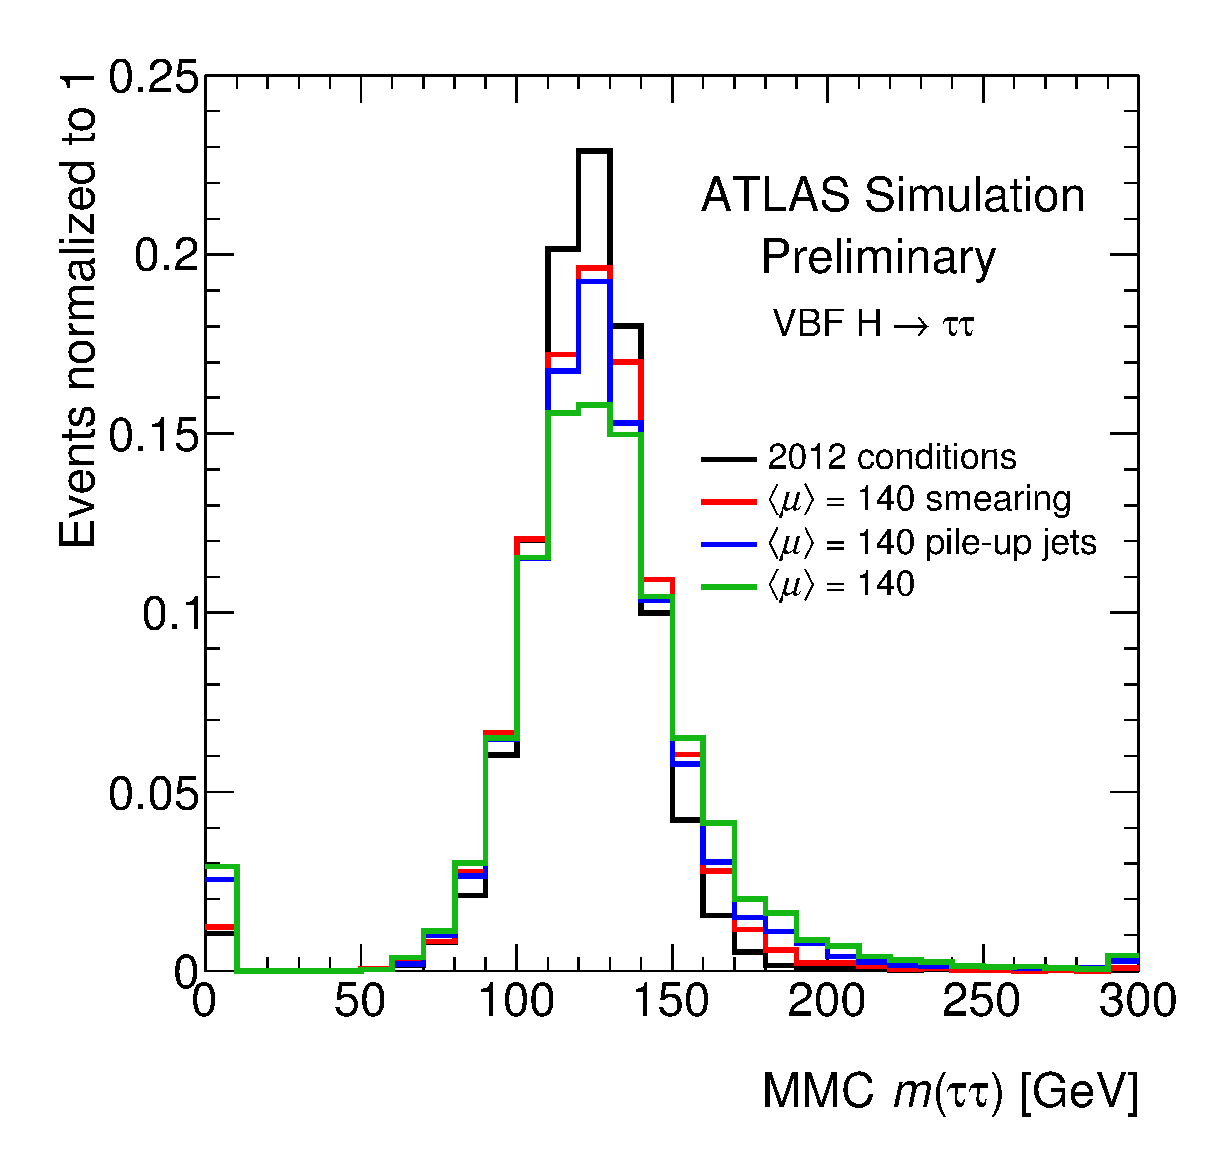
\includegraphics[width=0.48\textwidth]{figures/ATL-PHYS-PUB-2014-018/fig_01b}
  \caption{Variables.}
  \label{fig:prospects-hllhc-degradation}
\end{figure}

\begin{figure}[tp]
  \centering
  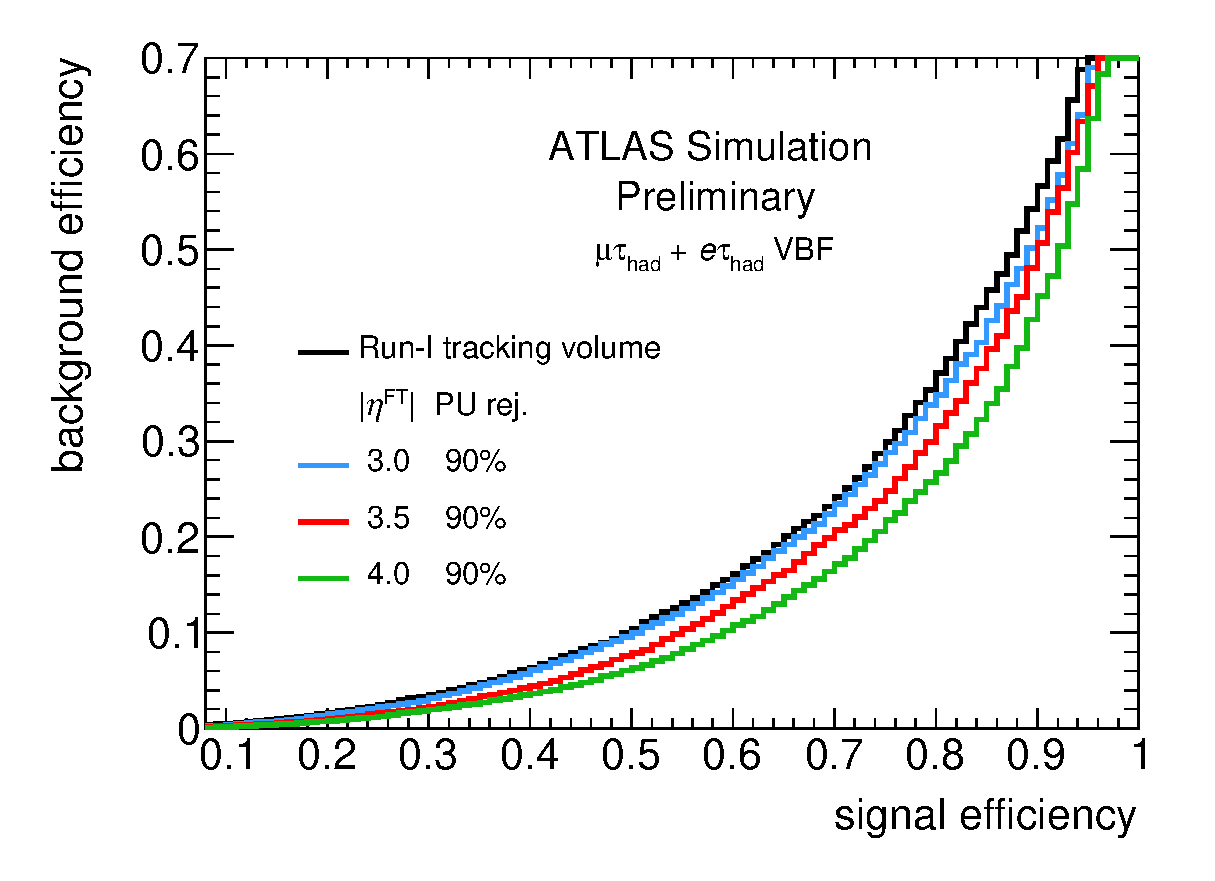
\includegraphics[width=0.48\textwidth]{figures/ATL-PHYS-PUB-2014-018/fig_02a}
  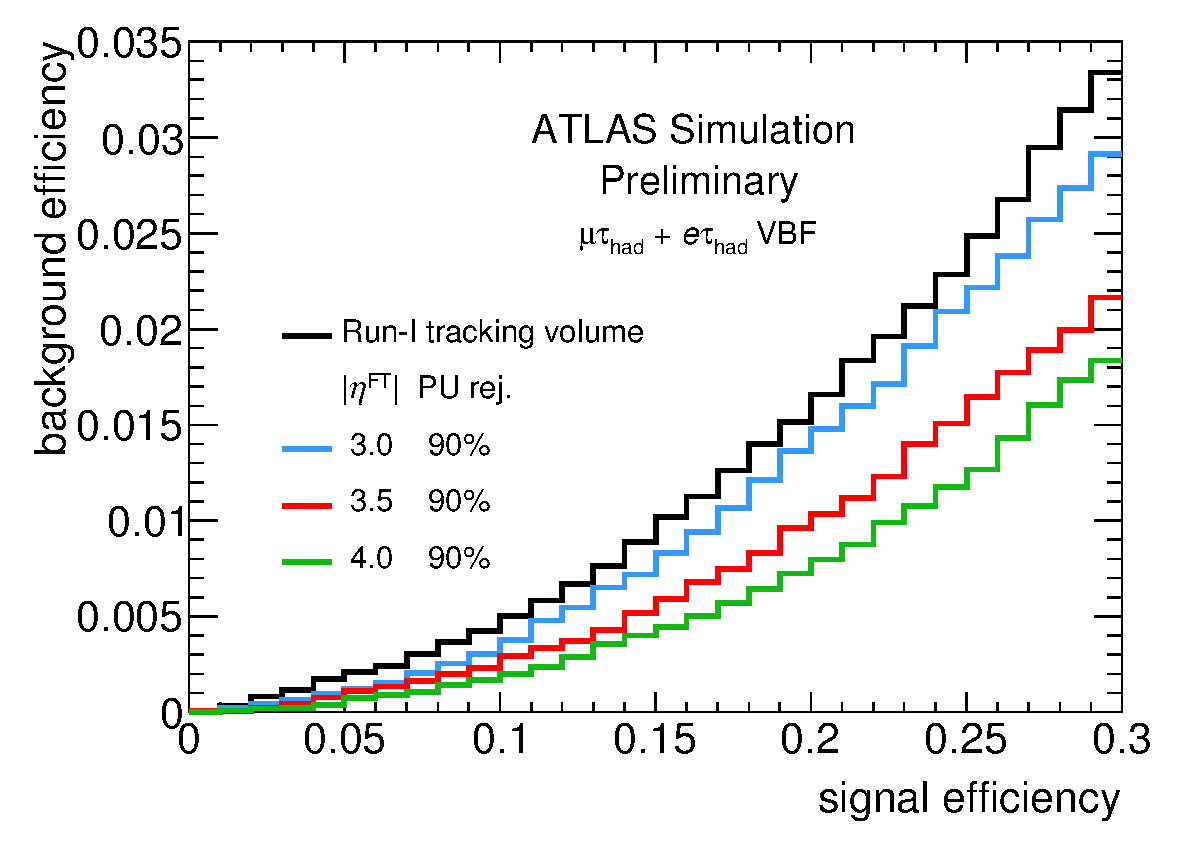
\includegraphics[width=0.48\textwidth]{figures/ATL-PHYS-PUB-2014-018/fig_02b}
  \caption{Variables.}
  \label{fig:prospects-hllhc-rocs}
\end{figure}

\begin{figure}[tp]
  \centering
  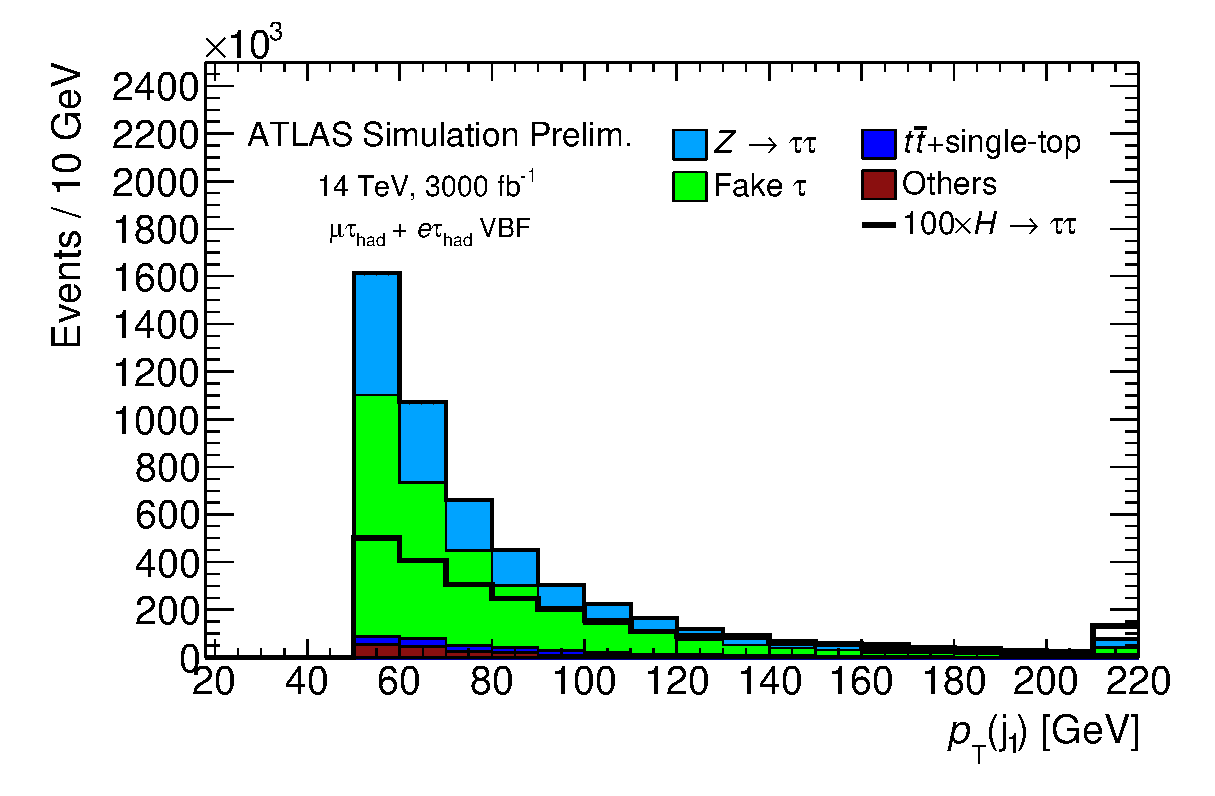
\includegraphics[width=0.48\textwidth]{figures/ATL-PHYS-PUB-2014-018/fig_03a}
  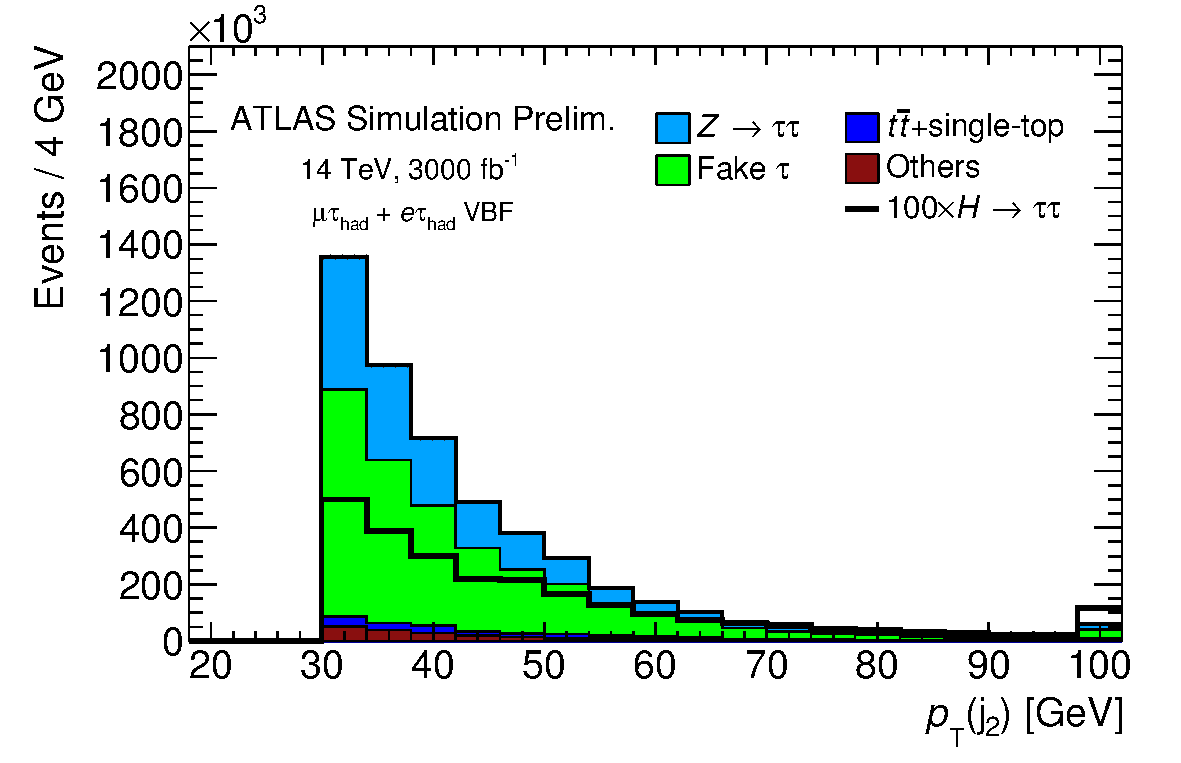
\includegraphics[width=0.48\textwidth]{figures/ATL-PHYS-PUB-2014-018/fig_03b}
  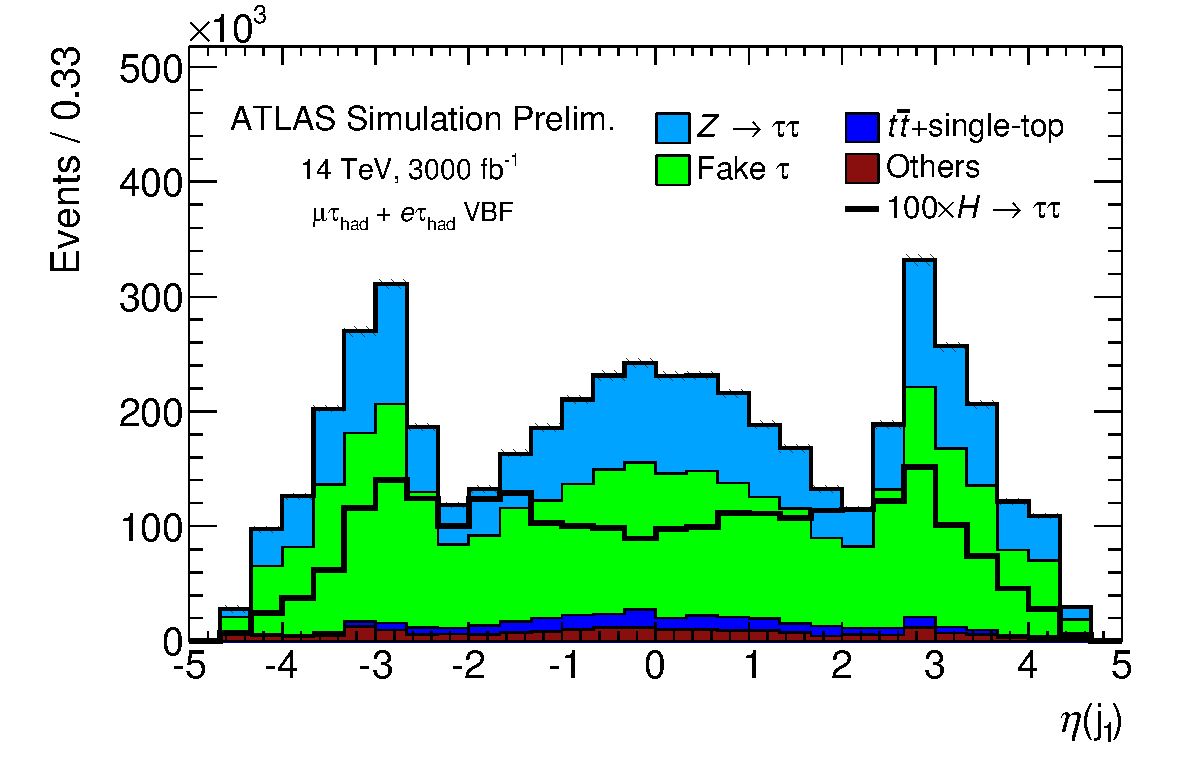
\includegraphics[width=0.48\textwidth]{figures/ATL-PHYS-PUB-2014-018/fig_03c}
  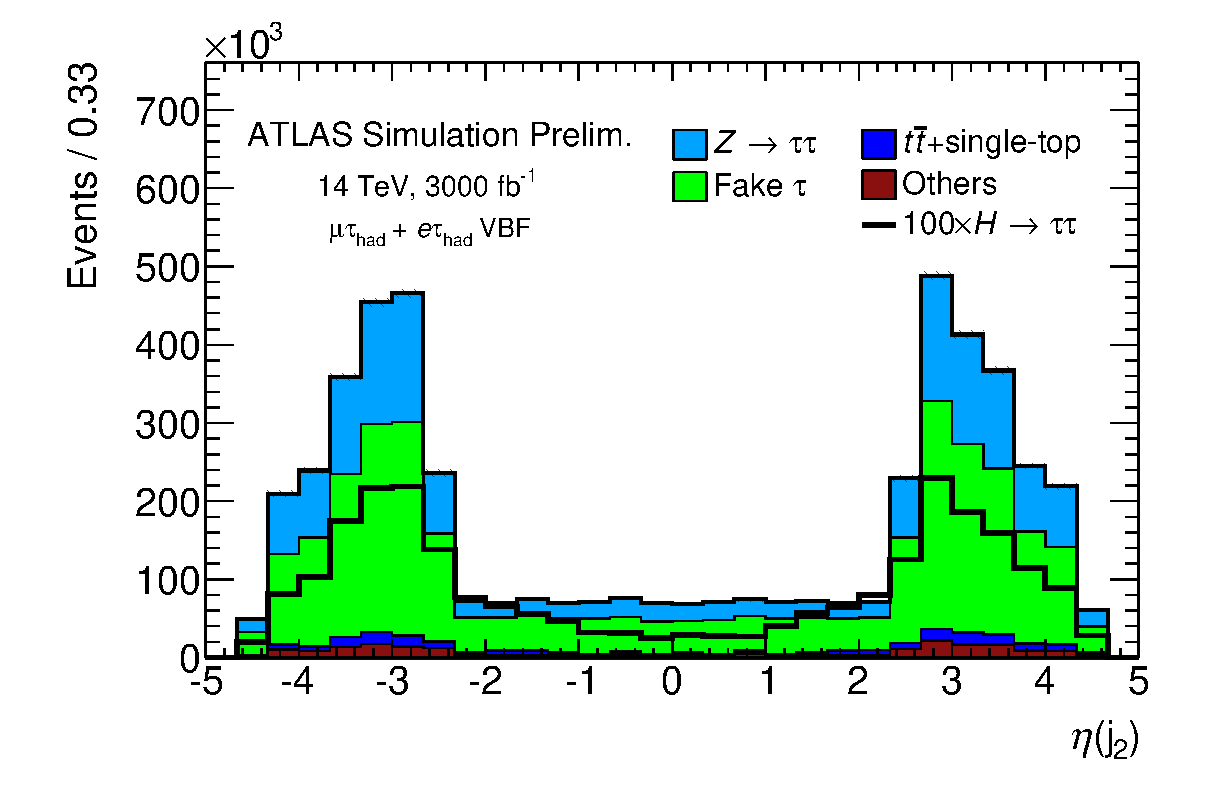
\includegraphics[width=0.48\textwidth]{figures/ATL-PHYS-PUB-2014-018/fig_03d}
  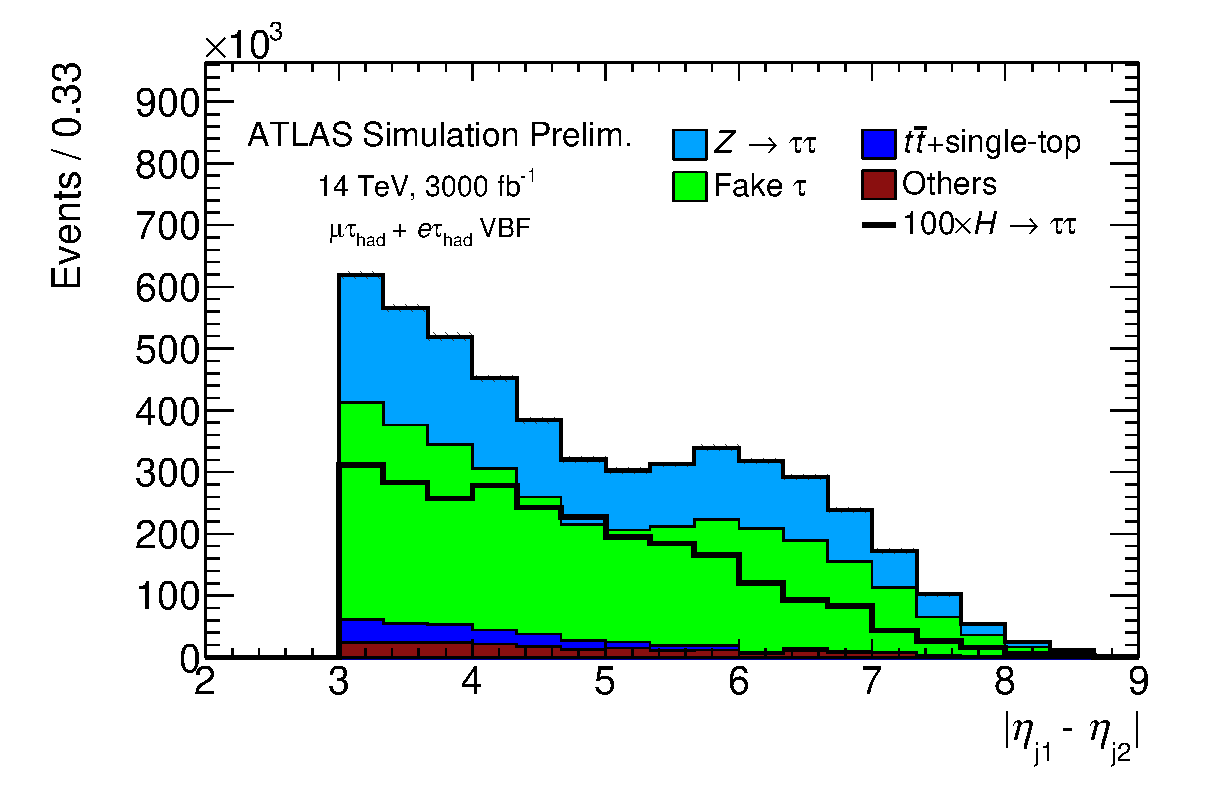
\includegraphics[width=0.48\textwidth]{figures/ATL-PHYS-PUB-2014-018/fig_03e}
  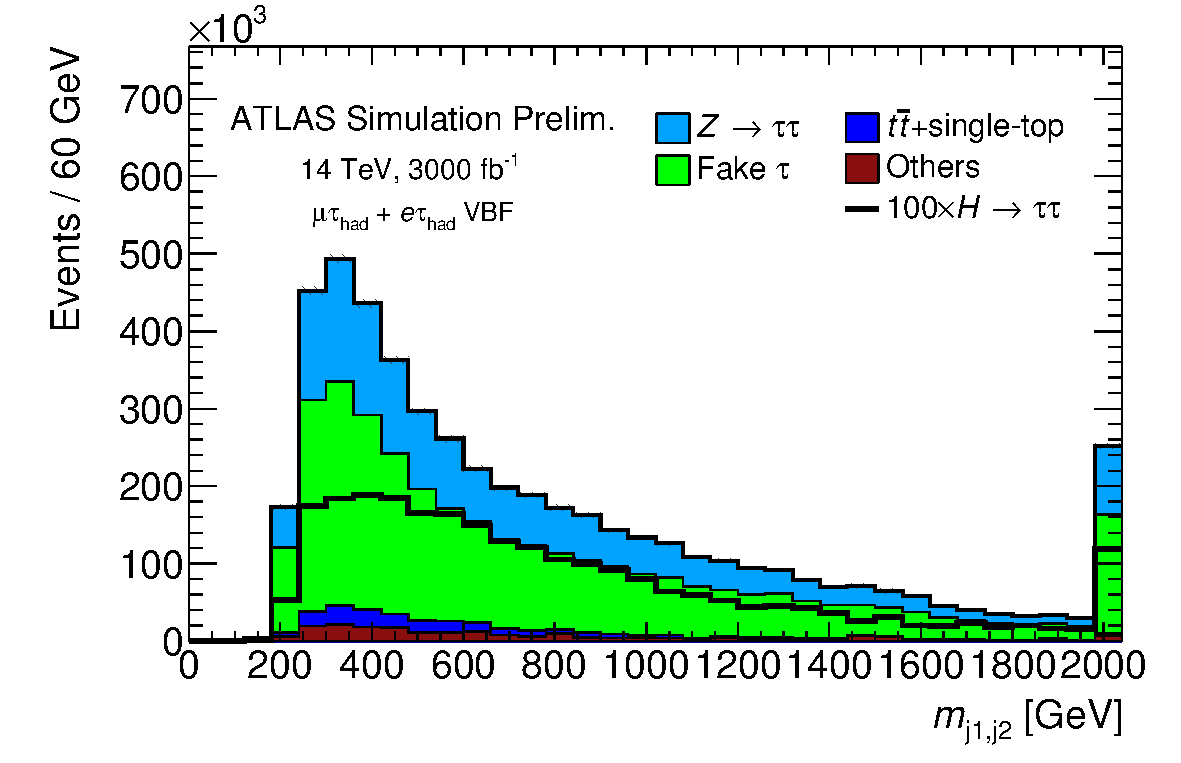
\includegraphics[width=0.48\textwidth]{figures/ATL-PHYS-PUB-2014-018/fig_03f}
  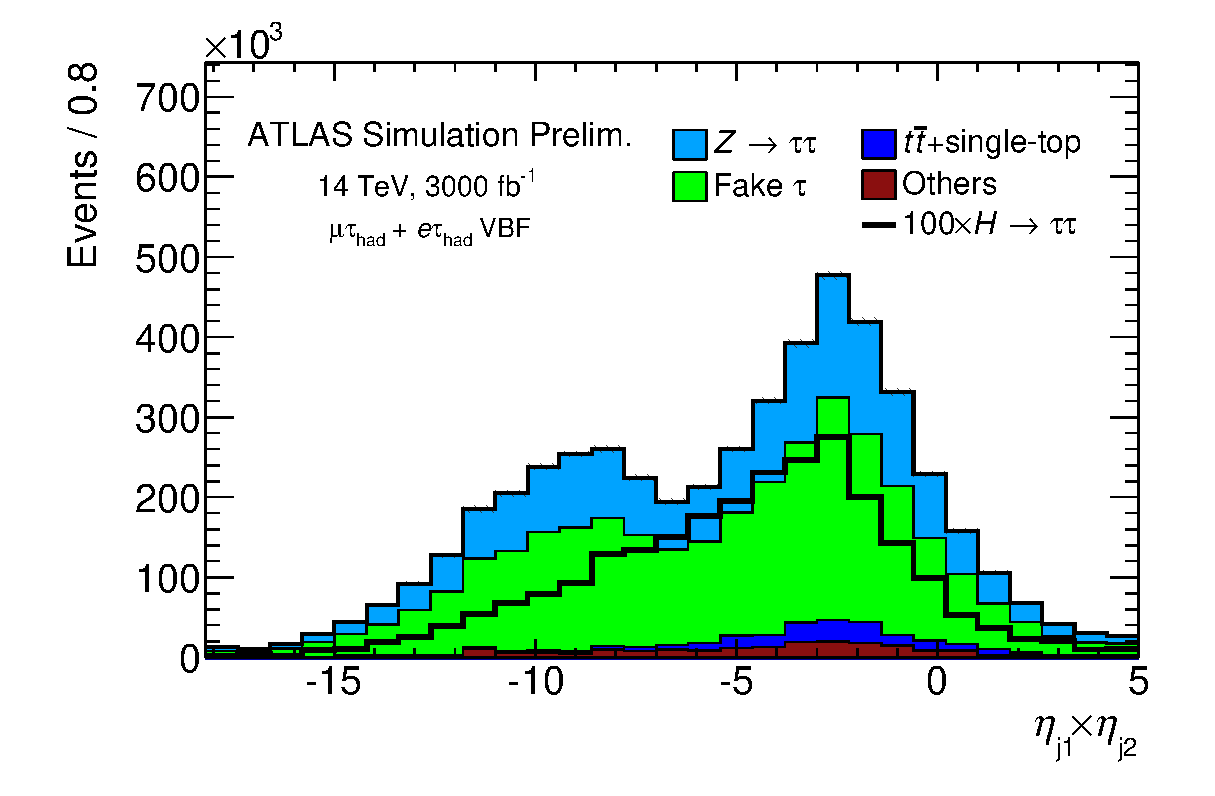
\includegraphics[width=0.48\textwidth]{figures/ATL-PHYS-PUB-2014-018/fig_03g}
  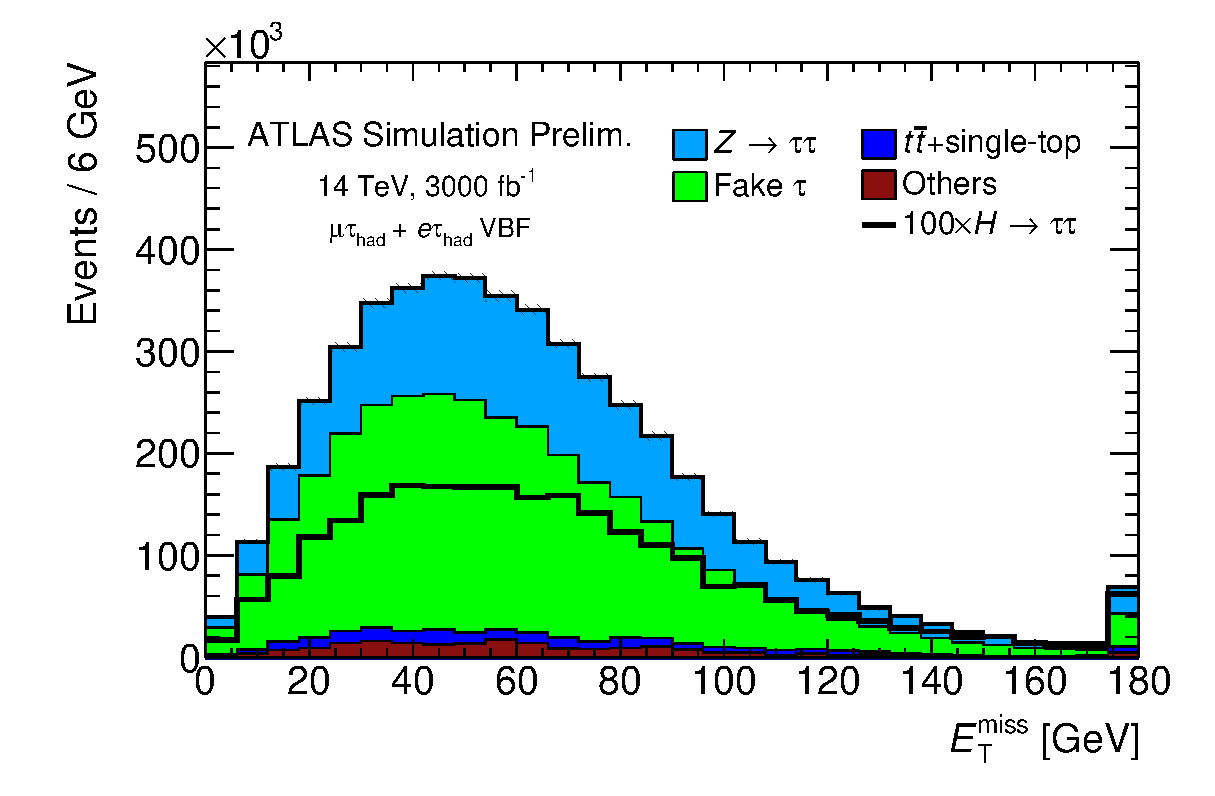
\includegraphics[width=0.48\textwidth]{figures/ATL-PHYS-PUB-2014-018/fig_03h}
  \caption{Variables.}
  \label{fig:prospects-hllhc-jets}
\end{figure}

\begin{figure}[tp]
  \centering
  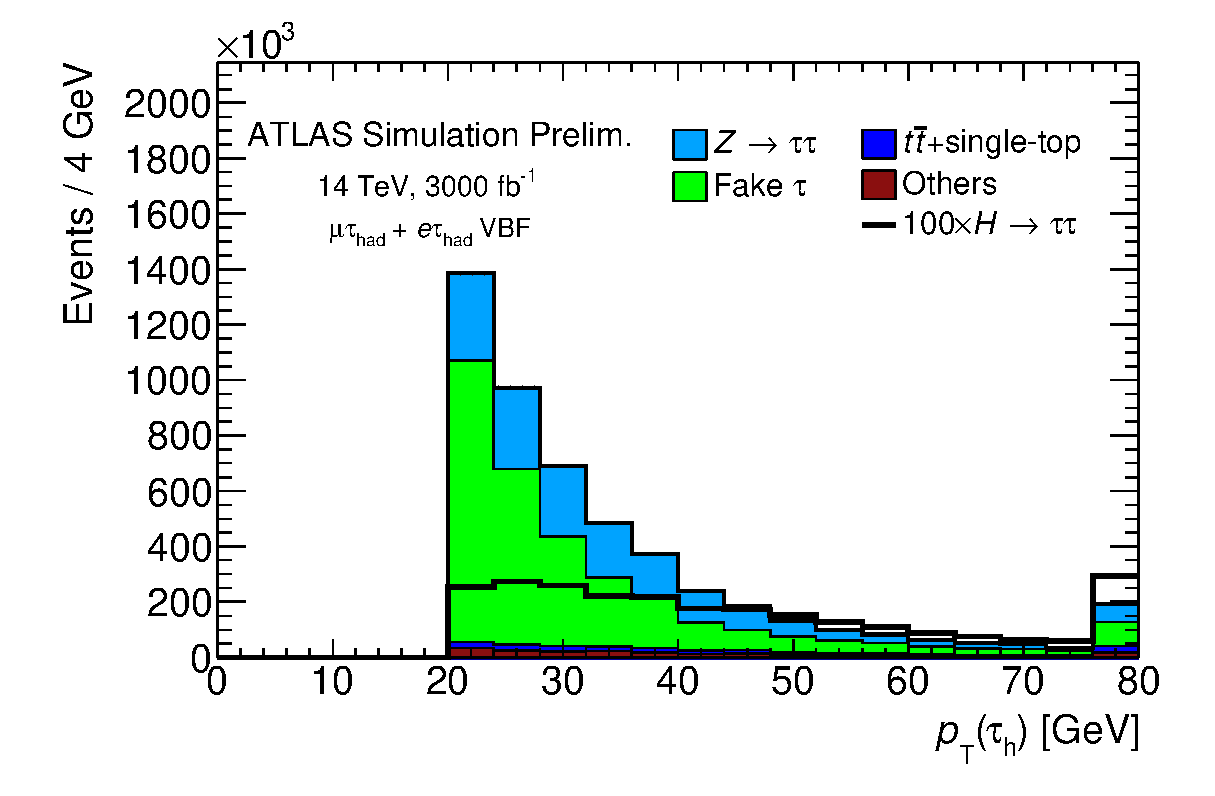
\includegraphics[width=0.48\textwidth]{figures/ATL-PHYS-PUB-2014-018/fig_04a}
  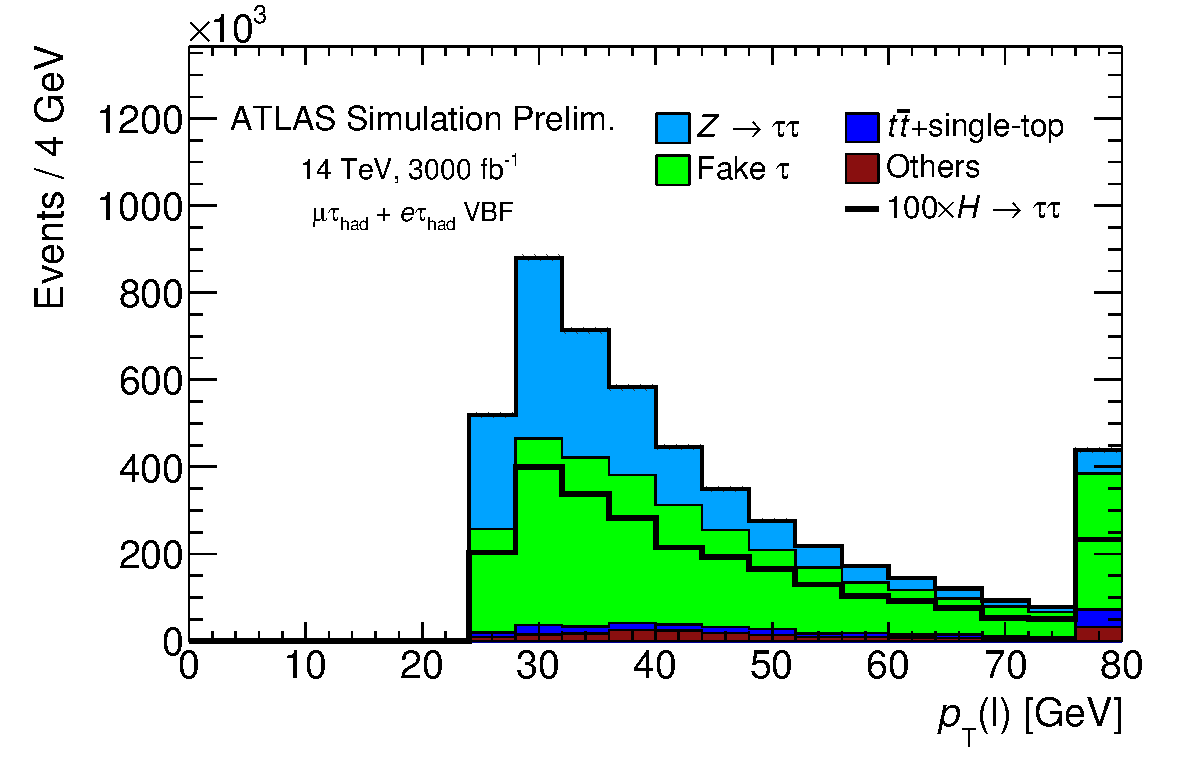
\includegraphics[width=0.48\textwidth]{figures/ATL-PHYS-PUB-2014-018/fig_04b}
  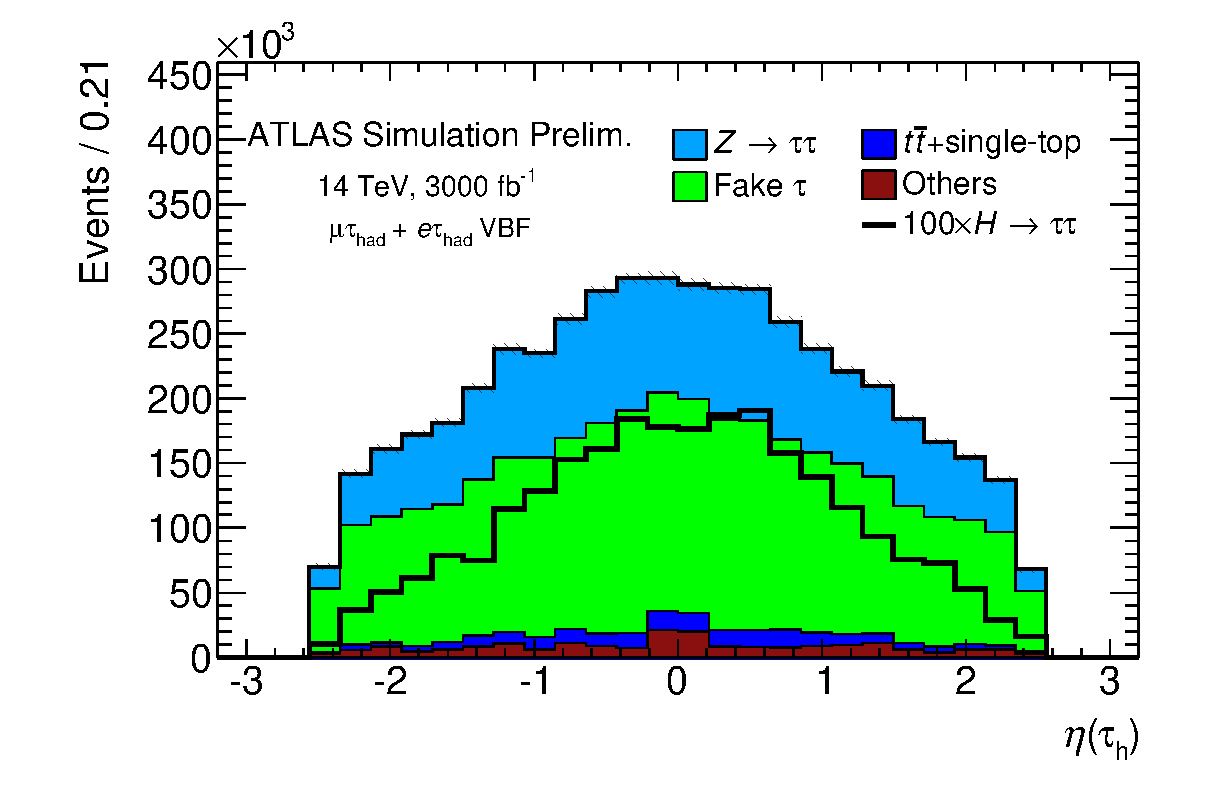
\includegraphics[width=0.48\textwidth]{figures/ATL-PHYS-PUB-2014-018/fig_04c}
  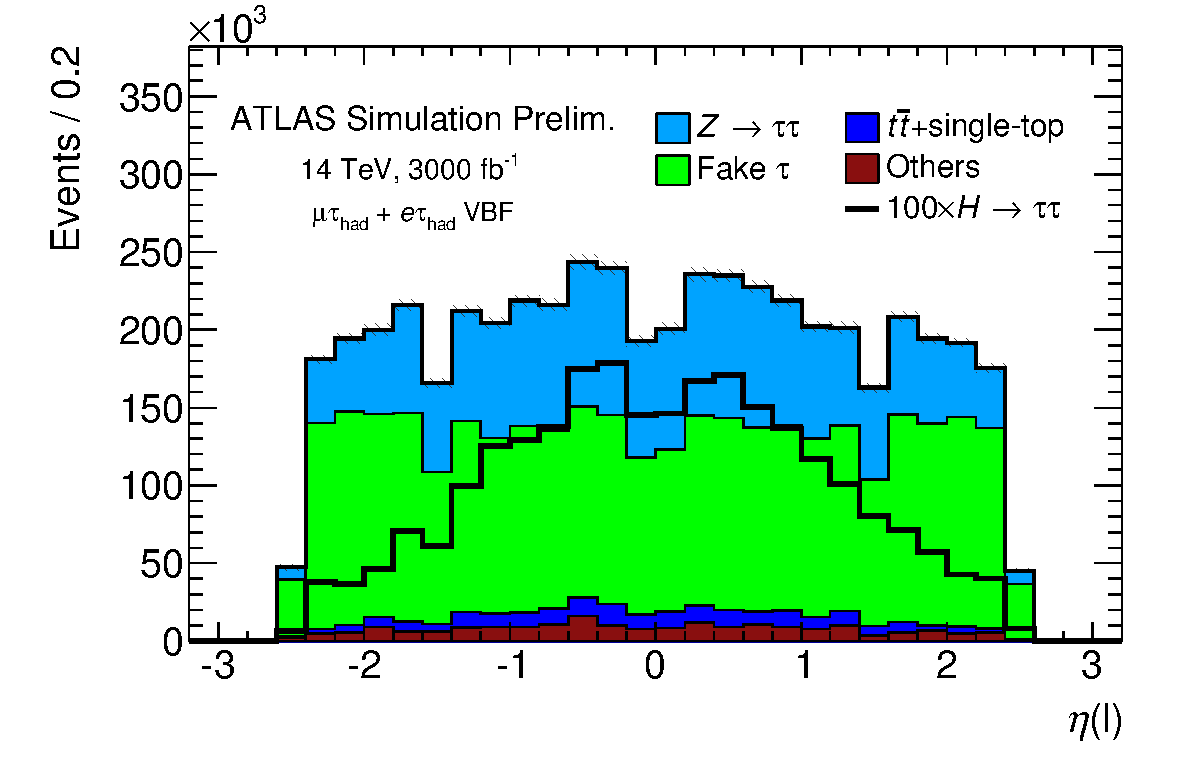
\includegraphics[width=0.48\textwidth]{figures/ATL-PHYS-PUB-2014-018/fig_04d}
  \includegraphics[width=0.48\textwidth]{figures/ATL-PHYS-PUB-2014-018/fig_04e}
  \includegraphics[width=0.48\textwidth]{figures/ATL-PHYS-PUB-2014-018/fig_04f}
  \includegraphics[width=0.48\textwidth]{figures/ATL-PHYS-PUB-2014-018/fig_04g}
  \includegraphics[width=0.48\textwidth]{figures/ATL-PHYS-PUB-2014-018/fig_04h}
  \caption{Variables.}
  \label{fig:prospects-hllhc-taus}
\end{figure}

\begin{figure}[tp]
  \centering
  \includegraphics[width=0.48\textwidth]{figures/ATL-PHYS-PUB-2014-018/fig_06a}
  \includegraphics[width=0.48\textwidth]{figures/ATL-PHYS-PUB-2014-018/fig_06b}
  \caption{Variables.}
  \label{fig:prospects-hllhc-bdts}
\end{figure}


